%
% This is an example LaTeX file which uses the SANDreport class file.
% It shows how a SAND report should be formatted, what sections and
% elements it should contain, and how to use the SANDreport class.
% It uses the LaTeX article class, but not the strict option.
% ItINLreport uses .eps logos and files to show how pdflatex can be used
%
% Get the latest version of the class file and more at
%    http://www.cs.sandia.gov/~rolf/SANDreport
%
% This file and the SANDreport.cls file are based on information
% contained in "Guide to Preparing {SAND} Reports", Sand98-0730, edited
% by Tamara K. Locke, and the newer "Guide to Preparing SAND Reports and
% Other Communication Products", SAND2002-2068P.
% Please send corrections and suggestions for improvements to
% Rolf Riesen, Org. 9223, MS 1110, rolf@cs.sandia.gov
%
\documentclass[pdf,12pt]{INLreport}
% pslatex is really old (1994).  It attempts to merge the times and mathptm packages.
% My opinion is that it produces a really bad looking math font.  So why are we using it?
% If you just want to change the text font, you should just \usepackage{times}.
% \usepackage{pslatex}
\usepackage{times}
\usepackage[FIGBOTCAP,normal,bf,tight]{subfigure}
\usepackage{amsmath}
\usepackage{amssymb}
\usepackage{soul}
\usepackage{bigints}
\usepackage{pifont}
\usepackage{enumerate}
\usepackage{listings}
\usepackage{fullpage}
\usepackage{xcolor}          % Using xcolor for more robust color specification
\usepackage{ifthen}          % For simple checking in newcommand blocks
\usepackage{textcomp}
\usepackage{mathtools}
\usepackage{relsize}
\usepackage{lscape}
\usepackage[toc,page]{appendix}
\newtheorem{mydef}{Definition}
\newcommand{\norm}[1]{\lVert#1\rVert}
%\usepackage[table,xcdraw]{xcolor}
%\usepackage{authblk}         % For making the author list look prettier
%\renewcommand\Authsep{,~\,}

% Custom colors
\definecolor{deepblue}{rgb}{0,0,0.5}
\definecolor{deepred}{rgb}{0.6,0,0}
\definecolor{deepgreen}{rgb}{0,0.5,0}
\definecolor{forestgreen}{RGB}{34,139,34}
\definecolor{orangered}{RGB}{239,134,64}
\definecolor{darkblue}{rgb}{0.0,0.0,0.6}
\definecolor{gray}{rgb}{0.4,0.4,0.4}

\lstset {
  basicstyle=\ttfamily,
  frame=single
}


\setcounter{secnumdepth}{5}
\lstdefinestyle{XML} {
    language=XML,
    extendedchars=true,
    breaklines=true,
    breakatwhitespace=true,
%    emph={name,dim,interactive,overwrite},
    emphstyle=\color{red},
    basicstyle=\ttfamily,
%    columns=fullflexible,
    commentstyle=\color{gray}\upshape,
    morestring=[b]",
    morecomment=[s]{<?}{?>},
    morecomment=[s][\color{forestgreen}]{<!--}{-->},
    keywordstyle=\color{cyan},
    stringstyle=\ttfamily\color{black},
    tagstyle=\color{darkblue}\bf\ttfamily,
    morekeywords={name,type},
%    morekeywords={name,attribute,source,variables,version,type,release,x,z,y,xlabel,ylabel,how,text,param1,param2,color,label},
}
\lstset{language=python,upquote=true}

\usepackage{titlesec}
\newcommand{\sectionbreak}{\clearpage}
\setcounter{secnumdepth}{4}

%\titleformat{\paragraph}
%{\normalfont\normalsize\bfseries}{\theparagraph}{1em}{}
%\titlespacing*{\paragraph}
%{0pt}{3.25ex plus 1ex minus .2ex}{1.5ex plus .2ex}

%%%%%%%% Begin comands definition to input python code into document
\usepackage[utf8]{inputenc}

% Default fixed font does not support bold face
\DeclareFixedFont{\ttb}{T1}{txtt}{bx}{n}{9} % for bold
\DeclareFixedFont{\ttm}{T1}{txtt}{m}{n}{9}  % for normal

\usepackage{listings}

% Python style for highlighting
\newcommand\pythonstyle{\lstset{
language=Python,
basicstyle=\ttm,
otherkeywords={self, none, return},             % Add keywords here
keywordstyle=\ttb\color{deepblue},
emph={MyClass,__init__},          % Custom highlighting
emphstyle=\ttb\color{deepred},    % Custom highlighting style
stringstyle=\color{deepgreen},
frame=tb,                         % Any extra options here
showstringspaces=false            %
}}


% Python environment
\lstnewenvironment{python}[1][]
{
\pythonstyle
\lstset{#1}
}
{}

% Python for external files
\newcommand\pythonexternal[2][]{{
\pythonstyle
\lstinputlisting[#1]{#2}}}

\lstnewenvironment{xml}
{}
{}

% Python for inline
\newcommand\pythoninline[1]{{\pythonstyle\lstinline!#1!}}

% Named Colors for the comments below (Attempted to match git symbol colors)
\definecolor{RScolor}{HTML}{8EB361}  % Sonat (adjusted for clarity)
\definecolor{DPMcolor}{HTML}{E28B8D} % Dan
\definecolor{JCcolor}{HTML}{82A8D9}  % Josh (adjusted for clarity)
\definecolor{AAcolor}{HTML}{8D7F44}  % Andrea
\definecolor{CRcolor}{HTML}{AC39CE}  % Cristian
\definecolor{RKcolor}{HTML}{3ECC8D}  % Bob (adjusted for clarity)
\definecolor{DMcolor}{HTML}{276605}  % Diego (adjusted for clarity)
\definecolor{PTcolor}{HTML}{990000}  % Paul

\def\DRAFT{} % Uncomment this if you want to see the notes people have been adding
% Comment command for developers (Should only be used under active development)
\ifdefined\DRAFT
  \newcommand{\nameLabeler}[3]{\textcolor{#2}{[[#1: #3]]}}
\else
  \newcommand{\nameLabeler}[3]{}
\fi
\newcommand{\alfoa}[1] {\nameLabeler{Andrea}{AAcolor}{#1}}
\newcommand{\cristr}[1] {\nameLabeler{Cristian}{CRcolor}{#1}}
\newcommand{\mandd}[1] {\nameLabeler{Diego}{DMcolor}{#1}}
\newcommand{\maljdan}[1] {\nameLabeler{Dan}{DPMcolor}{#1}}
\newcommand{\cogljj}[1] {\nameLabeler{Josh}{JCcolor}{#1}}
\newcommand{\bobk}[1] {\nameLabeler{Bob}{RKcolor}{#1}}
\newcommand{\senrs}[1] {\nameLabeler{Sonat}{RScolor}{#1}}
\newcommand{\talbpaul}[1] {\nameLabeler{Paul}{PTcolor}{#1}}
% Commands for making the LaTeX a bit more uniform and cleaner
\newcommand{\TODO}[1]    {\textcolor{red}{\textit{(#1)}}}
\newcommand{\xmlAttrRequired}[1] {\textcolor{red}{\textbf{\texttt{#1}}}}
\newcommand{\xmlAttr}[1] {\textcolor{cyan}{\textbf{\texttt{#1}}}}
\newcommand{\xmlNodeRequired}[1] {\textcolor{deepblue}{\textbf{\texttt{<#1>}}}}
\newcommand{\xmlNode}[1] {\textcolor{darkblue}{\textbf{\texttt{<#1>}}}}
\newcommand{\xmlString}[1] {\textcolor{black}{\textbf{\texttt{'#1'}}}}
\newcommand{\xmlDesc}[1] {\textbf{\textit{#1}}} % Maybe a misnomer, but I am
                                                % using this to detail the data
                                                % type and necessity of an XML
                                                % node or attribute,
                                                % xmlDesc = XML description
\newcommand{\default}[1]{~\\*\textit{Default: #1}}
\newcommand{\nb} {\textcolor{deepgreen}{\textbf{~Note:}}~}


%%%%%%%% End comands definition to input python code into document

%\usepackage[dvips,light,first,bottomafter]{draftcopy}
%\draftcopyName{Sample, contains no OUO}{70}
%\draftcopyName{Draft}{300}

% The bm package provides \bm for bold math fonts.  Apparently
% \boldsymbol, which I used to always use, is now considered
% obsolete.  Also, \boldsymbol doesn't even seem to work with
% the fonts used in this particular document...
\usepackage{bm}


% Define tensors to be in bold math font.
\newcommand{\tensor}[1]{{\bm{#1}}}

% Override the formatting used by \vec.  Instead of a little arrow
% over the letter, this creates a bold character.
\renewcommand{\vec}{\bm}

% Define unit vector notation.  If you don't override the
% behavior of \vec, you probably want to use the second one.
\newcommand{\unit}[1]{\hat{\bm{#1}}}
% \newcommand{\unit}[1]{\hat{#1}}

% Use this to refer to a single component of a unit vector.
\newcommand{\scalarunit}[1]{\hat{#1}}

% \toprule, \midrule, \bottomrule for tables
\usepackage{booktabs}

% \llbracket, \rrbracket
\usepackage{stmaryrd}

\usepackage{hyperref}
\hypersetup{
    colorlinks,
    citecolor=black,
    filecolor=black,
    linkcolor=black,
    urlcolor=black
}

% Compress lists of citations like [33,34,35,36,37] to [33-37]
\usepackage{cite}

% If you want to relax some of the SAND98-0730 requirements, use the "relax"
% option. It adds spaces and boldface in the table of contents, and does not
% force the page layout sizes.
% e.g. \documentclass[relax,12pt]{SANDreport}
%
% You can also use the "strict" option, which applies even more of the
% SAND98-0730 guidelines. It gets rid of section numbers which are often
% useful; e.g. \documentclass[strict]{SANDreport}

% The INLreport class uses \flushbottom formatting by default (since
% it's intended to be two-sided document).  \flushbottom causes
% additional space to be inserted both before and after paragraphs so
% that no matter how much text is actually available, it fills up the
% page from top to bottom.  My feeling is that \raggedbottom looks much
% better, primarily because most people will view the report
% electronically and not in a two-sided printed format where some argue
% \raggedbottom looks worse.  If we really want to have the original
% behavior, we can comment out this line...
\raggedbottom
\setcounter{secnumdepth}{5} % show 5 levels of subsection
\setcounter{tocdepth}{5} % include 5 levels of subsection in table of contents

% ---------------------------------------------------------------------------- %
%
% Set the title, author, and date
%
\title{RAVEN Theory Manual}
%\author{%
%\begin{tabular}{c} Author 1 \\ University1 \\ Mail1 \\ \\
%Author 3 \\ University3 \\ Mail3 \end{tabular} \and
%\begin{tabular}{c} Author 2 \\ University2 \\ Mail2 \\ \\
%Author 4 \\ University4 \\ Mail4\\
%\end{tabular} }


\author{
\\Andrea Alfonsi
\\Cristian Rabiti
\\Diego Mandelli
\\Joshua Cogliati
\\Congjian Wang
\\Paul W. Talbot
\\Daniel P. Maljovec
\\Curtis Smith
}
% \\James B. Tompkins}   Just people who actually ``developed'' a significant capability in the code should be placed here. Andrea
%\author{\textbf{\textit{Main Developers:}}  \\Andrea Alfonsi}
%\affil{Idaho National Laboratory, Idaho Falls, ID 83402}
%\\\{cristian.rabiti, andrea.alfonsi, joshua.cogliati, diego.mandelli, robert.kinoshita, ramazan.sen\}@inl.gov}

% There is a "Printed" date on the title page of a SAND report, so
% the generic \date should [WorkingDir:]generally be empty.
\date{}


% ---------------------------------------------------------------------------- %
% Set some things we need for SAND reports. These are mandatory
%
\SANDnum{INL/EXT-16-38178}
\SANDprintDate{March 2016}
\SANDauthor{Andrea Alfonsi, Cristian Rabiti, Diego Mandelli, Joshua Cogliati, Congjian Wang, Paul W. Talbot, Daniel P. Maljovec, Curtis Smith}
\SANDreleaseType{Revision 0 Draft}


% ---------------------------------------------------------------------------- %
% Include the markings required for your SAND report. The default is "Unlimited
% Release". You may have to edit the file included here, or create your own
% (see the examples provided).
%
% \include{MarkOUO} % Not needed for unlimted release reports

\def\component#1{\texttt{#1}}

% ---------------------------------------------------------------------------- %
\newcommand{\systemtau}{\tensor{\tau}_{\!\text{SUPG}}}

% Added by Sonat
\usepackage{placeins}
\usepackage{array}

\newcolumntype{L}[1]{>{\raggedright\let\newline\\\arraybackslash\hspace{0pt}}m{#1}}
\newcolumntype{C}[1]{>{\centering\let\newline\\\arraybackslash\hspace{0pt}}m{#1}}
\newcolumntype{R}[1]{>{\raggedleft\let\newline\\\arraybackslash\hspace{0pt}}m{#1}}

% end added by Sonat
% ---------------------------------------------------------------------------- %
%
% Start the document
%

\begin{document}
    \maketitle

    % ------------------------------------------------------------------------ %
    % An Abstract is required for SAND reports
    %
%    \begin{abstract}
%    \input abstract
%    \end{abstract}


    % ------------------------------------------------------------------------ %
    % An Acknowledgement section is optional but important, if someone made
    % contributions or helped beyond the normal part of a work assignment.
    % Use \section* since we don't want it in the table of context
    %
%    \clearpage
%    \section*{Acknowledgment}



%	The format of this report is based on information found
%	in~\cite{Sand98-0730}.


    % ------------------------------------------------------------------------ %
    % The table of contents and list of figures and tables
    % Comment out \listoffigures and \listoftables if there are no
    % figures or tables. Make sure this starts on an odd numbered page
    %
    \cleardoublepage		% TOC needs to start on an odd page
    \tableofcontents
    %\listoffigures
    %\listoftables


    % ---------------------------------------------------------------------- %
    % An optional preface or Foreword
%    \clearpage
%    \section*{Preface}
%    \addcontentsline{toc}{section}{Preface}
%	Although muggles usually have only limited experience with
%	magic, and many even dispute its existence, it is worthwhile
%	to be open minded and explore the possibilities.


    % ---------------------------------------------------------------------- %
    % An optional executive summary
    %\clearpage
    %\section*{Summary}
    %\addcontentsline{toc}{section}{Summary}
    %RAVEN is a bird

%	Once a certain level of mistrust and skepticism has
%	been overcome, magic finds many uses in todays science



%	and engineering. In this report we explain some of the
%	fundamental spells and instruments of magic and wizardry. We
%	then conclude with a few examples on how they can be used
%	in daily activities at national Laboratories.


    % ---------------------------------------------------------------------- %
    % An optional glossary. We don't want it to be numbered
%    \clearpage
%    \section*{Nomenclature}
%    \addcontentsline{toc}{section}{Nomenclature}
%    \begin{description}
%          \item[alohomoral]
%           spell to open locked doors and containers
%          \item[leviosa]
%           spell to levitate objects
%    \item[remembrall]
%           device to alert you that you have forgotten something
%    \item[wand]
%           device to execute spells
%    \end{description}


    % ---------------------------------------------------------------------- %
    % This is where the body of the report begins; usually with an Introduction
    %
    \SANDmain		% Start the main part of the report

\label{sec:introduction}
RAVEN (\textbf{R}eactor \textbf{A}nalysis and \textbf{V}irtual control \textbf{EN}viroment)~\cite{ravenFY12,mandelliANS2012} is a software tool that acts as the control logic driver for the newly developed Thermal-Hydraulic code RELAP-7  (\textbf{R}eactor \textbf{E}xcursion and \textbf{L}eak \textbf{A}nalysis \textbf{P}rogram). 
RAVEN has been designed in a high modular and pluggable way in order to enable easy integration of different programming languages (i.e., C++, Python) and coupling with other applications including the ones based on the MOOSE framework, developed by INL as well.
\\The goal of this report is to highlight the newly developed  Dynamic Event Tree (DET) module embedded in the code and its utilization in conjunction with RELAP-7. 

As for all \textbf{P}robabilistic \textbf{R}isk \textbf{A}ssessment (PRA) software the capability to fully control the plant evolution during the simulation represents a highly desirable feature as it is for the analysis of the propagation of the uncertainty. . For these reasons, a strict interaction between RELAP-7 and RAVEN is a key of the long-term success of the overall project. In system safety analysis codes, a similar need is expressed by the implementation of the control logic of the plant. As a consequence the optimization of resources imposes the integration of this task under a common project that is naturally RAVEN.The final outcome is a very general and flexible implementation of the plant control logic that will easily allow the integration of proprietary information without any change in the RELAP-7 code. This is also regarded as a facilitating factor for the quick deployment of RELAP-7.

In order to summarize what RAVEN is, it can be said that it is a multi-purpose PRA software framework that allows dispatching different functionalities. 
It is designed to derive and actuate the control logic required to simulate the plant control system and operator actions (guided procedures) and to perform both Monte-Carlo sampling  and Event Tree based analysis of the probabilistic behavior of the NPP. 
In order to facilitate the input/output handling, a \textbf{G}raphical \textbf{U}ser \textbf{I}nterface (GUI) and a post-processing data mining module (under development) are available.

This report provides an overview of the DET structure, highlighting the mathematical framework from which its structure is derived and its software implementation. In addition a \textbf{S}tation \textbf{B}lack \textbf{O}ut (SBO) DET based analysis of a simplified \textbf{P}ressurized \textbf{W}ater \textbf{R}eactor (PWR) model will be shown.
\vspace{-5mm}

%\subsection{subsection}
%text

%figure template

%\subsubsection{subsubsection}
%more text
%\paragraph{paragraph} 
%lot of text
%\subparagraph{subparagraph} 
%if you arrive at this point you have issues

\section{Introduction}


\subsection{System Purpose}

The RAVEN code is a generic software framework to perform parametric
and probabilistic analysis based on the response of complex system
codes. RAVEN is capable of investigating the system response as well
as the input space using Monte Carlo, Grid, or Latin Hyper Cube
sampling schemes, but its strength is focused toward system feature
discovery, such as limit surfaces, separating regions of the input
space leading to system failure, using dynamic supervised learning
techniques.

The development of RAVEN started in 2012 to satisfy the need to
provide a modern risk evaluation framework. RAVEN's principal
assignment is to provide the necessary software and algorithms in
order to employ the concept developed by the Risk Informed Safety
Margin Characterization (RISMC) program. RISMC is one of the pathways
defined within the Light Water Reactor Sustainability (LWRS)
program. In the RISMC approach, the goal is not just specifically
identifying the frequency of an event potentially leading to a system
failure, but the closeness (or not) to key safety-related events. This
approach may be used in identifying and increasing the safety margins
related to those events. A safety margin is a numerical value
quantifying the probability that a safety metric (e.g. as peak
pressure in a pipe) is exceeded under certain conditions. The initial
development of RAVEN has been focused on providing dynamic risk
assessment capability to the MOOSE application RELAP-7, currently
under development at the INL and, the likely future replacement of the
RELAP5-3D code. Most of the capabilities implemented using RELAP-7 are
easily deployable for other system codes.

\subsection{System Scope}

The produced product is the RAVEN software.  It is a computer
code designed for probabilistic analysis.  RAVEN is a statistical
analysis tool that is used to estimate risk by computing real numbers
to determine what can go wrong, how likely is it, and what are its
consequences.  RAVEN takes in input (such as input files for
subprograms, or CSV files of data) and then can run subprograms with
perturbed input to calculate the result of physical simulations with
varying input parameters.  Then RAVEN takes the output of those
program or the data provided and performs statistical analysis on the
data.

\subsection{Other Design Documentation}

In addition to this document, with every merge request developer
documentation is automatically extracted from the source code using
Doxygen and is available to developers at
\url{https://hpcsc.inl.gov/ssl/RAVEN/docs/classes.html}

The software is under configuration management process identified in
`` Configuration Management Plan for Modeling and Simulation
Software'' PLN-4004 Revision 3.

\subsection{Definitions and Acronyms}

\begin{description}
\item[API] Application Programming Interfaces
\item[CDF] Cumulative Distribution Function
\item[DET] Dynamic Event Tree
\item[LWRS] Light Water Reactor Sustainability
\item[MC] Monte Carlo
\item[MOOSE] Multiphysics Object-Oriented Simulation Environment
\item[PDF] Probability Distribution Function
\item[RAVEN] Risk Analysis Virtual ENvironment
\item[RELAP-7] Reactor Excursion and Leak Analysis Program v.7
\item[RISMC] Risk Informed Safety Margin Characterization
\item[ROM] Reduced Order Model
\end{description}


\subsection{Software infrastructure}
\subsubsection{Outlines}
RAVEN has been developed in a highly modular and pluggable way in order to enable easy integration of different programming languages (i.e., C++, Python) and, as already mentioned, coupling with any system code.

\subsubsection{Probabilistic and Parametric framework}
The probabilistic and parametric framework represents the core of the RAVEN analysis capabilities. The main idea behind the design of the system is the creation of a multipurpose framework characterized by high flexibility with respect to the possible performable analysis. The framework must be capable of constructing the analysis/calculation flow at run-time, interpreting the user-defined instructions and assembling the different analysis tasks following a user specified scheme.
In order to achieve such flexibility, combined with reasonably fast development, a programming language naturally suitable for this kind of approach was needed: $Python$.


\begin{figure}[ht]
  \centering
  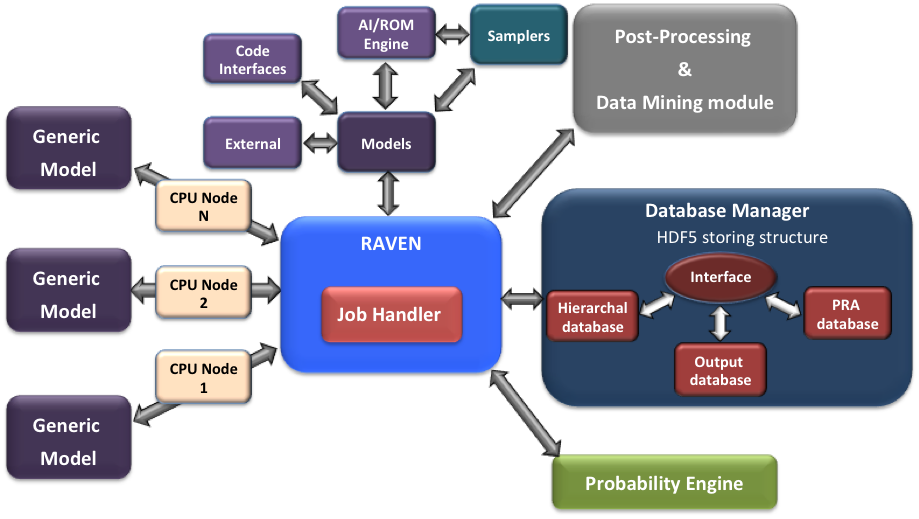
\includegraphics[width=1.0\textwidth]  {pics/RavenFramework.png}
  \caption{RAVEN framework layout}
  \label{fig:RAVENframeworkLayout}
\end{figure}

Hence, RAVEN is coded in $Python$ and is characterized by an object-oriented design. The core of the analysis performable through RAVEN is represented by a set of basic components (objects) the user can combine, in order to create a custom analysis flow. A list of these components and a summary of their most important functionalities are reported as follows:
\begin{itemize}
\item	Distribution: In order to explore the input/output space, RAVEN requires the capability to perturb the input space (initial conditions and/or model coefficients of a system code). The input space is generally characterized by probability distribution functions (PDFs), which might need to be considered when a perturbation is applied. In this respect, a large library of PDFs is available.
\item Sampler: A proper approach to sample the input space is fundamental for the optimization of the computational time. In RAVEN, a ``sampler'' employs a unique perturbation strategy that is applied to the input space of a system. The input space is defined through the connection of uncertain variables and their relative probability distributions.
\item Model: A model is the representation of a physical system (e.g. Nuclear Power Plant); it is therefore capable of predicting the evolution of a system given a coordinate set in the input space. In addition it can represent an
action on a data in order to extract key features (e.g. Data mining).
\item Reduced Order Model (ROM): The evaluation of the system response, as a function of the coordinates in the input space, is very computationally expensive, especially when brute-force approaches (e.g. Monte Carlo methods) are chosen as the sampling strategy. ROMs are used to lower this cost, reducing the number of needed points and prioritizing the area of the input space that needs to be explored. They can be considered as an artificial representation of the link between the input and output spaces for a particular system.
\end{itemize}
The list above is not comprehensive of all the RAVEN framework components (visualization and storage infrastructure).
\\ Figure~\ref{fig:RAVENframeworkLayout} shows a schematic representation of the whole framework, highlighting the communication pipes among the different modules and engines. As can be seen, in the figure all the components reported above are schematically shown. In addition the data management, mining and processing modules are shown.

\subsubsection{Distribution}
As already mentioned, the perturbation of the input space, through the initial conditions (parameters) affected by uncertainties, needs to be performed by the proper distribution functions. RAVEN provides, through an interface to the BOOST library, the following variate (truncated and not) distributions: Bernoulli, Binomial, Exponential, Logistic, Lognormal, Normal, Poisson, Triangular, Uniform, Weibull, Gamma, and Beta.
\\The usage of uni-variate distributions for sampling initial conditions is based on the assumption that the uncertain parameters are not correlated with each other. Quite often uncertain parameters are subject to correlations and thus the uni-variate approach is not applicable. This happens when a generic outcome is dependent on different phenomena simultaneously (i.e. the outcome dependency description can not be collapsed to a function of a single variable). RAVEN currently supports both N-dimensional (N-D) PDFs. The user can provide the distribution values on either Cartesian or sparse grid, which determines the interpolation algorithm used in the evaluation of the imported CDF/PDF:
\begin{enumerate}
\item N-Dimensional Spline, for Cartesian grids
\item Inverse weight, for sparse grids
\end{enumerate}
Internally, RAVEN provides the needed N-D differentiation and integration algorithms to compute the PDF from the CDF and vice-versa.
\\As already mentioned, the sampling methods use the distributions in order to perform probability-weighted perturbations. For example, in the Monte Carlo approach, a random number $\in [0,1]$ is generated (probability threshold) and the CDF, corresponding to that probability, is inverted in order to retrieve the parameter value usable in the simulation. The existence of the inverse for variate distributions is guaranteed by the monotonicity of the CDF. For N-D distributions this condition is not sufficient since the $CDF(X)\longrightarrow [0,1],X \in  R^{N} $ and therefore it could not be a bijective function. From an application point of view, this means the inverse of a N-D CDF is not unique.
\\As an example, the Figure~\ref{fig:NDDistributionExample} shows a multivariate normal distribution for a pipe failure as function of the pressure and temperature. The plane identifies an isoprobability surface (in this case, a line) that represents a probability threshold of 50 \% in this example.  Hence, the inverse of this CDF is an infinite number of points.
 \\As easily inferable, the standard sampling approach cannot directly be employed. When multivariate distributions are used, RAVEN implements a surface search algorithm for identifying the iso-probability surface location. Once the location of the surface has been found, RAVEN chooses, randomly, one point on it.

\begin{figure}
  \centering
  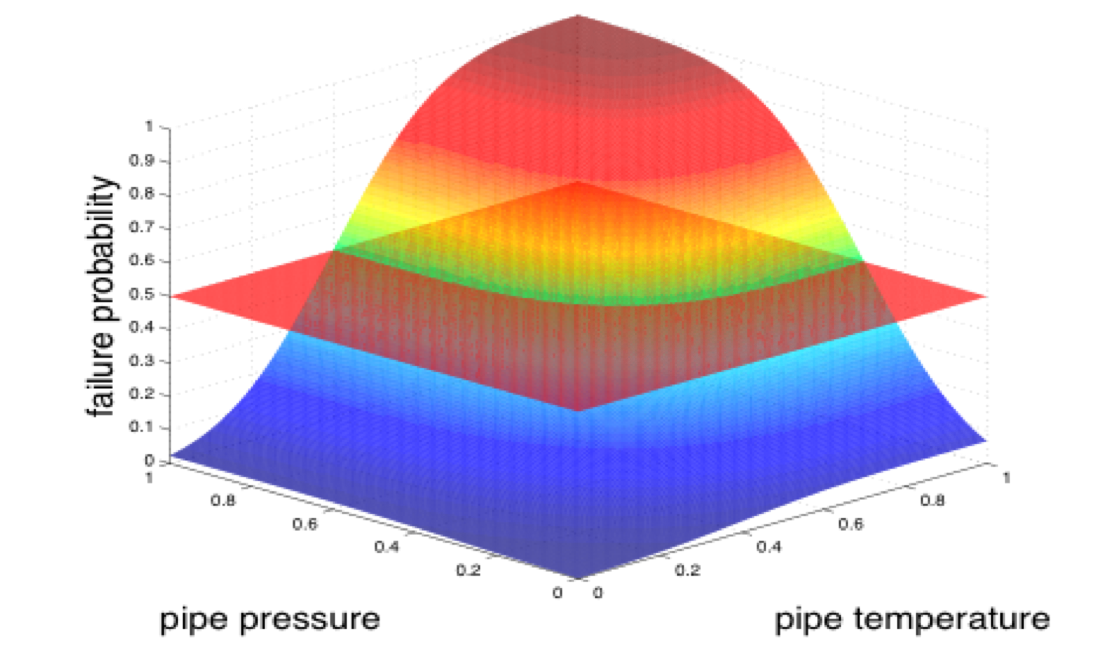
\includegraphics[width=0.5\textwidth]  {pics/NDimensionalDistributionExample.png}
  \caption{2-D CDF, function of pressure and temperature}
  \label{fig:NDDistributionExample}
\end{figure}

\subsubsection{Sampler}

The sampler is probably the most important entity in the RAVEN framework. Indeed, it performs the driving of the specific sampling strategy and, hence, determines the effectiveness of the analysis, from both an accuracy and computational point of view.  The samplers, that are available in RAVEN, can be categorized in three main classes:
\begin{itemize}
 \item Forward
 \item Dynamic Event Tree (DET)
 \item Adaptive
\end{itemize}
\paragraph{Forward Samplers} ~\\
The Forward sampler category collects all the strategies that perform the sampling of the input space without exploiting, through dynamic learning approaches, the information made available from the outcomes of calculation previously performed (adaptive sampling) and the common system evolution (patterns) that different sampled calculations can generate in the phase space (dynamic event tree).
In the RAVEN framework, several different and well-known forward samplers are available:
\begin{itemize}
\item Monte Carlo (MC)
\item Stratified based, whose most known specialization is the Latin Hyper-Cube Sampling (LHS)
\item Grid Based
\item Response Surface Design of Experiment
\item Sparse Grid
\item Factorials
\item Etc.
\end{itemize}
As already mentioned, all these sampling strategies are well known, as well as their properties. Therefore, a detailed investigation of their application is not provided.
%%%%%%%%%%%%%%%%%%%%%%%%%%%%%%%%%%%%%%%%%%%%%%%%%%%%%%%%%%%%%%%%%%%%%%%%%%%%%%%%
\paragraph{Dynamic Event Tree Samplers}~\\
In order to clarify the idea behind the Dynamic Event Tree Sampler currently available in RAVEN, a small overview is needed.
\\In technological complex systems, as nuclear power plants, an accident scenario begins with an initiating event and then evolves over time through the interaction of dynamics and stochastic events. This mutual action leads to the production of infinitely many different scenarios, which define a continuous dynamic event tree with infinite branches. At each time point, the stochastic variability of the accident outcomes is determined by a multivariate probability distribution. The PRA analysis needs an approximation to this distribution for selected consequence variables. A way to achieve this goal is an Event Tree approach. In dynamic PRA analysis, Conventional Event Tree sequences are run simultaneously starting from a single initiating event. The branches occur at user specified times and/or when an action is required by the operator and/or the system, creating a deterministic sequence of events based on the time of their occurrence. One of the disadvantages of this method is that the timing/sequencing of events and system dynamics is not explicitly accounted for in the analysis. In order to overcome these limitations a “dynamic” approach is needed. The Dynamic Event Tree (DET) technique brings several advantages, among which is the fact that it simulates probabilistic system evolution in a way that is consistent with the severe accident model. This leads to a more realistic and mechanistically consistent analysis of the system taken into consideration. The dynamic PRA, in general, and the Dynamic Event Tree methodologies in particular, are designed to take the timing of events explicitly into account, which can become very important especially when uncertainties in complex phenomena are considered. Hence, the main idea of this methodology is to let a system code determine the pathway of an accident scenario.
\\From an application point of view, a N-D grid is built on the CDF space. A single simulation is spawned and a set of triggers is added to the system code control logic. Every time a trigger gets activated (one of the CDF thresholds in the grid is violated), a new set of simulations (branches) is spawned. Each branch carries its own probability.
\\Figure \ref{fig:DETschemeExample} shows a practical example. In this particular case, it is assumed that the
probability failure of a pipe depends on the fluid pressure magnitude. Three probability thresholds are defined on
the cumulative distribution function. One simulation is spawned (0). As soon as the pressure of the fluid reaches a
value corresponding to a 33\% probability (CDF), a stop signal is sent and the framework starts two new
simulations (branches). The branch in which the system evolved to the newer condition (pipe failed, red line)
carries 33\% of the probability, while the other the complementary amount. The same procedure is repeated at
point 2.
\\Generally, not all the input space can be explored using a DET approach. For instance, usually the parameters affected by aleatory uncertainty are sampled using a dynamic event tree approach, while the ones characterized by epistemic uncertainty are sampled through ``forward'' sampling strategies.
\\As already mentioned, this strategy requires a tight interaction between the system code and the sampling driver (i.e., RAVEN framework). In addition, the system code must have a control logic capability (i.e. trigger system). For these reasons, the application of this sampling approach to a generic code needs a larger effort when compared to the other Samplers available in RAVEN. Currently, the DET is fully available for the thermal-hydraulic codes RELAP-7 and RELAP5-3D.
\\In the RAVEN framework, several different DET-based samplers are available:
\begin{itemize}
\item Dynamic Event Tree (aleatory sampling);
\item Hybrid Dynamic Event Tree (aleatory and epistemic sampling);
\item Adaptive Dynamic Event Tree (goal-oriented sampling for aleatory sampling);
\item Adaptive Hybrid Dynamic Event Tree (goal-oriented sampling for aleatory and epistemic sampling).
\end{itemize}

\begin{figure}
  \centering
  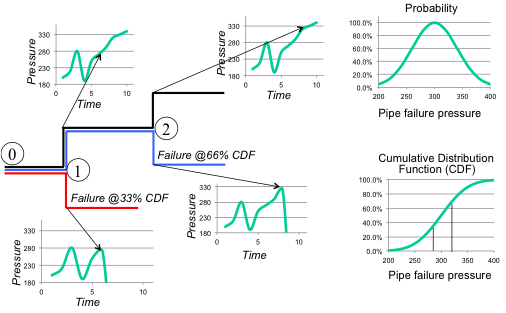
\includegraphics[width=0.7\textwidth]  {pics/DETscheme.png}
  \caption{Dynamic Event Tree simulation pattern}
  \label{fig:DETschemeExample}
\end{figure}

%%%%%%%%%%%%%%%%%%%%%%%%%%%%%%%%%%%%%%%%%%%%%%%%%%%%%%%%%%%%%%%%%%%%%%%%%%%%%%%%
\paragraph{Adaptive Samplers}~\\
A key feature available within RAVEN is the possibility to perform smart sampling (also known as adaptive sampling) as an alternative to classical ``forward'' techniques.
\\The motivation is that nuclear simulations are often computationally expensive, time-consuming, and high dimensional with respect to the number of input parameters. Thus, exploring the space of all possible simulation outcomes is unfeasible using finite computing resources. During simulation-based probabilistic risk analysis, it is important to discover the relationship between a potentially large number of input parameters and the output of a simulation using as few simulation trials as possible.
\\This is a typical context for performing adaptive sampling where a few observations are obtained from the simulation, a reduced order model (ROM) is built to represent the simulation space, and new samples are selected based on the model constructed. The ROM is then updated based on the simulation results of the sampled points. In this way, it is attempted to gain the most information possible with a small number of carefully selected sampled points, limiting the number of expensive trials needed to understand features of the system space.
\\In the RAVEN framework, several different adaptive samplers are available:
\begin{itemize}
\item Limit Surface Search;
\item Adaptive Dynamic Event Tree;
\item Adaptive Hybrid Dynamic Event Tree ;
\item Adaptive Sparse Grid;
\item Adaptive Sobol Decomposition.
\end{itemize}

\subsubsection{Models}
The Model entity, in the RAVEN environment, represents a ``connection pipeline'' between the input and the output space. The RAVEN framework does not own any physical model (i.e. it does not posses the equations needed to simulate a generic physical system, such as Navier-Stocks equations, Maxwell equations, etc.), but implements Application Program Interfaces (APIs) by which any generic model can be integrated and interrogated. The RAVEN framework provides APIs for four different model categories: Codes, Externals, Post-Processors (PPs) and Reduced Order Models (ROMs). In the following paragraphs, a brief explanation of each of this Model categories is reported.
\paragraph{Code} ~\\
The \textit{Code} model represents the communication pipe between the RAVEN framework and any system and physical code. The communication between RAVEN and any driven code is performed through the implementation of interfaces directly operated by the framework.
\\The procedure of coupling a new code/application with RAVEN is a straightforward process. The coupling is performed through a \textit{Python}  interface that interprets the information coming from RAVEN and translates them to the input of the driven code. The coupling procedure does not require modifying RAVEN itself. Instead, the developer creates a new \textit{Python} interface that is going to be embedded in RAVEN at run-time (no need to introduce hard-coded coupling statements).  This interface needs to be placed in a folder (whatever name) located in (see figure~\ref{fig:CodeInterfaceLocation}):
\begin{lstlisting}[language=bash]
 path/to/raven/distribution/raven/framework/CodeInterfaces/
\end{lstlisting}

\begin{figure}
  \centering
  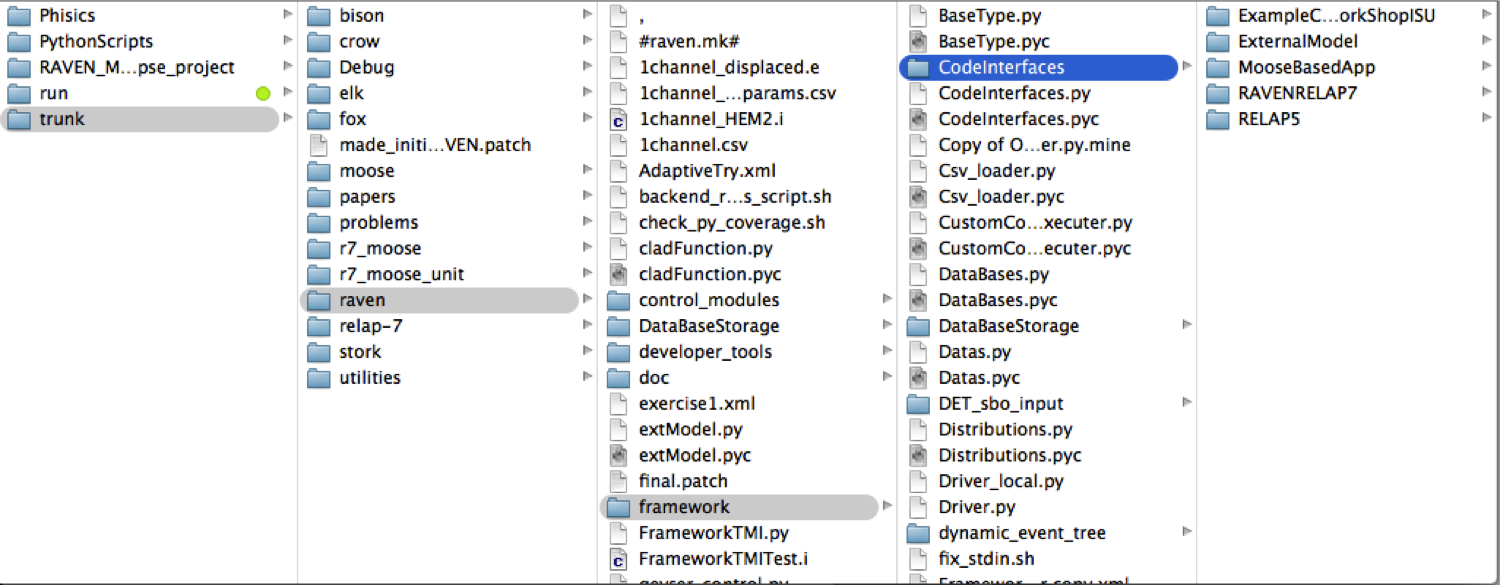
\includegraphics[width=0.8\textwidth]  {pics/CodeInterfaceLocation.png}
  \caption{Code Interface Location}
  \label{fig:CodeInterfaceLocation}
\end{figure}
At the initialization stage, RAVEN imports all the Interfaces that are contained in this directory and performs some preliminary cross-checks.
\\ If the coupled code is parallelized and/or multi-threaded, RAVEN is going to manage the system in order to optimize the computational resources in both workstations and High Performance Computing systems.
\\Currently, RAVEN has APIs for RELAP5-3D, RELAP-7, any MOOSE-based application, SASS and Modelica.
\paragraph{External Model} ~\\
The External model allows the user to create, in a \textit{Python} file (imported, at run-time, in the RAVEN framework), its own model (e.g. set of equations representing a physical model, connection to another code, control logic, etc.). This model will be interpreted/used by the framework and, at run-time, will become part of RAVEN itself.
\paragraph{Post-Processor} ~\\
The Post-Processor model represents the container of all the post-processing capabilities in the RAVEN code. This model is aimed to process the data (for example, derived from the sampling of a physical code) in order to identify representative Figure of Merits. This system has  been designed and, presently, is under heavy development by the whole RAVEN team.  Currently, the following post-processors are available:
\begin{itemize}
 \item \textit{Basic Statistics}, container of the algorithms to compute many of the most important statistical quantities. This post-processor is able to compute mean, sigma/variance, variation coefficient, skewness, kurtosis, median, percentiles and all the principal matrix quantities such as covariance, sensitivity (either leas-squared and variance weighted) and correlation matrices;
 \item \textit{Comparison Statistics}, aimed to employ validation and verification metrics;
 \item \textit{Limit Surface}, aimed to compute the limit surface in the input space (i.e. the hyper-surface that represents the boundary between the failure/success of the system);
 \item \textit{Limit Surface Integral}, intended to compute the integral of the limit surface that corresponds to the probability of failure;
  \item \textit{Safest Point}, provides the coordinates of the farthest point from the limit surface that is given as an input. The safest point coordinates are expected values of the coordinates of the farthest points from the limit surface in the space of the ``controllable'' variables based on the probability distributions of the ``non-controllable'' variables. The term ``controllable'' identifies those variables that are under control during the system operation, while the ``non-controllable'' variables are stochastic parameters affecting the system behavior randomly;
 \item \textit{External Post-Processor}, user-defined post-processor;
 \item \textit{Topological Decomposition}, aimed to compute an approximated hierarchical Morse-Smale complex which will add two columns to a data-set, performing a topological decomposition of such data-set;
 \item \textit{Data Mining}, container of all the RAVEN data mining, clustering and dimensionality reduction techniques aimed to identify dominant and common patterns in high-dimensionality data.
\end{itemize}
\paragraph{Reduced Order Model} ~\\
 As briefly mentioned, a ROM is a mathematical representation of a system, used to predict a selected output space of a physical system.
The ``training'' is a process that uses sampling of the physical model to improve the prediction capability (capability to predict the status of the system given a realization of the input space) of the ROM. More specifically, in RAVEN the Reduced Order Model is trained to emulate a high fidelity numerical representation (system codes) of the physical system. Two general characteristics of these models can be generally assumed (even if exceptions are possible):
\begin{enumerate}
   \item The higher the number of realizations in the training sets, the higher is the accuracy of the prediction performed by the reduced order model. This statement is true for most of the cases although some ROMs might be subject to the over-fitting issues. The over-fitting phenomenon is not discussed here, since its occurrence is highly dependent on the algorithm type, (and there is large number of ROM options available in RAVEN). Every time the user chooses a particular reduced order model algorithm to use, he should consult the relative literature;
   \item The smaller the size of the input domain with respect to the variability of the system response, the more likely the surrogate model will be able to represent the system output space.
\end{enumerate}
In most of the cases of interest, the information that is sought is related to defining the failure boundaries of a system with respect to perturbations in the input space. For this reason, in the development of RAVEN, it has been given priority to the introduction of a class of supervised learning algorithms, which are usually referred to as classifiers. A classifier is a reduced order model that is capable of representing the system behavior through a binary response (failure/success).
\\The first class of classifier introduced has been the Support Vector Machines (SVMs) [reference] with several different kernels (polynomial of arbitrary integer order, radial basis function kernel, sigmoid) followed by a nearest-neighbor based classification using a K-D tree search algorithm. Currently, RAVEN supports around 40 different ROM methodologies. All these supervised learning algorithms have been imported via an API from the scikit-learn [reference] library. In addition, the N-Dimensional spline and the inverse weight methods, that are currently available for the interpolation of N-Dimensional PDF/CDF, can also be used as ROMs.
\subsubsection{Simulation Environment}
RAVEN is perceived by the user as a pool of tools and data. Any action in which the tools are applied to the data is considered a calculation ``step'' in the RAVEN environment. Simplistically, a ``step'' can be seen as a \textbf{transfer function} between the input and output space through a Model (e.g. Code, External, ROM or Post-Processor). One of the most important step in the RAVEN framework is called ``multi-run'', that is aimed to handle calculations that involve multiple runs of a driven code (sampling strategies). Firstly, the RAVEN input file associates the variables to a set of PDFs and to a sampling strategy. The ``multi-run'' step is used to perform several runs in a block of a model (e.g. in a MC sampling).
\begin{figure}[ht]
  \centering
  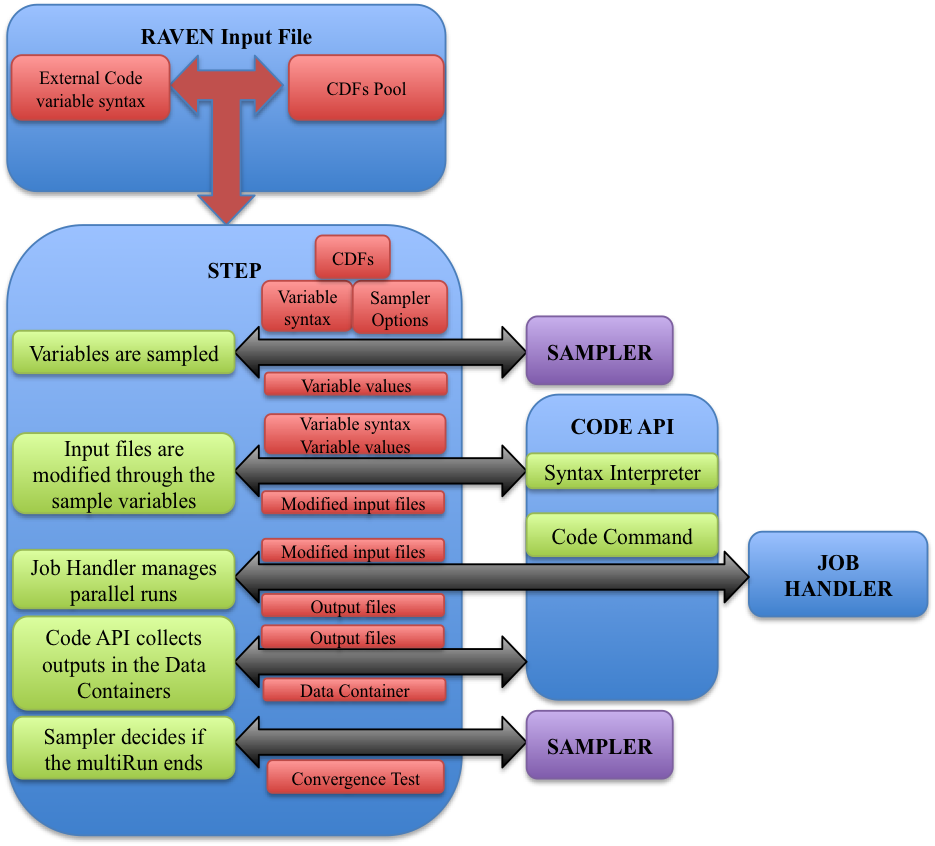
\includegraphics[width=0.8\textwidth]  {pics/MultiRunCalculationFlow.png}
  \caption{Calculation flow for a multi-run sampling}
  \label{fig:multiRun}
\end{figure}
At the beginning of each sub sequential run, the sampler provides the new values of the variables to be perturbed. The code API places those values in the input file. At this point, the code API generates the run command and asks to be queued by the job handler. The job handler manages the parallel execution of as many runs as possible within a user prescribed range and communicates with the step controller when a new set of output files are ready to be processed. The code API receives the new input files and collects the data in the RAVEN internal format. The sampler is queried to assess if the sequence of runs is ended, if not, the step controller asks for a new set of values from the sampler and the sequence is restarted as described in Figure~\ref{fig:multiRun}.
The job handler is currently capable to run different run instances of the code in parallel and can also handle codes that are multi-threaded or using any form of parallel implementation.
RAVEN also has the capability to plot the simulation outcomes while the set of sampling is performed and to store the data for later recovery.

\section{Raven Input Structure}
The RAVEN code does not have a fixed calculation flow, since all of its basic
objects can be combined in order to create a user-defined calculation flow.
%
Thus, its input (XML format) is organized in different XML blocks, each with a
different functionality.
%
The main input blocks are as follows:
\begin{itemize}
  \item \textbf{\textless Simulation\textgreater}: The root node containing the
  entire input, all of
  the following blocks fit inside the \emph{Simulation} block.
  %
  \item \textbf{\textless RunInfo\textgreater}: Specifies the calculation
  settings (number of parallel simulations, etc.).
  %
  \item \textbf{\textless Files\textgreater}: Specifies the files to be
  used in the calculation.
  %
  \item \textbf{\textless Distributions\textgreater}: Defines distributions
  needed for describing parameters, etc.
  %
  \item \textbf{\textless Samplers\textgreater}: Sets up the strategies used for
  exploring an uncertain domain.
  %
  \item \textbf{\textless Functions\textgreater}: Details interfaces to external
  user-defined functions and modules.
  %
  \item \textbf{\textless Models\textgreater}: Specifies codes, ROMs,
  post-processing analysis, etc.
  %
  the user will be building and/or running.
  %
  \item \textbf{\textless Steps\textgreater}: Combines other blocks to detail a
  step in the RAVEN workflow including I/O and computations to be performed.
  %
  \item \textbf{\textless DataObjects\textgreater}: Specifies internal data objects
  used by RAVEN.
  %
  \item \textbf{\textless Databases\textgreater}: Lists the HDF5 databases used
  as input/output to a
  RAVEN run.
  %
  \item \textbf{\textless OutStreamManager\textgreater}: Visualization and
  Printing system block.
  %
\end{itemize}

Each of these blocks are explained in dedicated sections in the following
chapters.
%
\subsection{Comments}
Comments may be included in the RAVEN input using standard XML comments,
using \verb|<!--| and \verb|-->| as shown in the example below.
\begin{lstlisting}[style=XML]
<Simulation>
  ...
  <!-- An Example Comment -->
  <Samplers>
  ...
\end{lstlisting}
Comments may be placed anywhere \emph{except} before the \xmlNode{Simulation}
node or after the \xmlNode{/Simulation} node.
%
Comments outside the root node will cause errors in maintaining input file
compatability.
%
Additionally, comments must completely surround any nodes they comment out.
%
Comments are intended to completely remove blocks of code, or to add readability.
%
For instance, the following is INCORRECT usage:
\begin{lstlisting}[style=XML]
  <!--<Assembler> -->
  <!--</Assembler> -->
\end{lstlisting}
%
and the following is compatible usage for a code block:
%
\begin{lstlisting}[style=XML]
  <!--<Samplers>
    <Monte Carlo name='mc'>
      ...
    </Monte Carlo>
    ...
  </Samplers> -->
\end{lstlisting}


\subsection{Verbosity}
Each block within RAVEN also makes use of a \xmlAttr{verbosity} system,
which allows a user to control the level of output to the user interface.
These settings are declared globally as attributes in the \xmlNode{Simulation} node,
and locally in each block.  The verbosity levels are
\begin{itemize}
\item \xmlString{silent} - Only simulation-breaking errors are displayed.
\item \xmlString{quiet} - Errors as well as warnings are displayed.
\item \xmlString{all} (default) - Errors, warnings, and messages are displayed.
\item \xmlString{debug} - For developers. All errors, warnings, messages, and debug messages are displayed.
\end{itemize}
Examples of verbosity usage are included in many examples throughout this manual.

At the \xmlNode{Simulation} node, global variables can be set, including \xmlAttr{verbosity}.  In addition, the
attribute \xmlAttr{printTimeStamps} can be used to either enable or disable prepending RAVEN output with time stamps
by setting it to \xmlString{true} or \xmlString{false}.


\subsection{External Input Files}
The \xmlNode{ExternalXML} node defines external input file (XML format) that can be used to replace any XML nodes 
under \xmlNode{Simulation} in the RAVEN input file. This node allows a user to load any external input file that contains 
the required XML nodes into the RAVEN input file. Each \xmlNode{ExternalXML} node has the following attributes:
\begin{itemize}
\item \xmlAttr{node}, \xmlDesc{required string attribute}, user-defined XML node of RAVEN input file. 
\item \xmlAttr{xmlToLoad}, \xmlDesc{required string attribute}, file name with its absolute or relative path. Note: if a 
relative path is specified, it must be relative with respect to the RAVEN input file.
\end{itemize}
%
For example, if the file \texttt{Models.xml} contain the required RAVEN input XML node \xmlNode{Models}, 
the RAVEN input file might appear as: 
%
\begin{lstlisting}[style=XML,morekeywords={node,xmlToLoad}]  
<Simulation>
  ...
  <Steps>
    ...
  </Steps>
  ...
  <ExternalXML node='Models' xmlToLoad='external_input/Models.xml'/>
  ...
</Simulation>
\end{lstlisting}
%
Another example, if the file \texttt{MultiRun.xml} contain the required RAVEN input XML node \xmlNode{MultiRun} 
under node \xmlNode{Steps}, the RAVEN input file might appear as:
\begin{lstlisting}[style=XML,morekeywords={node,xmlToLoad}]  
<Simulation>
  ...
  <Steps>
    ...
    <ExternalXML node='MultiRun' xmlToLoad='external_input/MultiRun.xml'/>
    ...
  </Steps>
  ...
</Simulation>
\end{lstlisting}

\section{Manual Formats}
In order to highlight some parts of the manual having a particular meaning (input structure, examples, terminal commands, etc.), specific formats have been used. This section provides the formats with a specific meaning:
\begin{itemize}
\item \textbf{\textit{Python Coding:}}
\begin{lstlisting}[language=python]
class AClass():
  def aMethodImplementation(self):
    pass
\end{lstlisting}
\item \textbf{\textit{XML input example:}}
\begin{lstlisting}[style=XML,morekeywords={anAttribute}]
<MainXMLBlock>
  ...
  <aXMLnode name='anObjectName' anAttribute='aValue'>
     <aSubNode>body</aSubNode>
  </aXMLnode>
  <!-- This is  commented block -->
  ...
</MainXMLBlock>
\end{lstlisting}
\item \textbf{\textit{Bash Commands:}}
\begin{lstlisting}[language=bash]
cd trunk/raven/
./raven_libs_script.sh
cd ../../
\end{lstlisting}
\end{itemize}


\section{Manual Structure}
This manual is intended to provide an overview of the RAVEN capabilities through the explanation of multiple commented examples.
To speed up the learning process, the examples are organized in an ascending complexity order, from simple data manipulation and visualization to
full Probabilistic Risk Assessment and Uncertainty Quantification analysis. In addition, each example is followed by a brief explanation of the theoretical background of the methods that have been used.
\\ It is important to notice that this document is intended to be consulted in conjunction with the user manual ~\cite{RAVENuserManual}.
\\To generalize the examples to any driven software, a simple \texttt{Python} code (conventionally called \textbf{AnalyticBateman}) has been developed (located at ``\textit{doc/user\textunderscore guide/ravenInputs/physicalCode}''). It solves a system of ordinary differential equations (ODEs), of the form:

\begin{equation}
\begin{dcases}
\frac{\mathrm{d} \mathbf{X}}{\mathrm{d} t} = \mathbf{S}-\mathbf{L} \\
 \mathbf{X}(t=0)= \mathbf{X_{0}}
\end{dcases}
\end{equation}
   where:
  \begin{itemize}
     \item $\mathbf{X_{0}}$, initial conditions
     \item $\mathbf{S}$, source terms
     \item $\mathbf{L}$, loss terms
   \end{itemize}

For example, this  code is able to solve a system of equations as follows:
\begin{equation}
  \begin{dcases}
   \frac{\mathrm{d} x_{1}}{\mathrm{d} t} = \phi (t)\times \sigma_{x_{1}}-\lambda_{x_{1}} \\
   \frac{\mathrm{d} x_{2}}{\mathrm{d} t} = \phi (t)\times \sigma_{x_{2}}-\lambda_{x_{2}}+x_{1}(t)\times\lambda_{x_{1}} \\
    x_{1}(t=0)= x_{1}^{0} \\
    x_{2}(t=0)= 0.0
  \end{dcases}
\end{equation}

The input of the \textbf{AnalyticBateman} code is in XML format.
For example, the following is the reference input for a system of 4 Ordinary Differential Equations (ODEs)
that is going to be used for all the examples reported in this manual.  For some examples, the number of
calculated steps might be adjusted for time of calculation (\xmlNode{timeSteps}); however, the operation is
similar for exemplary purposes.

\xmlExample{framework/user_guide/physicalCode/analyticalbateman/Input.xml}{AnalyticalBateman}
The code outputs the time evolution of the 4 variables ($A,B,C,D$) in a CSV file, producing the following output:
\begin{table}[ht]
\centering
\caption{Reference case sample results.}
\label{referenceResults}
\begin{tabular}{lllll}
\textbf{time} & \textbf{A}     & \textbf{C}     & \textbf{B}    & \textbf{D}     \\
0                  & 1.0                       & 1.0                       & 1.0                     & 1.0           \\
2880000.0   & 0.983434738239 & 0.977851848235 & 1.01011506729 & 1.01013172275 \\
5760000.0   & 0.967143884376 & 0.956202457404 & 1.01936231677 & 1.02036100400   \\
8640000.0   & 0.951122892771 & 0.935040450532 & 1.02777406275 & 1.03067925987 \\
10368000.0 & 0.941637968936 & 0.922572556179 & 1.03243314106 & 1.03690947068 \\
12096000.0 & 0.932247632016 & 0.910273757371 & 1.03680933440 & 1.04316700086 \\
13824000.0 & 0.922950938758 & 0.898141730426 & 1.04090912054 & 1.04945015916 \\
15552000.0 & 0.913746955315 & 0.886174183908 & 1.04473885709 & 1.05575729317 \\
17280000.0 & 0.904634757153 & 0.874368858183 & 1.04830478357 & 1.06208678854 \\
20736000.0 & 0.886682064542 & 0.851235986899 & 1.05466958557 & 1.07480659230  \\
24192000.0 & 0.869085647400 & 0.828725658721 & 1.06005115510 & 1.08759739100   \\
27648000.0 & 0.851838435355 & 0.806820896763 & 1.06449535534 & 1.10044757060  \\
31104000.0 & 0.834933498348 & 0.785505191756 & 1.06804634347 & 1.11334606143 \\
34560000.0 & 0.818364043850 & 0.764762489077 & 1.07074662835 & 1.12628231792
\end{tabular}
\end{table}

RAVEN is able to directly retrieve CSV files as output; for this reason, the \textit{\textbf{GenericInterface}} (see ~\cite{RAVENuserManual}-Chapter ``Existing Interfaces'') is used to drive the code.

\section{Run a Single Instance of a Code and Load the Outputs}
The simplest exercise that can be performed is to run the driven code (\textbf{AnalyticBateman}  in our example), loading the results of a single run into RAVEN, printing and plotting some variables.
\\ As detailed in the RAVEN user manual (~\cite{RAVENuserManual}-Chapters ``DataObjects''  and ``Databases'') and in Chapter~/ref{sub:EntitiesAndFlow} RAVEN uses two classes of objects to store the data coming from a driven code (outputs):
\begin{itemize}
  \item \textbf{DataObjects}: The DataObjects represent the preferred way to transfer the information coming from a
   Model (the driven code, in this case) to all the other RAVEN systems (e.g. Out-Stream system, Reduced Order Modeling
   component, etc.).
  \item \textbf{Databases}.
\end{itemize}

As esaly inferable from the user manual (~\cite{RAVENuserManual}-Chapter ``OutStream''), the DataObjects can be exported into a CSV file and plotted (2-D and 3-D plots) linking them into the OutStream system.
\\ The following subsections report examples on how to use these systems running a single instance of the driven code.
\subsection{Single Run using the OutStream system for printing and create basic plots}
\label{sub:SingleRunBasicPlots}
 In this Section, the user can learn how to use RAVEN to run a single instance of a driven code, plotting and printing the
 results.
 \\ The goal of this Section is to learn how to:
 \begin{enumerate}
   \item Set up a simple RAVEN input for running a driven code;
   \item Load the output of the code into the RAVEN DataObjects system;
   \item Print out what contained in the DataObjects;
   \item Generate basic plots of the code results.
\end{enumerate}
In order to accomplish these tasks, the following RAVEN \textbf{Entities} (XML blocks in the input files) are needed:
 \begin{enumerate}
   \item \textbf{\textit{RunInfo}}:
\begin{lstlisting}[style=XML,morekeywords={arg,extension,pauseAtEnd,overwrite}]
    <RunInfo>
      <Sequence>Single, write-History</Sequence>
      <WorkingDir>SectionVI.I</WorkingDir>
      <batchSize>1</batchSize>
    </RunInfo>
\end{lstlisting}
   As reported in Section~\ref{sub:EntitiesAndFlow}, the \textit{RunInfo} \textbf{Entity} is intended to set up the analysis
   that the user wants to perform. In this specific case, two steps (\xmlNode{Sequence}) are going to be sequentially run
   using a single processor (\xmlNode{batchSize}).

   \item \textbf{\textit{Files}}:
\begin{lstlisting}[style=XML,morekeywords={arg,extension,pauseAtEnd,overwrite}]
  <Files>
    <Input name="referenceInput.xml" type="input">referenceInput.xml</Input>
  </Files>
\end{lstlisting}
   Since the driven code uses a single input file, in this Section the original input is placed. As described in the user manual~\cite{}
   the attribute  \xmlAttr{name} represents the alias that is going to be used in all the other input blocks in order to
   refer to this file.
   \item \textbf{\textit{Models}}:
\begin{lstlisting}[style=XML,morekeywords={arg,extension,pauseAtEnd,overwrite}]
   <Models>
      <Code name="testModel" subType="GenericCode">
        <executable>
      ../physicalCode/analyticalbateman/AnalyticalDplMain.py
        </executable>
        <clargs arg="python" type="prepend"/>
        <clargs arg="" extension=".xml" type="input"/>
        <clargs arg="" extension=".csv" type="output"/>
        <prepend>python</prepend>
      </Code>
    <Models>
\end{lstlisting}
  Since the driven code already dumps its outputs in CSV format, there is no need to create
  an ad-hoc code interface and the GenericCode interface can be directly used. In additiom, since the \textbf{AnalyticBateman} code
  is written in \texttt{Python}, it is necessary to specify that the code needs to be run pre-pending the expression ``\texttt{Python}''.
   \item \textbf{\textit{DataObjects}}:
\begin{lstlisting}[style=XML,morekeywords={arg,extension,pauseAtEnd,overwrite}]
  <DataObjects>
    <PointSet name="pointValues">
      <Input>InputPlaceHolder</Input>
      <Output>A,B,C,D</Output>
    </PointSet>
    <HistorySet name="history">
        <Input>InputPlaceHolder</Input>
        <Output>A,B,C,D,time</Output>
    </HistorySet>
  </DataObjects>
\end{lstlisting}
  Int this block, two \textit{DataObjects} are defined: 1) PointSet named ``pointValues'', 2) HistorySet named ``history''.
  Note that a special keyword is inputted in the \xmlNode{Input} node. This keyword is used when a \textit{DataObjects}  \textbf{Entity} needs to be constructed without any linking with respect to the input space. Indeed, in
  this case, the model input space is not perturbed though a sampling strategies; the code is executed through the original
   input file   (``referenceInput.xml''). In the \xmlNode{Output} node all the requested variables are inputted.
   \item \textbf{\textit{OutStreamManager}}:
\begin{lstlisting}[style=XML,morekeywords={arg,extension,pauseAtEnd,overwrite}]
  <OutStreamManager>
    <Print name="pointValues">
      <type>csv</type>
      <source>pointValues</source>
    </Print>
    <Print name="history">
        <type>csv</type>
        <source>history</source>
    </Print>
    <Plot dim="2" name="historyPlot" overwrite="false" verbosity="debug">
        <plotSettings>
            <plot>
                <type>line</type>
                <x>history|Output|time</x>
                <y>history|Output|A</y>
                <color>blue</color>
            </plot>
            <plot>
                <type>line</type>
                <x>history|Output|time</x>
                <y>history|Output|B</y>
                <color>red</color>
            </plot>
            <plot>
                <type>line</type>
                <x>history|Output|time</x>
                <y>history|Output|C</y>
                <color>yellow</color>
            </plot>
            <plot>
                <type>line</type>
                <x>history|Output|time</x>
                <y>history|Output|D</y>
                <color>black</color>
            </plot>
            <xlabel>time (s)</xlabel>
            <ylabel>evolution (kg)</ylabel>
        </plotSettings>
        <actions>
            <how>png,screen</how>
            <title>
                <text> </text>
            </title>
        </actions>
    </Plot>
  </OutStreamManager>
\end{lstlisting}
  In this block, both the Out-Stream types are constructed:
  \begin{itemize}
    \item \textit{Print}:
     \begin{itemize}
       \item named ``pointValues'' connected with the \textit{DataObjects} \textbf{Entity} ``pointValues''
                (\xmlNode{source})
       \item named ``history'' connected with the \textit{DataObjects} \textbf{Entity} ``history'' (\xmlNode{source})
     \end{itemize}
      When this objects get used, all the information contained in the linked  \textit{DataObjects} are going
    to be dumped in CSV files (\xmlNode{type}).
    \item \textit{Plot}: a single \xmlNode{Plot} \textbf{Entity} is defined, containing the line plots of the 4 output variables
    ($A,B,C,D$) in the same figure. This object is going to generate a PNG file and an interactive Plot on
    the screen.
  \end{itemize}
   \item \textbf{\textit{Steps}}:
\begin{lstlisting}[style=XML,morekeywords={arg,extension,pauseAtEnd,overwrite}]
  <Steps>
    <SingleRun name="Single">
      <Input   class="Files"                        type="input">referenceInput.xml</Input>
      <Model  class="Models"                    type="Code">testModel</Model>
      <Output class="DataObjects"            type="PointSet">pointValues</Output>
      <Output class="DataObjects"            type="HistorySet">history</Output>
      <Output class="OutStreamManager" type="Print">pointValues</Output>
    </SingleRun>
    <IOStep name="writeHistory" pauseAtEnd="True">
        <Input    class="DataObjects"            type="HistorySet">history</Input>
        <Output class="OutStreamManager" type="Print">history</Output>
        <Output class="OutStreamManager" type="Plot">historyPlot</Output>
    </IOStep>
  </Steps>
\end{lstlisting}
 %%%%%%%%%%%%%%%%%%%%%%%%%%%%%%%%%%%%%%%%%%%%%%%%%%%%%%%%%%
 %figure history
 \begin{figure}[h!]
  \centering
  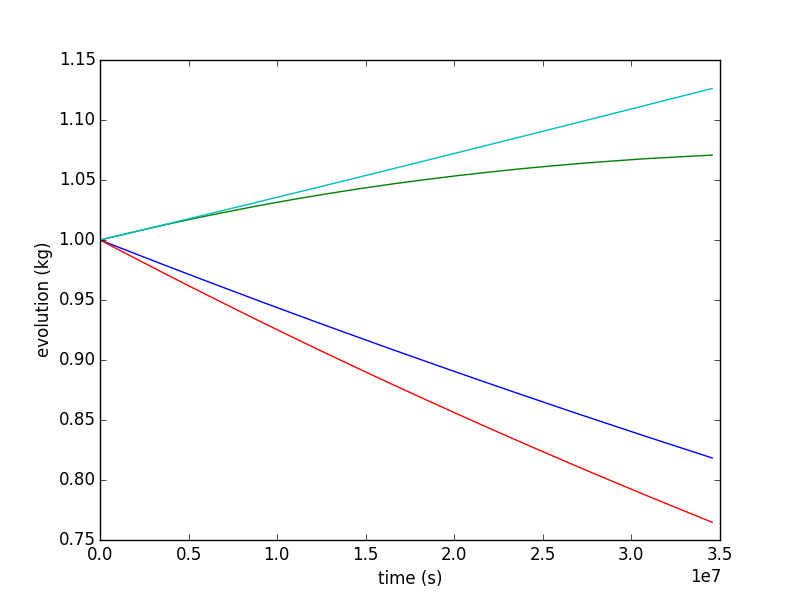
\includegraphics[scale=0.7]{pics/1-historyPlot_line-line-line-line.png}
  \caption{Plot of the history for variables $A,B,C,D$.}
  \label{fig:historyPlotLine}
 \end{figure}
 %%%%%%%%%%%%%%%%%%%%%%%%%%%%%%%%%%%%%%%%%%%%%%%%%%%%%%%%%%
   Finally, all the previously defined \textbf{Entities} can be combined in the \xmlNode{Steps} block. Thus,
   two \xmlNode{Steps} have been inputted:
   \begin{itemize}
     \item \xmlNode{SingleRun} named ``Single'', used to run the single instance of the driven code and collect
     the outputs in the two \textit{DataObjects}. In addition, it can be seen that an additional object has been
     placed among the \xmlNode{Output}(s). Indeed, an  \textit{OutStreamManager} can be an \xmlNode{Output} in
     any Step type (as long as the linked \textit{DataObjects} plays a whatever role in the Step)
     \item  \xmlNode{IOStep} named ``writeHistory'', used to 1) dump the ``history'' \textit{DataObjects}
     \textbf{Entity} in a CSV file and 2) plot the data in the PNG file and on the screen.
   \end{itemize}
\end{enumerate}
 Tables~\ref{historyVI.I} and \ref{pointValuesVI.I} show the results dumped by the OutStreams \textit{Print}.
 As previously mentioned, Figure~\ref{fig:historyPlotLine} reports the four plots (four variables) drawn in the same picture.
 % table history set
\begin{table}[h!]
\centering
\caption{``history'' HistorySet CSV output file.}
\label{historyVI.I}
\begin{tabular}{|c|c|c|c|c|}
\hline
\textbf{A}                        & \textbf{C}                       & \textbf{B}                       & \textbf{D}                       & \textbf{time}                 \\ \hline
1                                 & 1                                & 1                                & 1                                & 0                             \\ \hline
0.983434738                       & 0.977851848                      & 1.010115067                      & 1.010131723                      & 2880000                       \\ \hline
0.967143884                       & 0.956202457                      & 1.019362317                      & 1.020361004                      & 5760000                       \\ \hline
0.951122893                       & 0.935040451                      & 1.027774063                      & 1.03067926                       & 8640000                       \\ \hline
0.941637969                       & 0.922572556                      & 1.032433141                      & 1.036909471                      & 10368000                      \\ \hline
0.932247632                       & 0.910273757                      & 1.036809334                      & 1.043167001                      & 12096000                      \\ \hline
0.922950939                       & 0.89814173                       & 1.040909121                      & 1.049450159                      & 13824000                      \\ \hline
0.913746955                       & 0.886174184                      & 1.044738857                      & 1.055757293                      & 15552000                      \\ \hline
0.904634757                       & 0.874368858                      & 1.048304784                      & 1.062086789                      & 17280000                      \\ \hline
0.886682065                       & 0.851235987                      & 1.054669586                      & 1.074806592                      & 20736000                      \\ \hline
0.869085647                       & 0.828725659                      & 1.060051155                      & 1.087597391                      & 24192000                      \\ \hline
\multicolumn{1}{|l|}{0.851838435} & \multicolumn{1}{l|}{0.806820897} & \multicolumn{1}{l|}{1.064495355} & \multicolumn{1}{l|}{1.100447571} & \multicolumn{1}{l|}{27648000} \\ \hline
\multicolumn{1}{|l|}{0.834933498} & \multicolumn{1}{l|}{0.785505192} & \multicolumn{1}{l|}{1.068046343} & \multicolumn{1}{l|}{1.113346061} & \multicolumn{1}{l|}{31104000} \\ \hline
\multicolumn{1}{|l|}{0.818364044} & \multicolumn{1}{l|}{0.764762489} & \multicolumn{1}{l|}{1.070746628} & \multicolumn{1}{l|}{1.126282318} & \multicolumn{1}{l|}{34560000} \\ \hline
\end{tabular}
\end{table}
% table point set
\begin{table}[h!]
\centering
\caption{``pointValues'' PointSet CSV output file.}
\label{pointValuesVI.I}
\begin{tabular}{|c|c|c|c|c|}
\hline
\textbf{InputPlaceHolder} & \textbf{A}    & \textbf{C}     & \textbf{B}    & \textbf{D}    \\ \hline
0.0                       & 0.81836404385 & 0.764762489077 & 1.07074662835 & 1.12628231792 \\ \hline
\end{tabular}
\end{table}


\subsection{Single Run using the OutStream System to Sub-plot and Selectively print.}
This Section shows how to use RAVEN to create sub-plots (multiple plots in the same figure) and
how to select only some variable from the \textit{DataObjects} in the \textit{Print} OutStream.
 \\ The goals of this Section are about learning how to:
 \begin{enumerate}
   \item Print out what contained in the DataObjects, selecting only few variables
   \item Generate sub-plots (multiple plots in the same figure) of the code results
\end{enumerate}

To accomplish these tasks, the \textit{OutStreamManager} \textbf{Entity} in the input defined in the previous Section (~\ref{sub:SingleRunBasicPlots}) needs to be modified as follows:
\begin{enumerate}
   \item \textbf{\textit{Print}}:
   \begin{lstlisting}[style=XML,morekeywords={arg,extension,pauseAtEnd,overwrite}]
    <Print name="pointValues">
      <type>csv</type>
      <source>pointValues</source>
      <what>Output</what>
    </Print>
    <Print name="history">
        <type>csv</type>
        <source>history</source>
        <what>Output|A,Output|D</what>
    </Print>
   \end{lstlisting}
   With respect to the \textit{Print} nodes defined in the previous Section (~\ref{sub:SingleRunBasicPlots}), it can
   be noticed that an additional node has been added: \xmlNode{what}. The \textit{Print} \textbf{Entity}
   ``pointValues'' is going to extract and dump only the variables that are part of the Output space
   ($A,B,C,D$ and not $InputPlaceHolder$).  The \textit{Print} \textbf{Entity} ``history'' is instead going to print
   the Output space variables $A$ and $D$.

   \item \textbf{\textit{Plot}}:
   \begin{lstlisting}[style=XML,morekeywords={arg,extension,pauseAtEnd,overwrite}]
    <Plot dim="2" name="historyPlot" overwrite="false" verbosity="debug">
        <plotSettings>
            <gridSpace>2 2</gridSpace>
            <plot>
                <type>line</type>
                <x>history|Output|time</x>
                <y>history|Output|A</y>
                <color>blue</color>
                <gridLocation>
                  <x>0</x>
                  <y>0</y>
                </gridLocation>
            </plot>
            <plot>
                <type>line</type>
                <x>history|Output|time</x>
                <y>history|Output|B</y>
                <color>red</color>
                <gridLocation>
                    <x>1</x>
                    <y>0</y>
                </gridLocation>
            </plot>
            <plot>
                <type>line</type>
                <x>history|Output|time</x>
                <y>history|Output|C</y>
                <color>yellow</color>
                <gridLocation>
                    <x>0</x>
                    <y>1</y>
                </gridLocation>
            </plot>
            <plot>
                <type>line</type>
                <x>history|Output|time</x>
                <y>history|Output|D</y>
                <color>black</color>
                <gridLocation>
                    <x>1</x>
                    <y>1</y>
                </gridLocation>
            </plot>
            <xlabel>time (s)</xlabel>
            <ylabel>evolution (kg)</ylabel>
        </plotSettings>
        <actions>
            <how>png,screen</how>
            <title>
                <text> </text>
            </title>
        </actions>
    </Plot>
\end{lstlisting}
 Note that the  \textit{Plot} \textbf{Entity} does not differ much with respect to the one in
 Section~\ref{sub:SingleRunBasicPlots}: 1) the additional sub-node \xmlNode{gridSpace}  has been added.
 This node is needed to define how the figure needs to be partitioned (discretization of the grid). In this case
 a 2 by 2 grid is requested. 2) in each \xmlNode{plot} the node \xmlNode{gridLocation} is placed in
 order to specify in which position the relative plot needs to be placed. For example, in the following grid
 location, the relative plot is going to be placed at the bottom-right corner.
  \begin{lstlisting}[style=XML,morekeywords={arg,extension,pauseAtEnd,overwrite}]
   <gridLocation>
      <x>1</x>
      <y>1</y>
   </gridLocation>
   \end{lstlisting}
 \end{enumerate}
The CSV tables generated by the \textit{Print} \textbf{Entities} are not reported, since the only differences with respect to Tables ~\ref{historyVI.I} and ~\ref{pointValuesVI.I} are related to the number of columns (variables)
dumped out.
\\Figure~\ref{fig:historySubPlotLine} reports the four plots (four variables) drawn in the same picture.
 %figure history sublots
 \begin{figure}[h!]
  \centering
  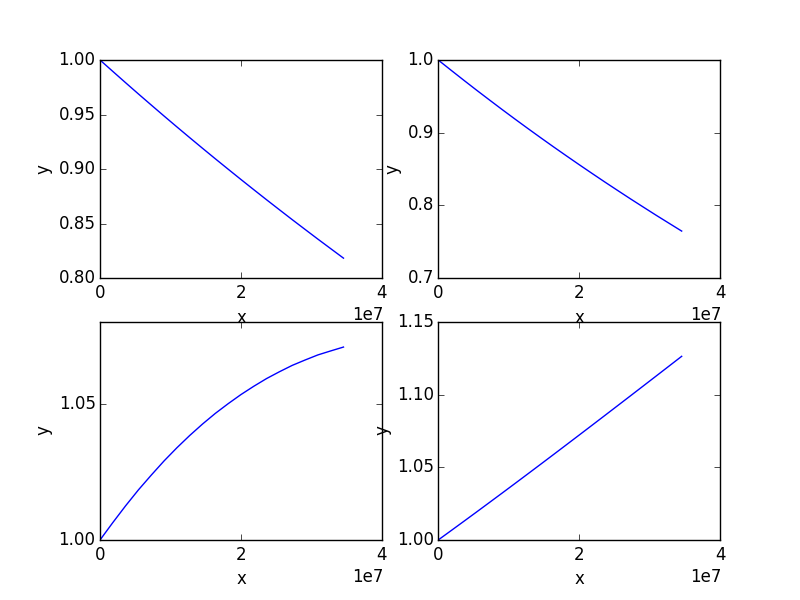
\includegraphics[scale=0.7]{pics/1-historyPlot_line-line-line-line-subPlots.png}
  \caption{Subplot of the history for variables $A,B,C,D$.}
  \label{fig:historySubPlotLine}
 \end{figure}


\section{Forward Sampling Strategies}
\label{sec:forwardSamplingStrategies}
In order to perform uncertainty quantification (UQ) and dynamic
probabilistic risk assessment (D-PRA),
a sampling strategy needs to be employed. The sampling strategy aims to
perturb the input space (domain of the uncertainties) in order to explore
the response of a complex system in relation to selected Figures of 
Merits (FOMs). 
\\The most widely used strategies to perform UQ and PRA are generally
collected into the category that, in RAVEN, is called \textit{\textbf{Forward}} samplers. The \textit{\textbf{Forward}} sampler category collects all the strategies that perform the sampling of the input space without exploiting, through learning approaches, the information made available from the outcomes of evaluation previously performed (adaptive sampling) and the common system evolution (patterns) that different sampled calculations can generate in the phase space (Dynamic Event Tree). 
\\As mentioned in Section~\ref{par:ForwardSamplers}, RAVEN has
different \textit{\textbf{Forward}} samplers:
\begin{itemize}
  \item \textit{Monte-Carlo};
  \item \textit{Grid-based};
  \item \textit{Stratified} and its specialization, i.e. \textit{Latin Hyper Cube}.
\end{itemize}
In addition, RAVEN posses advanced \textit{\textbf{Forward}} sampling strategies that:
\begin{itemize}
  \item build a grid in the input space selecting evaluation points 
  based on characteristic quadratures as part of stochastic collocation 
  for generalized polynomial chaos method (\textit{Sparse 
  Grid Collocation} sampler);
  \item use high-density model reduction (HDMR) a.k.a. Sobol 
  decomposition to approximate a function as the sum of increasing-
  complexity interactions (\textit{Sobol} sampler).
\end{itemize} 
In the following subsections, the theory behind these sampling 
methodologies are going to be explained by way of applied RAVEN 
examples.
%%%%%%%%%%%%%%%%%%%%%%%%%
%%%%%%%%  MONTE-CARLO %%%%%%%% 
%%%%%%%%%%%%%%%%%%%%%%%%%
\subsection{Monte-Carlo}
\label{sub:MC}
The Monte-Carlo method is probably one of the most used methodologies in several disciplines. In this section, a brief theoretical 
background is reported. In addition,it is shown how to employ this methodology with RAVEN.
\subsubsection{Monte-Carlo}
\label{subsub:MCtheory}
The Monte-Carlo method approximates an expectation by the sample mean of a function of 
simulated random variables. It is based on the laws of large numbers in order to approximate expectations. 
In order words, it approximates the average response of multiple FOMs 
relying on multiple random sampling of the input space. 
\\Let's consider a random variable (eventually multidimensional) $X$ having probability mass function or probability density function $pdf_{X}(x)$,
which is greater than zero on a set of values $\chi$. Then the expected value of a function $f$ of $X$ is as follows:
\begin{equation}
\begin{matrix}
\mathbb{E}(f(X)) =\sum_{x \in \chi} f(x)pdf_{X}(x) & \text{if} X \, discrete \\ 
\\ 
\mathbb{E}(f(X)) =\int_{x \in \chi} f(x)pdf_{X}(x) & \, \text{if} X \, \, continuous
\end{matrix}
\end{equation}
Let's now consider $n$ samples of $X$, $(x_{1},...,x_{n})$, and compute the mean of $f(x)$ over the samples. This computation represents the Monte-Carlo estimate:
\begin{equation}
  \mathbb{E}(f(X)) \approx   \widetilde{f}_{n}(x) = \frac{1}{n} \sum_{i=1}^{n} f(x_{i})  
\end{equation}
If $\mathbb{E}(f(X))$ exists, then the law of large numbers determines that for any arbitrarily small $\varepsilon$:
\begin{equation}
  \lim_{n\rightarrow \, \infty} P( \left | \widetilde{f}_{n}(X) - \mathbb{E}(f(X))  \right |\geq \varepsilon) = 0
\end{equation}
The above equation suggests that as $n$ gets larger, then the probability that $\widetilde{f}_{n}(X)$ deviates 
from the $\mathbb{E}(f(X))$ becomes smaller. In other words, more samples are spooned, more closer the Monte-Carlo estimate of $X$ gets to the real value.
\\In addition $\widetilde{f}_{n}(X)$ represent an unbiased estimate for $\mathbb{E}(f(X))$:
\begin{equation}
\mathbb{E}(\widetilde{f}_{n}(X)) = \mathbb{E} \left ( \frac{1}{n} \sum_{i=1}^{n} f(x_{i})   \right ) = 
\frac{1}{n} \sum_{i=1}^{n} \mathbb{E}(f(x_{i})) =   \mathbb{E}(f(X)) 
\end{equation}
%After this brief introduction, it is important to understand how the Monte-Carlo method can be employed 
%for the analysis of Dynamic Stochastic system.
%\\Referencing to the nomenclature defined in section~\ref{sub:mathBackground}, given:
%\begin{equation}
%\frac{\partial  \overline{\theta}^{c}\left ( t \right )}{\partial t}=f\left ( \overline{\theta}^{c},\overline{\theta}^{d}_{i}, \overline{\alpha}_{staz} ,\overline{\alpha}_{brow}, t \right )
%\end{equation}
%let's define a function $g_{i}$ that represents the solution of the previous equation (the trajectory in the $ \overline{\theta}^{c}$ space for a fixed $ \overline{\theta}^{d}_{i}$ and initial condition $\overline{\theta}^{c}_{0}$) :
%\begin{equation}
%  \overline{\theta}^{c}(t) = g_{i}(t,\overline{\theta}^{c}_{0})
%\end{equation}
%The Monte-Carlo analysis is performed as following:
%\begin{enumerate}
%  \item Sample:
%  \begin{itemize}
%    \item $\overline{\alpha}_{staz} $,$\overline{\alpha}_{DS}$, $\overline{t}$ depending on which 
%    approximations are valid (see~\ref{sub:mathBackground});
%    \item The initial conditions $\overline{\theta}^{c}_{0}$,$\overline{\theta}^{d}_{0}$;
%    \item Transition conditions from $W(\overline{\theta}^{d}|\overline{\theta}^{d}_{i},\overline{\theta}^{c},t)$
%  \end{itemize}
%  \item Run the system simulator using the previously sampled values and affected by the intrinsic stochasticity 
%  represented by $\overline{\alpha}_{brow}$;
%  \item Pause the simulation when a transition condition is reached and move from the current $\overline{\theta}^{d}_{0}$ to the new $\overline{\theta}^{d}$ (e.g. $\overline{\theta}^{d}_{1}$);
%  \item Run the simulation as performed in step 3, starting from the new coordinate and pause the simulation when a new transition is reached;
%  \item Repeat steps 3 and 4 until a stopping condition is reached;
%  \item Repeat 1 through 4 for a large number of runs $n$.
%\end{enumerate}
\subsubsection{Monte-Carlo sampling through RAVEN}
\label{subsub:MCexample}
The goals of this section are about learning how to:
 \begin{enumerate}
   \item Set up a simple Monte-Carlo sampling for perturbing the input 
   space of a driven code
   \item Load the outputs of the code into the RAVEN DataObjects 
   system (HistorySet and PointSet)
   \item Print on file what contained in the DataObjects
   \item Generate plots of the code results
\end{enumerate}  
In order to accomplish these tasks, the following RAVEN \textbf{Entities} (XML blocks in the input files) are needed:
\begin{enumerate}
   \item \textbf{\textit{RunInfo}}:
\begin{lstlisting}[style=XML,morekeywords={arg,extension,pauseAtEnd,overwrite}]
  <RunInfo>
    <JobName>ChapterVII-I/MonteCarlo</JobName>
    <Sequence>sample,writeHistories</Sequence>
    <WorkingDir>ChapterVII-I/MonteCarlo</WorkingDir>
    <batchSize>12</batchSize>
  </RunInfo>
\end{lstlisting}   
   As reported in Section~\ref{sub:EntitiesAndFlow}, the \textit{RunInfo} \textbf{Entity} is intended to set up the analysis 
   that the user wants to perform. In this specific case, two steps (\xmlNode{Sequence}) are sequentially run 
   using 12 processors (\xmlNode{batchSize}). This means that
   12 instances of the driven code are run simultaneously. 
   Every time a simulation ends, a new one is launched.
   \item \textbf{\textit{Files}}:
\begin{lstlisting}[style=XML,morekeywords={arg,extension,pauseAtEnd,overwrite}]
  <Files>
    <Input name="referenceInput.xml" type="input">referenceInput.xml</Input>
  </Files>
\end{lstlisting}
   Since the driven code uses a single input file, in this section the original input is placed. As detailed in the user manual
   the attribute  \xmlAttr{name} represents the alias that is going to be used in all the other input blocks in order to refer to this file.
   \item \textbf{\textit{Models}}:
\begin{lstlisting}[style=XML,morekeywords={arg,extension,pauseAtEnd,overwrite}]
   <Models>
      <Code name="testModel" subType="GenericCode">
        <executable>
          ../physicalCode/analyticalbateman/AnalyticalDplMain.py
        </executable>
        <clargs arg="python" type="prepend"/>
        <clargs arg="" extension=".xml" type="input"/>
        <clargs arg="" extension=".csv" type="output"/>
        <prepend>python</prepend>
      </Code>
    <Models>
\end{lstlisting}
 The Model here is represented by the 
 \textbf{AnalyticalBateman}, which already dumps its output file in a 
 CSV format (standard format that RAVEN can read). For this reason,
 the \textit{GenericCode} interface is used.
   \item \textbf{\textit{Distributions}}:
\begin{lstlisting}[style=XML,morekeywords={arg,extension,pauseAtEnd,overwrite}]
  <Distributions>
      <Uniform name="sigma">
          <lowerBound>1</lowerBound>
          <upperBound>10</upperBound>
      </Uniform>
      <Uniform name="decayConstant">
          <lowerBound>0.000000005</lowerBound>
          <upperBound>0.000000010</upperBound>
      </Uniform>
  </Distributions>   
\end{lstlisting}
  In the Distributions XML section, the stochastic model for the 
  uncertainties  treated by the Monte-Carlo sampling is reported. In 
  this case two distributions are defined: 
  \begin{itemize}
    \item $sigma \sim \mathbb{U}(1,10)$, used to model the uncertainties 
    associated with  the Model \textit{sigma}(s);
    \item  $decayConstant \sim \mathbb{U}(0.5e-8,1e-8)$,  used to 
    model the uncertainties 
    associated with  the Model \textit{decay constants}.
  \end{itemize}
   \item \textbf{\textit{Samplers}}:
\begin{lstlisting}[style=XML,morekeywords={arg,extension,pauseAtEnd,overwrite}]
  <Samplers>
    <MonteCarlo name="monteCarlo">
        <samplerInit>
            <limit>100</limit>
        </samplerInit>
      <variable name="sigma-A">
        <distribution>sigma</distribution>
      </variable>
      <variable name="decay-A">
        <distribution>decayConstant</distribution>
      </variable>
      <variable name="sigma-B">
          <distribution>sigma</distribution>
      </variable>
      <variable name="decay-B">
          <distribution>decayConstant</distribution>
      </variable>
      <variable name="sigma-C">
          <distribution>sigma</distribution>
      </variable>
      <variable name="decay-C">
          <distribution>decayConstant</distribution>
      </variable>
      <variable name="sigma-D">
          <distribution>sigma</distribution>
      </variable>
      <variable name="decay-D">
          <distribution>decayConstant</distribution>
      </variable>
    </MonteCarlo>
  </Samplers>   
\end{lstlisting}
  In order to employ the Monte-Carlo sampling strategy ($100$ samples), a 
  \xmlNode{MonteCarlo} node needs to be inputted.  The 
  Monte-Carlo method is going to be employed on $8$ model variables.
  Note that all the \textit{decay-\%} and 
  \textit{sigma-\%} variables are associated with the same distributions 
  $decayConstant$ and $sigma$, respectively.  
   \item \textbf{\textit{DataObjects}}:
\begin{lstlisting}[style=XML,morekeywords={arg,extension,pauseAtEnd,overwrite}]
  <DataObjects>
    <PointSet name="samples">
      <Input>
        sigma-A,sigma-B,sigma-C,sigma-D,
        decay-A,decay-B,decay-C,decay-D
      </Input>
      <Output>A,B,C,D,time</Output>
    </PointSet>
    <HistorySet name="histories">
        <Input>
          sigma-A,sigma-B,sigma-C,sigma-D,
          decay-A,decay-B,decay-C,decay-D
        </Input>
        <Output>A,B,C,D,time</Output>
    </HistorySet>
  </DataObjects>
\end{lstlisting}
  Int this block, two \textit{DataObjects} are defined: 1) PointSet named 
  ``samples'', 2) HistorySet named ``histories''.
  Note that in the \xmlNode{Input} node all the uncertainties 
  perturbed through the Monte-Carlo strategy are listed. By this, any
  realization in the input space is linked to the outputs listed in the 
  \xmlNode{Output} node.
   \item \textbf{\textit{OutStreamManager}}:   
\begin{lstlisting}[style=XML,morekeywords={arg,extension,pauseAtEnd,overwrite}]
  <OutStreamManager>
    <Print name="samples">
      <type>csv</type>
      <source>samples</source>
    </Print>
    <Print name="histories">
      <type>csv</type>
      <source>histories</source>
    </Print>
    <Plot dim="2" name="historiesPlot" overwrite="false" verbosity="debug">
        <plotSettings>
            <gridSpace>2 2</gridSpace>
            <plot>
                <type>line</type>
                <x>histories|Output|time</x>
                <y>histories|Output|A</y>
                <color>blue</color>
                <gridLocation>
                  <x>0</x>
                  <y>0</y>
                </gridLocation>
                <xlabel>time (s)</xlabel>
                <ylabel>evolution A(kg)</ylabel>
            </plot>
            <plot>
                <type>line</type>
                <x>histories|Output|time</x>
                <y>histories|Output|B</y>
                <color>red</color>
                <gridLocation>
                    <x>1</x>
                    <y>0</y>
                </gridLocation>
                <xlabel>time (s)</xlabel>
                <ylabel>evolution B(kg)</ylabel>
            </plot>
            <plot>
                <type>line</type>
                <x>histories|Output|time</x>
                <y>histories|Output|C</y>
                <color>yellow</color>
                <gridLocation>
                    <x>0</x>
                    <y>1</y>
                </gridLocation>
                <xlabel>time (s)</xlabel>
                <ylabel>evolution C(kg)</ylabel>
            </plot>
            <plot>
                <type>line</type>
                <x>histories|Output|time</x>
                <y>histories|Output|D</y>
                <color>black</color>
                <gridLocation>
                    <x>1</x>
                    <y>1</y>
                </gridLocation>
                <xlabel>time (s)</xlabel>
                <ylabel>evolution D(kg)</ylabel>
            </plot>

        </plotSettings>
        <actions>
            <how>png,screen</how>
            <title>
                <text> </text>
            </title>
        </actions>
    </Plot>
    <Plot dim="3" name="samplesPlot3D" overwrite="false" verbosity="debug">
        <plotSettings>
            <gridSpace>2 2</gridSpace>
            <plot>
                <type>scatter</type>
                <x>samples|Input|sigma-A</x>
                <y>samples|Input|decay-A</y>
                <z>samples|Output|A</z>
                <color>blue</color>
                <gridLocation>
                  <x>0</x>
                  <y>0</y>
                </gridLocation>
                <xlabel>sigma</xlabel>
                <ylabel>decay</ylabel>
                <zlabel>final A</zlabel>
            </plot>
            <plot>
                <type>scatter</type>
                <x>samples|Input|sigma-B</x>
                <y>samples|Input|decay-B</y>
                <z>samples|Output|B</z>
                <color>red</color>
                <gridLocation>
                    <x>1</x>
                    <y>0</y>
                </gridLocation>
                <xlabel>sigma</xlabel>
                <ylabel>decay</ylabel>
                <zlabel>final B</zlabel>
            </plot>
            <plot>
                <type>scatter</type>
                <type>scatter</type>
                <x>samples|Input|sigma-C</x>
                <y>samples|Input|decay-C</y>
                <z>samples|Output|C</z>
                <color>yellow</color>
                <gridLocation>
                    <x>0</x>
                    <y>1</y>
                </gridLocation>
                <xlabel>sigma</xlabel>
                <ylabel>decay</ylabel>
                <zlabel>final C</zlabel>
            </plot>
            <plot>
                <type>scatter</type>
                <x>samples|Input|sigma-D</x>
                <y>samples|Input|decay-D</y>
                <z>samples|Output|D</z>
                <color>black</color>
                <gridLocation>
                    <x>1</x>
                    <y>1</y>
                </gridLocation>
                <xlabel>sigma</xlabel>
                <ylabel>decay</ylabel>
                <zlabel>final D</zlabel>
            </plot>
            <xlabel>sigma</xlabel>
            <ylabel>decay</ylabel>
            <zlabel>final response</zlabel>
        </plotSettings>
        <actions>
            <how>png,screen</how>
            <title>
                <text> </text>
            </title>
        </actions>
    </Plot>
  </OutStreamManager>
\end{lstlisting}
 %%%%%%%%%%%%%%%%%%%%%%%%%%%%%%%%%%%%%%%%%%%%%%%%%%%%%%%%%%
 %figure histories
 \begin{figure}[h!]
  \centering
  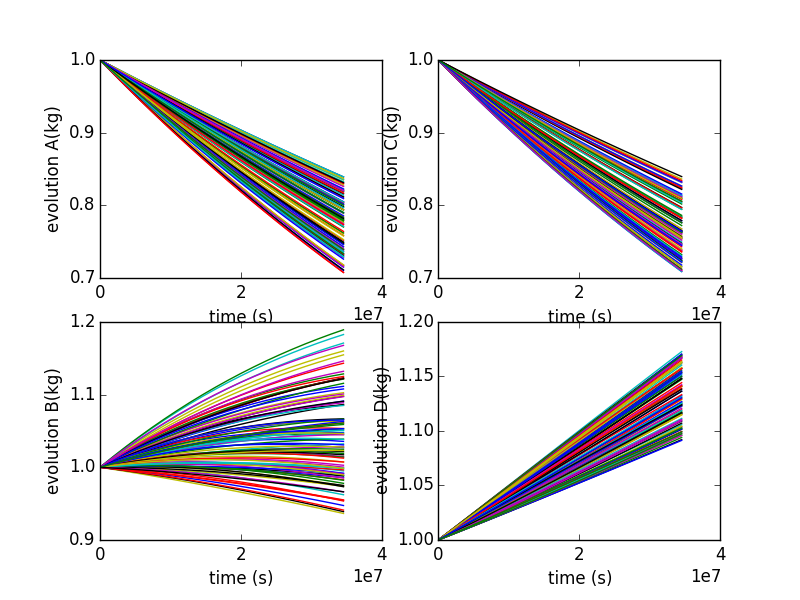
\includegraphics[scale=0.7]{pics/MC_histories.png}
  \caption{Plot of the histories generated by the MC sampling for variables $A,B,C,D$.}
  \label{fig:historiesMCPlotLine}
 \end{figure}
 %%%%%%%%%%%%%%%%%%%%%%%%%%%%%%%%%%%%%%%%%%%%%%%%%%%%%%%%%%
  In this block, both the Out-Stream types are constructed: 
  \begin{itemize}
    \item \textit{Print}: 
     \begin{itemize}
       \item named ``samples'' connected with the \textit{DataObjects} \textbf{Entity} ``samples'' 
                (\xmlNode{source})
       \item named ``histories'' connected with the \textit{DataObjects} \textbf{Entity} ``histories'' (\xmlNode{source})          
     \end{itemize}         
      When these objects get used, all the information contained in the 
      linked  \textit{DataObjects} are going 
    to be dumped in CSV files (\xmlNode{type}).
    \item \textit{Plot}: 
    \begin{itemize}
      \item named ``historiesPlot'' connected with the  \textit{DataObjects} 
      \textbf{Entity} ``samples''.  This plot will draw the final state of the
      variables $A,B,C,D$ with respect to the input variables $sigma$(s) 
      and $decay$(s) . 
      \item named ``samplesPlot3D'' connected with the  
      \textit{DataObjects} \textbf{Entity} ``histories''. This plot will draw the 
      evolution of the variables $A,B,C,D$;
    \end{itemize}
     Note that both plots are of type \textit{SubPlot}. Four plots
     are going to be placed in each of the figures.
  \end{itemize}   
   \item \textbf{\textit{Steps}}:   
\begin{lstlisting}[style=XML,morekeywords={arg,extension,pauseAtEnd,overwrite}]
  <Steps>
    <MultiRun name="sample">
      <Input 	    class="Files" 			 type="input">referenceInput.xml</Input>
      <Model 	    class="Models" 		 type="Code">testModel</Model>
      <Sampler 	class="Samplers" 		 type="MonteCarlo">monteCarlo</Sampler>
      <Output 	class="DataObjects"  type="PointSet">samples</Output>
      <Output 	class="DataObjects"  type="HistorySet">histories</Output>
    </MultiRun>
    <IOStep name="writeHistories" pauseAtEnd="True">
        <Input class="DataObjects" type="HistorySet">histories</Input>
        <Input class="DataObjects" type="PointSet">samples</Input>
        <Output 	class="OutStreamManager" type="Plot">samplesPlot3D</Output>
        <Output 	class="OutStreamManager" type="Plot">historyPlot</Output>
        <Output 	class="OutStreamManager" type="Print">samples</Output>
        <Output 	class="OutStreamManager" type="Print">histories</Output>
    </IOStep>
  </Steps>
\end{lstlisting}
 %%%%%%%%%%%%%%%%%%%%%%%%%%%%%%%%%%%%%%%%%%%%%%%%%%%%%%%%%%
 %figure samples
 \begin{figure}[h!]
  \centering
  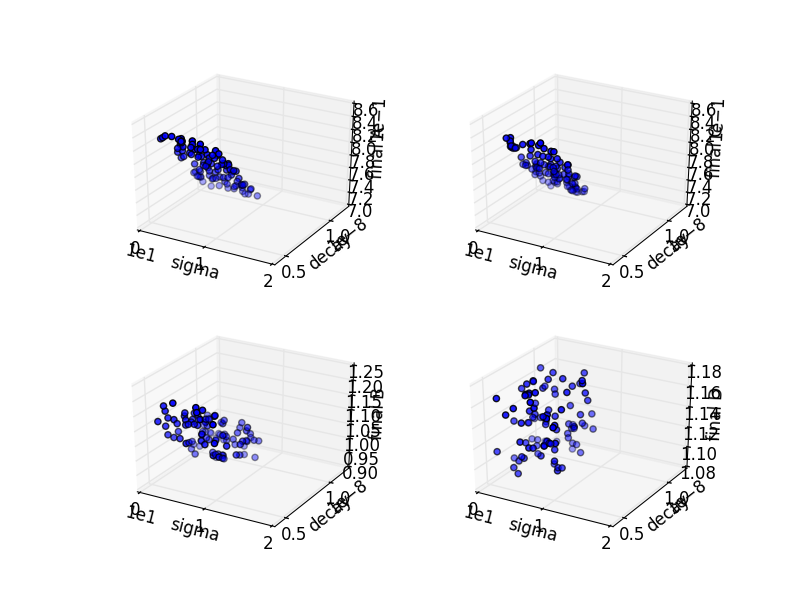
\includegraphics[scale=0.7]{pics/MC_pointsets.png}
  \caption{Plot of the samples generated by the MC sampling for variables $A,B,C,D$.}
  \label{fig:samplesMCPlotLine}
 \end{figure}
 %%%%%%%%%%%%%%%%%%%%%%%%%%%%%%%%%%%%%%%%%%%%%%%%%%%%%%%%%%
   Finally, all the previously defined \textbf{Entities} can be combined in 
   the \xmlNode{Steps} block. As inferable, 
   two \xmlNode{Steps} have been inputted:
   \begin{itemize}
     \item \xmlNode{MultiRun} named ``sample'', used to run the multiple  
     instances of the driven code and 
     collect the outputs in the two \textit{DataObjects}. As it can be
     seen, the \xmlNode{Sampler} is inputted to communicate to the 
     \textit{Step} that the driven code needs to
     be perturbed through the Monte-Carlo sampling;
     \item  \xmlNode{IOStep} named ``writeHistories'', used to 1) dump 
     the ``histories'' and ``samples'' \textit{DataObjects} 
     \textbf{Entity} in a CSV file and 2) plot the data in the PNG file and 
     on the screen.
   \end{itemize}
\end{enumerate} 
 Figures~\ref{fig:historiesMCPlotLine} and ~\ref{fig:samplesMCPlotLine}  report the evolution of the 
 variables $A,B,C,D$ and their final values, respectively.
%%%%%%%%%%%%%%%%%%%%%%%%%
%%%%%%%%          GRID          %%%%%%%% 
%%%%%%%%%%%%%%%%%%%%%%%%%
\subsection{Grid}
\label{sub:Grid}
The Grid sampling method (also known as Full Factorial Design of Experiment) represents one of the simplest methodologies that can be employed in order to explore the interaction of multiple random variables with respect
selected FOMs.
In this section, a brief theoretical 
background is reported. In addition,it is shown how to employ this methodology with RAVEN.
\subsubsection{Grid theory introduction}
\label{subsub:Gridtheory}
The goal of the Grid-based sampling strategy is to explore the interaction of multiple random 
variables (i.e. uncertainties) with respect to selected FOMs. Indeed, this method is mainly used to perform 
parametric analysis of the system response rather than a probabilistic one. This method discretizes the
domain of the uncertainties in a user-defined number of intervals (see Fig.~\ref{fig:GridDiscretization}) and 
record the response of the model (e.g. a system code) at each coordinate (i.e., combination of the uncertainties) of the grid.
\\ This method starts from the assumption that each coordinate on the grid is representative, with respect to the FOMs of interest, of the surrounding grid cell. In other words, it is assumed that the response of a system does not significantly change within the hyper-volume surrounding each grid coordinate (red square in Fig.~\ref{fig:GridDiscretization}).
 %%%%%%%%%%%%%%%%%%%%%%%%%%%%%%%%%%%%%%%%%%%%%%%%%%%%%%%%%%
 %figure history
 \begin{figure}[h!]
  \centering
  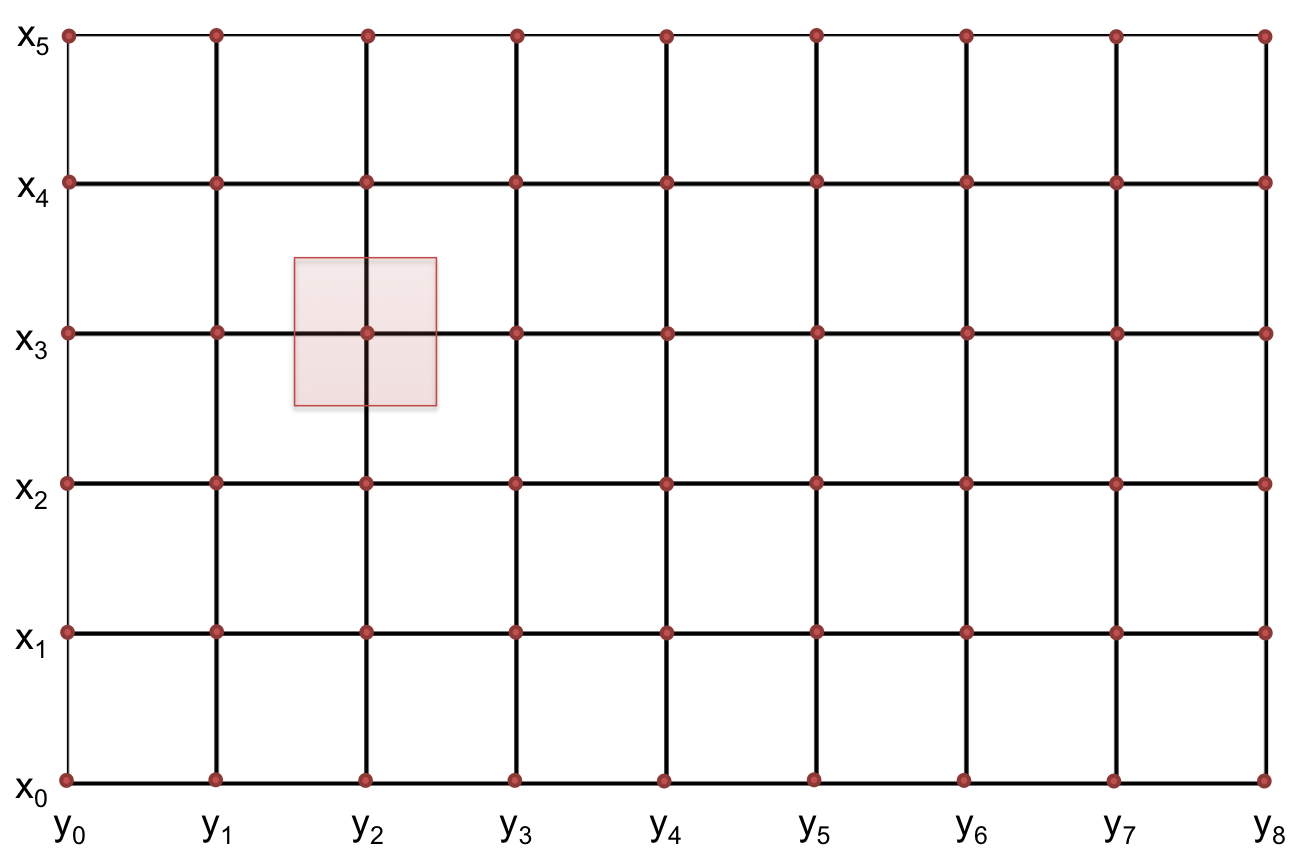
\includegraphics[scale=0.7]{pics/GridDiscretization.png}
  \caption{Example of 2-Dimensional grid discretization. }
  \label{fig:GridDiscretization}
 \end{figure}
 %%%%%%%%%%%%%%%%%%%%%%%%%%%%%%%%%%%%%%%%%%%%%%%%%%%%%%%%%%

Similarly to what has been already reported for the Monte-Carlo sampling, let's consider a random variable $X$ having PDF $pdf_{X}(x)$ and, consequentially, CDF $cdf_{X}(x)$ in the domain $\chi$. Then the expected value of a function $f$ of $X$ is as follows:
\begin{equation}
\begin{matrix}
\mathbb{E}(f(X)) =\sum_{x \in \chi} f(x)pdf_{X}(x) & if X \, discrete \\ 
\\ 
\mathbb{E}(f(X)) =\int_{x \in \chi} f(x)pdf_{X}(x) & \, if X \, \, continuous
\end{matrix}
\end{equation}
In the Grid approach, the domain of $X$ is discretized in a finite number of intervals. Recall that 
each node of this discretization is representative of the surrounding hyper-volume. This means that a weight 
needs to be associated with each coordinate of the resulting grid:
\begin{equation}
\begin{matrix}
  w_{i}= cdf_{X}(x_{i+1/2}) - cdf_{X}(x_{i-1/2})
\end{matrix}  
\end{equation}
Let's now consider 
a $n-$discretization of the domain of  $X$, $(x_{1},...,x_{n})$ and compute the mean of $f(x)$ over the discretization. Based on the previous equation, the computation of the expected value of $f(x)$ is as follows:
\begin{equation}
 \mathbb{E}(f(X)) \approx   \widetilde{f}_{n}(x) = \frac{1}{\sum_{i=1}^{n}w_{i}} \sum_{i=1}^{n} f(x_{i}) \times w_{i}
\end{equation}
If the number of uncertainties under consideration is greater than one ($m$), the above equation
becomes:
\begin{equation}
\mathbb{E}(f(\overline{X})) \approx   \widetilde{f}_{n}(\overline{x}) = \frac{1}{\sum_{i=1}^{n}\prod_{j=1}^{m}w_{i,j}} \sum_{i=1}^{n} f(\overline{x}_{i}) \times \prod_{j=1}^{m}w_{i,j}
\end{equation}

\subsubsection{Grid sampling through RAVEN}
\label{subsub:Gridexample}
The goal of this section is to show how to:
 \begin{enumerate}
   \item Set up a simple Grid sampling for performing a parametric analysis of a driven code;
   \item Load the outputs of the code into the RAVEN DataObjects system;
   \item Print out what contained in the DataObjects;
   \item Generate basic plots of the code result.
\end{enumerate}  
In order to accomplish these tasks, the following RAVEN \textbf{Entities} (XML blocks in the input files) are required:
\begin{enumerate}
   \item \textbf{\textit{RunInfo}}:
\begin{lstlisting}[style=XML,morekeywords={arg,extension,pauseAtEnd,overwrite}]
  <RunInfo>
    <JobName>ChapterVII-I/Grid</JobName>
    <Sequence>sample,writeHistories</Sequence>
    <WorkingDir>ChapterVII-I/Grid</WorkingDir>
    <batchSize>12</batchSize>
  </RunInfo>
\end{lstlisting}   
   As shown in Section~\ref{sub:EntitiesAndFlow}, the \textit{RunInfo} \textbf{Entity} is intended to set up the desired analysis.
   In this specific case, two steps (\xmlNode{Sequence}) are sequentially run 
   using 12 processors (\xmlNode{batchSize}). This means that
   12 instances of the driven code are  run simultaneously. 
   Every time a simulation ends, a new one is launched.
   \item \textbf{\textit{Files}}:
\begin{lstlisting}[style=XML,morekeywords={arg,extension,pauseAtEnd,overwrite}]
  <Files>
    <Input name="referenceInput.xml" type="input">referenceInput.xml</Input>
  </Files>
\end{lstlisting}
   Since the driven code uses a single input file, in this section the original input is placed. As described in the user manual~\cite{}
   the attribute  \xmlAttr{name} represents the alias that is used in all the other input blocks in order to refer to this file.
   \item \textbf{\textit{Models}}:
\begin{lstlisting}[style=XML,morekeywords={arg,extension,pauseAtEnd,overwrite}]
   <Models>
      <Code name="testModel" subType="GenericCode">
        <executable>
          ../physicalCode/analyticalbateman/AnalyticalDplMain.py
        </executable>
        <clargs arg="python" type="prepend"/>
        <clargs arg="" extension=".xml" type="input"/>
        <clargs arg="" extension=".csv" type="output"/>
        <prepend>python</prepend>
      </Code>
    <Models>
\end{lstlisting}
 The Model here is represented by the 
 \textbf{AnalyticalBateman}, which already dumps its output file in a 
 CSV format (standard format that RAVEN can read). For this reason,
 the \textit{GenericCode} interface is used.
   \item \textbf{\textit{Distributions}}:
\begin{lstlisting}[style=XML,morekeywords={arg,extension,pauseAtEnd,overwrite}]
  <Distributions>
      <Uniform name="sigma">
          <lowerBound>1</lowerBound>
          <upperBound>10</upperBound>
      </Uniform>
      <Uniform name="decayConstant">
          <lowerBound>0.000000005</lowerBound>
          <upperBound>0.000000010</upperBound>
      </Uniform>
  </Distributions>   
\end{lstlisting}
  In the Distributions XML section, the stochastic model for the 
  uncertainties  treated by the Grid sampling are reported. In 
  this case two distributions are defined: 
  \begin{itemize}
    \item $sigma \sim \mathbb{U}(1,10)$, used to model the uncertainties 
    associated with  the Model \textit{sigma}(s);
    \item  $decayConstant \sim \mathbb{U}(0.5e-8,1e-8)$,  used to 
    model the uncertainties 
    associated with  the Model \textit{decay constants}.
  \end{itemize}
   \item \textbf{\textit{Samplers}}:
\begin{lstlisting}[style=XML,morekeywords={arg,extension,pauseAtEnd,overwrite}]
  <Samplers>
    <Grid name="grid">
      <variable name="sigma-A">
        <distribution>sigma</distribution>
        <grid construction="equal" steps="1" type="value">2 4.0</grid>
      </variable>
      <variable name="decay-A">
        <distribution>decayConstant</distribution>
        <grid construction="custom" type="value">0.000000005  0.000000008</grid>
      </variable>
      <variable name="sigma-B">
          <distribution>sigma</distribution>
          <grid construction="equal" steps="1" type="CDF">0.1 0.8</grid>
      </variable>
      <variable name="decay-B">
          <distribution>decayConstant</distribution>
          <grid construction="equal" steps="1" type="CDF">0.1 0.8</grid>
      </variable>
      <variable name="sigma-C">
          <distribution>sigma</distribution>
          <grid construction="equal" steps="1" type="value">4 5</grid>
      </variable>
      <variable name="decay-C">
          <distribution>decayConstant</distribution>
          <grid construction="equal" steps="1" type="CDF">0.1 0.5</grid>
      </variable>
      <variable name="sigma-D">
          <distribution>sigma</distribution>
          <grid construction="equal" steps="1" type="CDF">0.4 0.8</grid>
      </variable>
      <variable name="decay-D">
          <distribution>decayConstant</distribution>
          <grid construction="equal" steps="1" type="CDF">0.1 0.8</grid>
      </variable>
    </Grid>
  </Samplers>  
\end{lstlisting}
  In order to employ the Grid sampling strategy, a 
  \xmlNode{Grid} node needs to be specified. As shown above, in each variable section, the  \xmlNode{grid} is defined. 
  The number of samples finally requested are equal to $n_{samples} = \prod_{i=1}^{n} n_{steps_{i}+1} = 256$.
  Note that, for each variable, can be defined either in probability (CDF) or in absolute value.  
   \item \textbf{\textit{DataObjects}}:
\begin{lstlisting}[style=XML,morekeywords={arg,extension,pauseAtEnd,overwrite}]
  <DataObjects>
    <PointSet name="samples">
      <Input>
        sigma-A,sigma-B,sigma-C,sigma-D,
        decay-A,decay-B,decay-C,decay-D
      </Input>
      <Output>A,B,C,D,time</Output>
    </PointSet>
    <HistorySet name="histories">
        <Input>
          sigma-A,sigma-B,sigma-C,sigma-D,
          decay-A,decay-B,decay-C,decay-D
        </Input>
        <Output>A,B,C,D,time</Output>
    </HistorySet>
  </DataObjects>
\end{lstlisting}
  Int this block, two \textit{DataObjects} are defined: 1) PointSet named 
  ``samples'', and 2) HistorySet named ``histories''.
  In the \xmlNode{Input} node all the variables 
  perturbed through the Grid strategy are listed. In this way, any
  realization in the input space is linked to the outputs listed in  the 
  \xmlNode{Output} node.
   \item \textbf{\textit{OutStreamManager}}:   
\begin{lstlisting}[style=XML,morekeywords={arg,extension,pauseAtEnd,overwrite}]
  <OutStreamManager>
    <Print name="samples">
      <type>csv</type>
      <source>samples</source>
    </Print>
    <Print name="histories">
      <type>csv</type>
      <source>histories</source>
    </Print>
    <Plot dim="2" name="historiesPlot" overwrite="false" verbosity="debug">
        <plotSettings>
            <gridSpace>2 2</gridSpace>
            <plot>
                <type>line</type>
                <x>histories|Output|time</x>
                <y>histories|Output|A</y>
                <color>blue</color>
                <gridLocation>
                  <x>0</x>
                  <y>0</y>
                </gridLocation>
                <xlabel>time (s)</xlabel>
                <ylabel>evolution A(kg)</ylabel>
            </plot>
            <plot>
                <type>line</type>
                <x>histories|Output|time</x>
                <y>histories|Output|B</y>
                <color>red</color>
                <gridLocation>
                    <x>1</x>
                    <y>0</y>
                </gridLocation>
                <xlabel>time (s)</xlabel>
                <ylabel>evolution B(kg)</ylabel>
            </plot>
            <plot>
                <type>line</type>
                <x>histories|Output|time</x>
                <y>histories|Output|C</y>
                <color>yellow</color>
                <gridLocation>
                    <x>0</x>
                    <y>1</y>
                </gridLocation>
                <xlabel>time (s)</xlabel>
                <ylabel>evolution C(kg)</ylabel>
            </plot>
            <plot>
                <type>line</type>
                <x>histories|Output|time</x>
                <y>histories|Output|D</y>
                <color>black</color>
                <gridLocation>
                    <x>1</x>
                    <y>1</y>
                </gridLocation>
                <xlabel>time (s)</xlabel>
                <ylabel>evolution D(kg)</ylabel>
            </plot>
        </plotSettings>
        <actions>
            <how>png,screen</how>
            <title>
                <text> </text>
            </title>
        </actions>
    </Plot>
    <Plot dim="3" name="samplesPlot3D" overwrite="false" verbosity="debug">
        <plotSettings>
            <gridSpace>2 2</gridSpace>
            <plot>
                <type>scatter</type>
                <x>samples|Input|sigma-A</x>
                <y>samples|Input|decay-A</y>
                <z>samples|Output|A</z>
                <color>blue</color>
                <gridLocation>
                  <x>0</x>
                  <y>0</y>
                </gridLocation>
                <xlabel>sigma</xlabel>
                <ylabel>decay</ylabel>
                <zlabel>final A</zlabel>
            </plot>
            <plot>
                <type>scatter</type>
                <x>samples|Input|sigma-B</x>
                <y>samples|Input|decay-B</y>
                <z>samples|Output|B</z>
                <color>red</color>
                <gridLocation>
                    <x>1</x>
                    <y>0</y>
                </gridLocation>
                <xlabel>sigma</xlabel>
                <ylabel>decay</ylabel>
                <zlabel>final B</zlabel>
            </plot>
            <plot>
                <type>scatter</type>
                <type>scatter</type>
                <x>samples|Input|sigma-C</x>
                <y>samples|Input|decay-C</y>
                <z>samples|Output|C</z>
                <color>yellow</color>
                <gridLocation>
                    <x>0</x>
                    <y>1</y>
                </gridLocation>
                <xlabel>sigma</xlabel>
                <ylabel>decay</ylabel>
                <zlabel>final C</zlabel>
            </plot>
            <plot>
                <type>scatter</type>
                <x>samples|Input|sigma-D</x>
                <y>samples|Input|decay-D</y>
                <z>samples|Output|D</z>
                <color>black</color>
                <gridLocation>
                    <x>1</x>
                    <y>1</y>
                </gridLocation>
                <xlabel>sigma</xlabel>
                <ylabel>decay</ylabel>
                <zlabel>final D</zlabel>
            </plot>
            <xlabel>sigma</xlabel>
            <ylabel>decay</ylabel>
            <zlabel>final response</zlabel>
        </plotSettings>
        <actions>
            <how>png,screen</how>
            <title>
                <text> </text>
            </title>
        </actions>
    </Plot>
  </OutStreamManager>
\end{lstlisting}
 %%%%%%%%%%%%%%%%%%%%%%%%%%%%%%%%%%%%%%%%%%%%%%%%%%%%%%%%%%
 %figure histories
 \begin{figure}[h!]
  \centering
  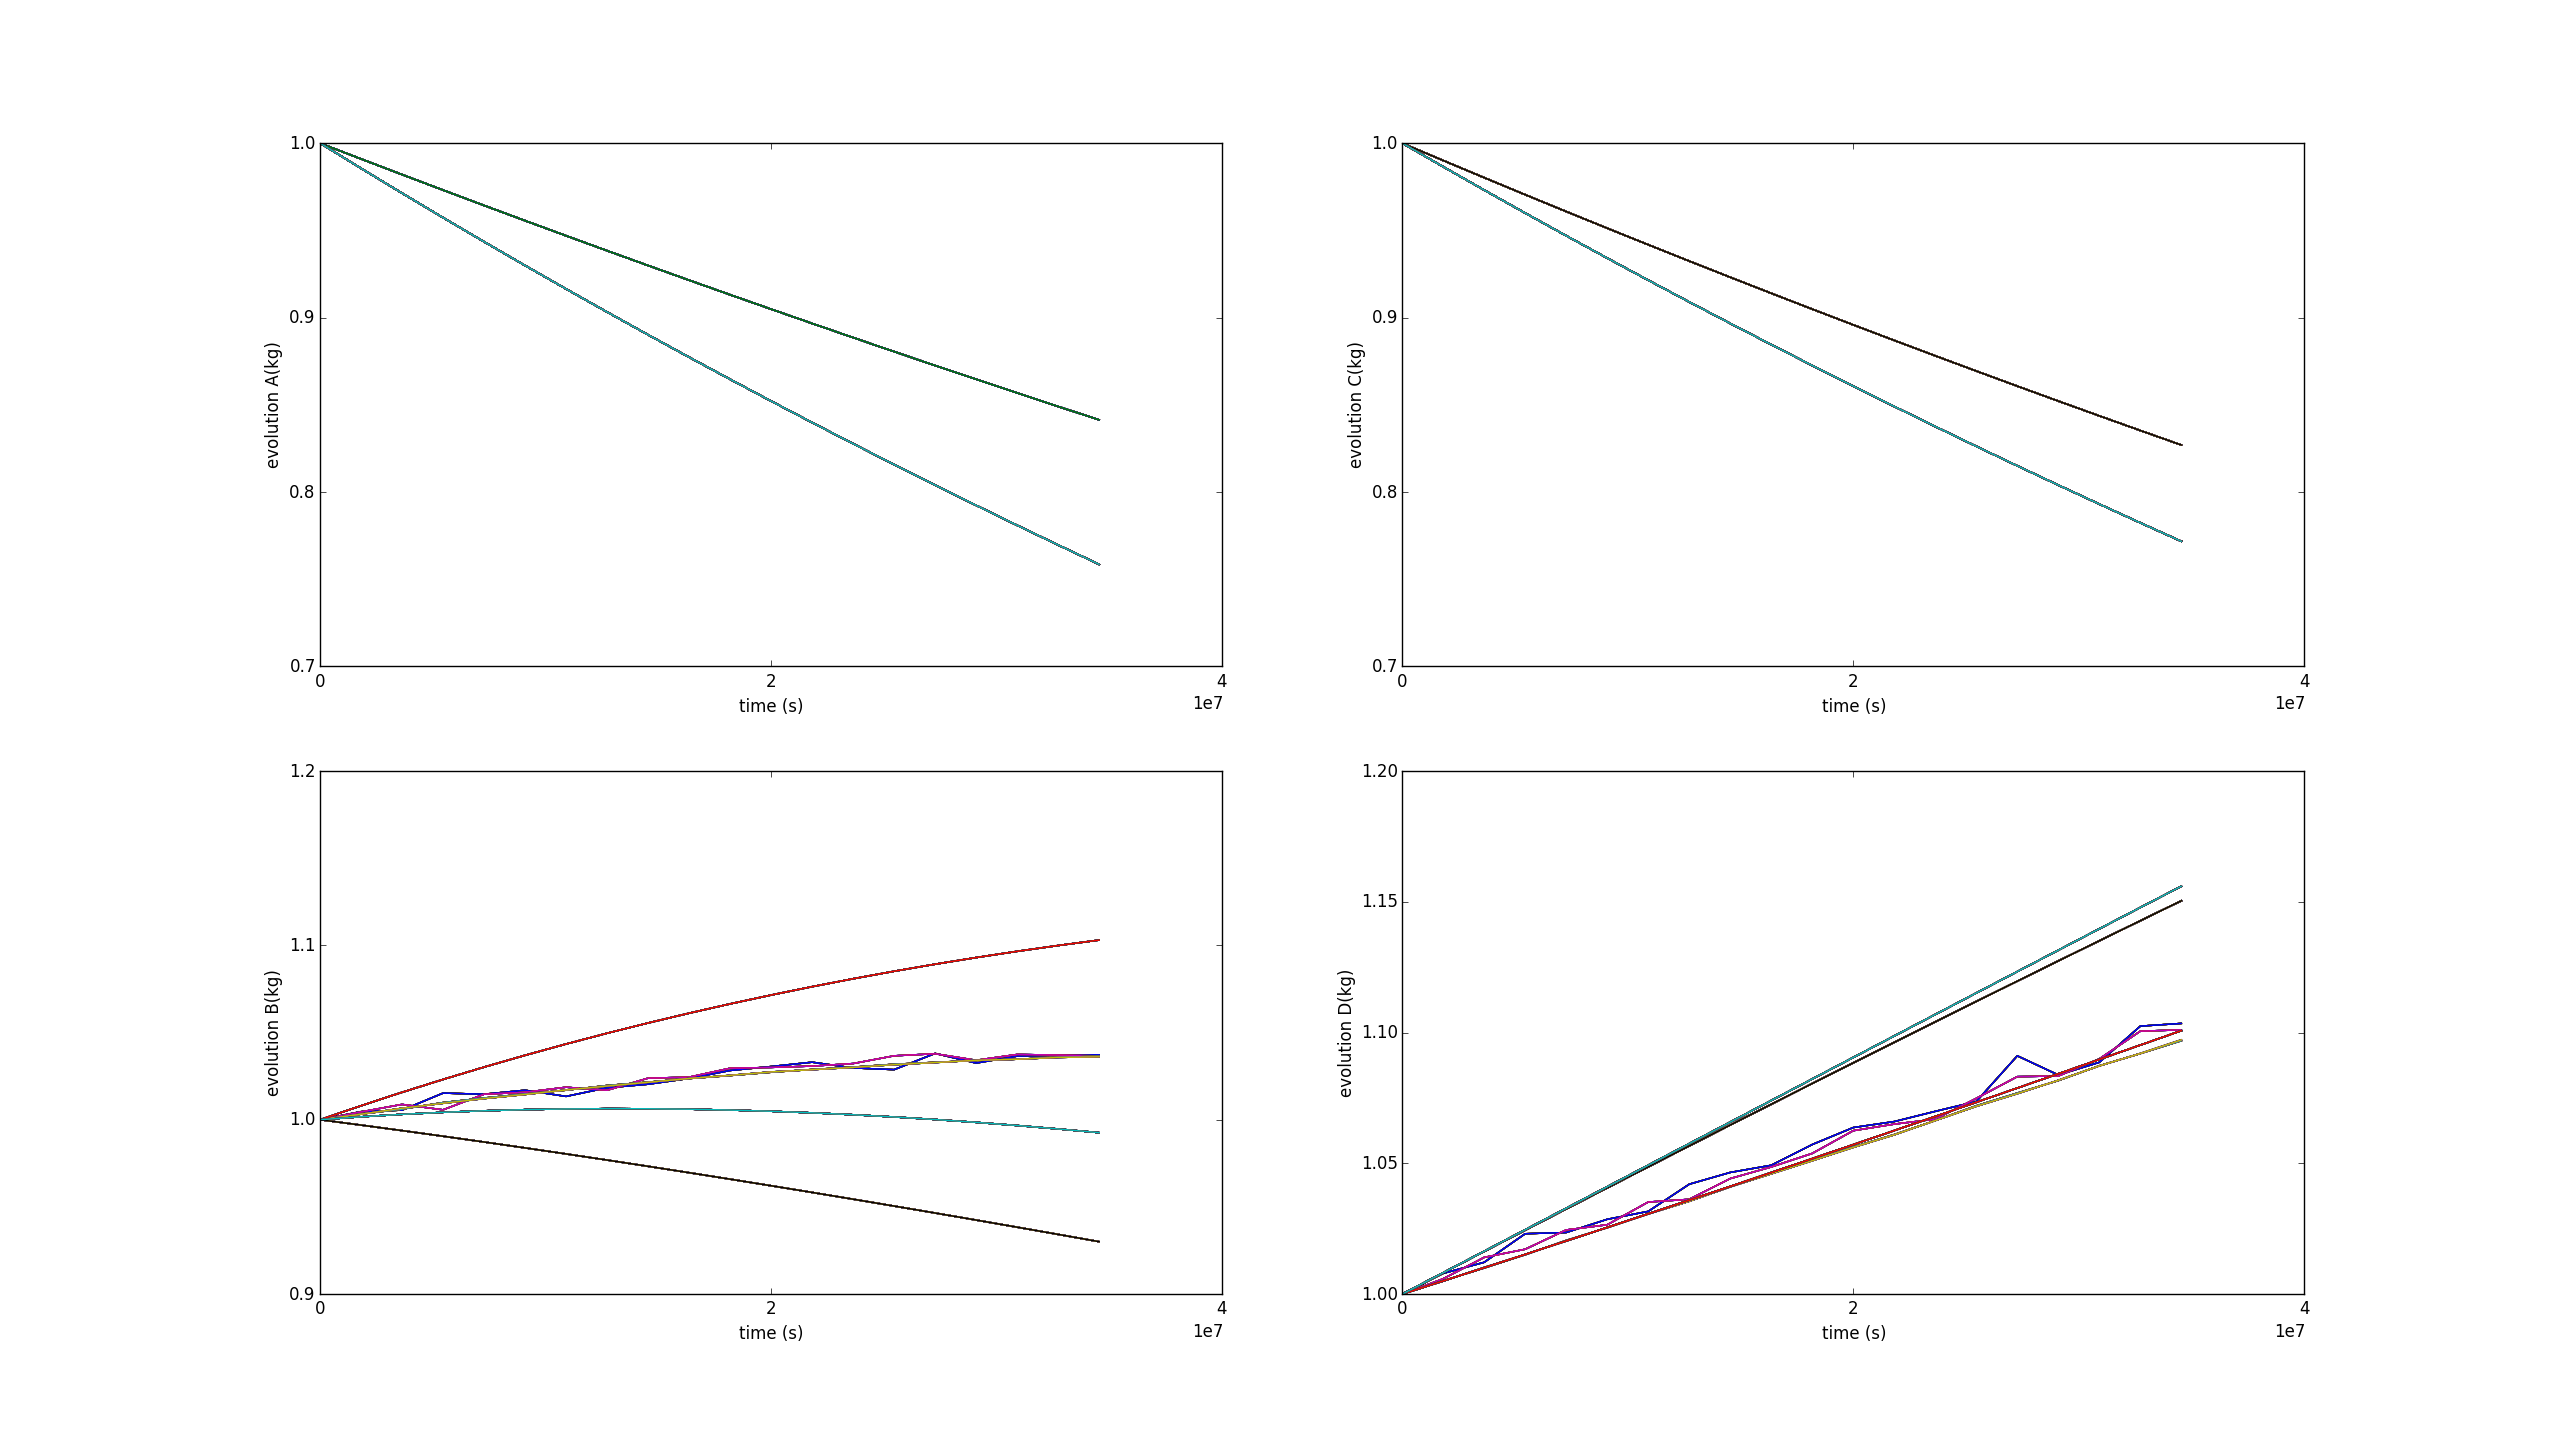
\includegraphics[scale=0.7]{pics/Grid_histories.png}
  \caption{Plot of the histories generated by the Grid sampling for variables $A,B,C,D$.}
  \label{fig:historiesGridPlotLine}
 \end{figure}
 %%%%%%%%%%%%%%%%%%%%%%%%%%%%%%%%%%%%%%%%%%%%%%%%%%%%%%%%%%
  In this block, both the Out-Stream types are constructed: 
  \begin{itemize}
    \item \textit{Print}: 
     \begin{itemize}
       \item named ``samples'' connected with the \textit{DataObjects} \textbf{Entity} ``samples'' 
                (\xmlNode{source})
       \item named ``histories'' connected with the \textit{DataObjects} \textbf{Entity} ``histories'' (\xmlNode{source})          
     \end{itemize}         
      When these objects get used, all the information contained in the 
      linked  \textit{DataObjects} are going 
    to be dumped in CSV files (\xmlNode{type}).
    \item \textit{Plot}: 
    \begin{itemize}
      \item named ``historiesPlot'' connected with the  \textit{DataObjects} 
      \textbf{Entity} ``samples''.  This plot will draw the final state of the
      variables $A,B,C,D$ with respect to the input variables $sigma$(s) 
      and $decay$(s) . 
      \item named ``samplesPlot3D'' connected with the  
      \textit{DataObjects} \textbf{Entity} ``histories''. This plot will draw the 
      evolution of the variables $A,B,C,D$;
    \end{itemize}
     As it can be noticed, both plots are of type \textit{SubPlot}. Four plots
     are placed in each of the figures.
  \end{itemize}   
   \item \textbf{\textit{Steps}}:   
\begin{lstlisting}[style=XML,morekeywords={arg,extension,pauseAtEnd,overwrite}]
  <Steps>
    <MultiRun name="sample">
      <Input 	    class="Files" 			 type="input">referenceInput.xml</Input>
      <Model 	    class="Models" 		 type="Code">testModel</Model>
      <Sampler 	class="Samplers" 		 type="Grid">grid</Sampler>
      <Output 	class="DataObjects"  type="PointSet">samples</Output>
      <Output 	class="DataObjects"  type="HistorySet">histories</Output>
    </MultiRun>
    <IOStep name="writeHistories" pauseAtEnd="True">
        <Input class="DataObjects" type="HistorySet">histories</Input>
        <Input class="DataObjects" type="PointSet">samples</Input>
        <Output 	class="OutStreamManager" type="Plot">samplesPlot3D</Output>
        <Output 	class="OutStreamManager" type="Plot">historyPlot</Output>
        <Output 	class="OutStreamManager" type="Print">samples</Output>
        <Output 	class="OutStreamManager" type="Print">histories</Output>
    </IOStep>
  </Steps>
\end{lstlisting}
 %%%%%%%%%%%%%%%%%%%%%%%%%%%%%%%%%%%%%%%%%%%%%%%%%%%%%%%%%%
 %figure samples
 \begin{figure}[h!]
  \centering
  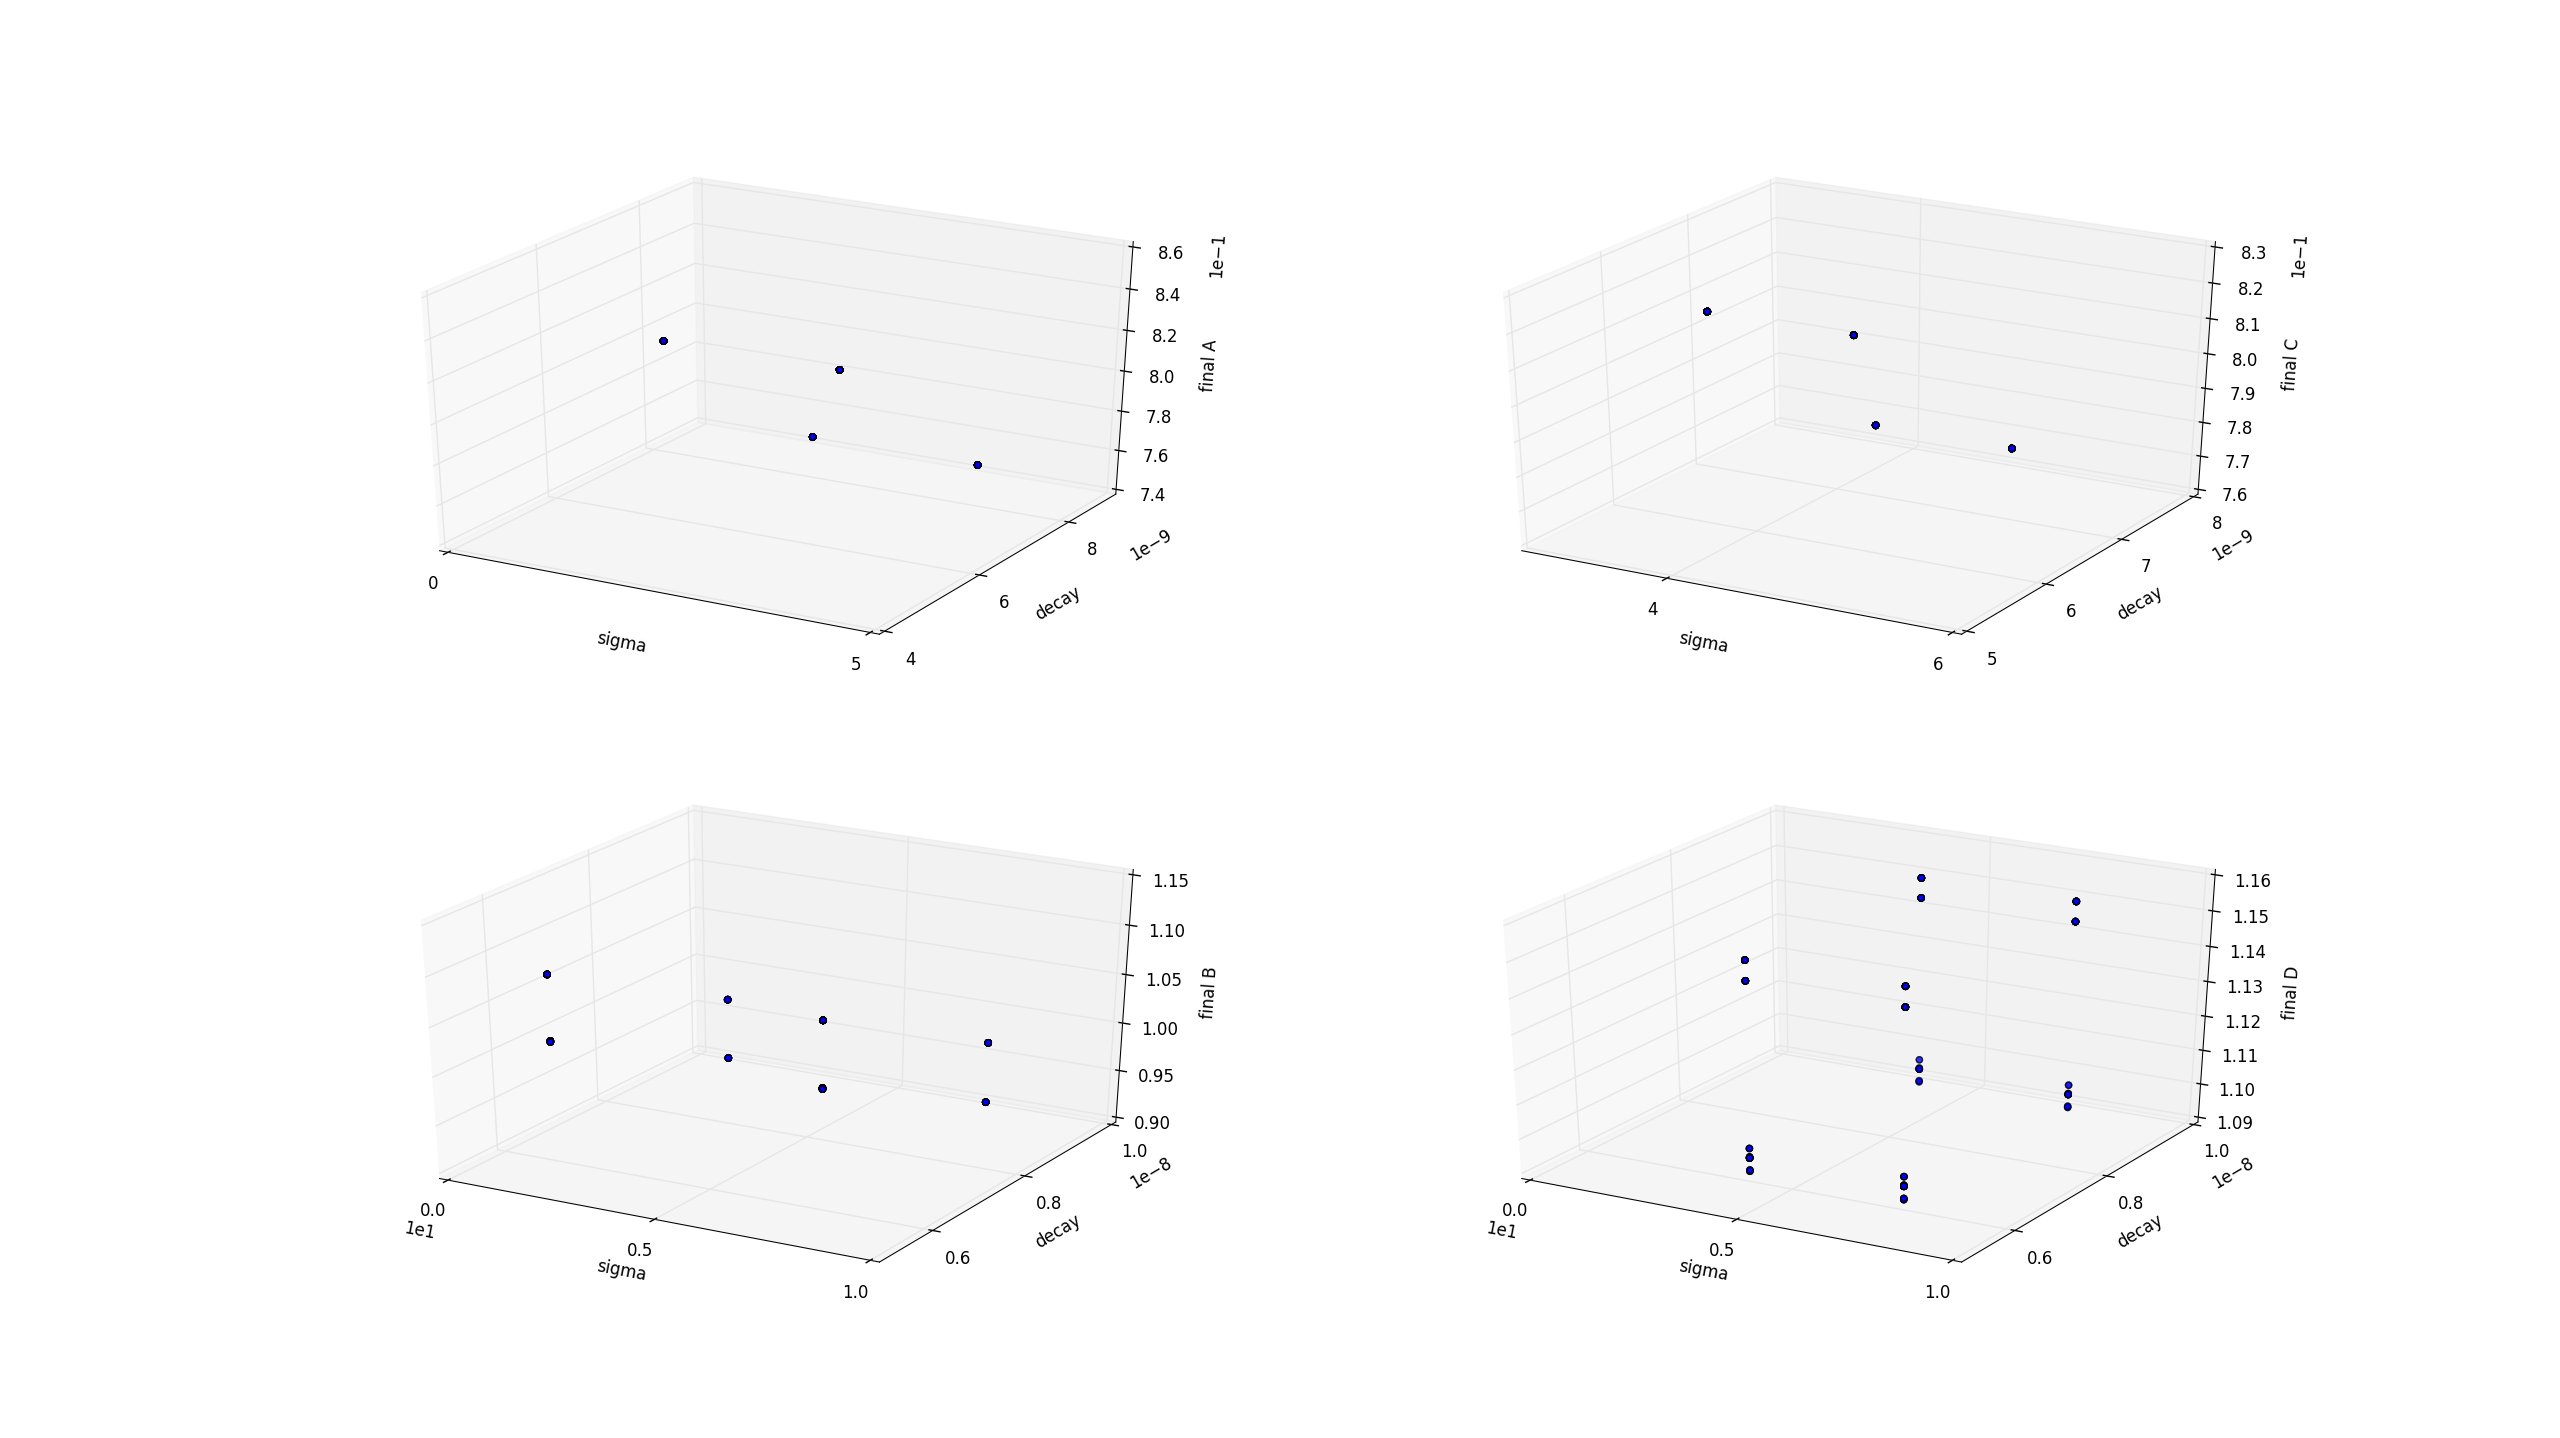
\includegraphics[scale=0.7]{pics/Grid_pointsets.png}
  \caption{Plot of the samples generated by the Grid sampling for variables $A,B,C,D$.}
  \label{fig:samplesGridPlotLine}
 \end{figure}
 %%%%%%%%%%%%%%%%%%%%%%%%%%%%%%%%%%%%%%%%%%%%%%%%%%%%%%%%%%
   Finally, all the previously defined \textbf{Entities} can be combined in 
   the \xmlNode{Steps} block. As inferable, 
   two \xmlNode{Steps} have been inputted:
   \begin{itemize}
     \item \xmlNode{MultiRun} named ``sample'', is used to run the multiple  
     instances of the code and 
     collect the outputs in the two \textit{DataObjects}. As it can be
     seen, the \xmlNode{Sampler} is inputted to communicate to the 
     \textit{Step} that the driven code needs to
     be perturbed through the Grid sampling;
     \item  \xmlNode{IOStep} named ``writeHistories'', used to 1) dump 
     the ``histories'' and ``samples'' \textit{DataObjects} 
     \textbf{Entity} in a CSV file and 2) plot the data in the PNG file and 
     on the screen.
   \end{itemize}
\end{enumerate} 
 As previously mentioned, Figures~\ref{fig:historiesGridPlotLine} and ~\ref{fig:samplesGridPlotLine}  report the evolution of the 
 variables $A,B,C,D$ and their final values, respectively.

%%%%%%%%%%%%%%%%%%%%%%%%%
%%%%%%%%    STRATIFIED    %%%%%%%% 
%%%%%%%%%%%%%%%%%%%%%%%%%
\subsection{Stratified}
\label{sub:Stratified}
The Stratified sampling is a class of methods that relies on the assumption that the input space (i.e. uncertainties) 
can be separated in regions (strata) based on similarity of the response of the system for input set within the
same strata. Following this assumption, the most rewarding (in terms of computational cost vs. knowledge gain) 
sampling strategy would be to place one sample for each region. In this way, the same information is not 
collected more than once and all the prototypical behavior are sampled at least once. In 
Fig.~\ref{fig:StratifiedSamplingExample}, the Stratified sampling approach is exemplified. 
 \begin{figure}[h!]
  \centering
  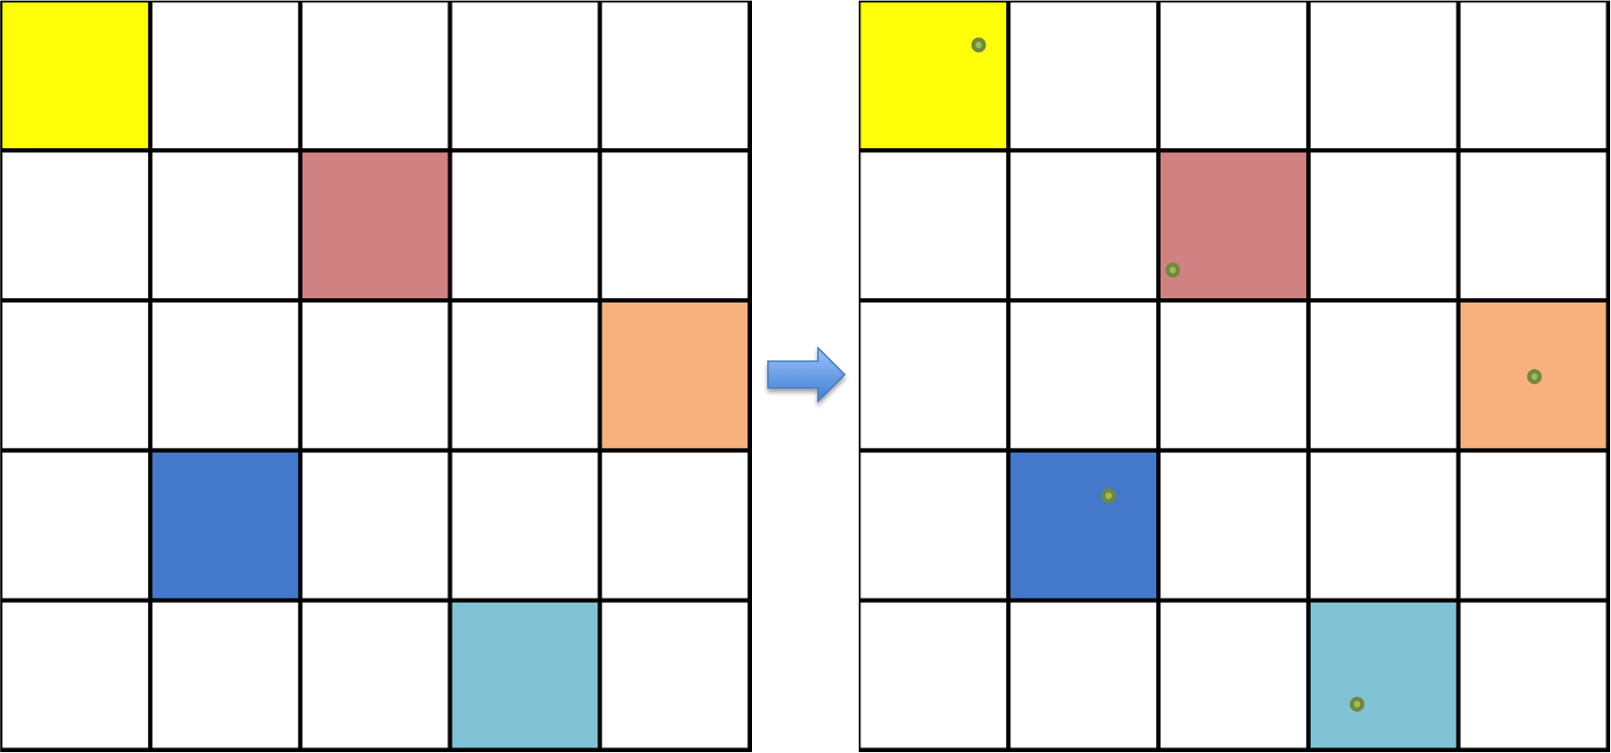
\includegraphics[scale=0.55]{pics/StratifiedSamplingExample.png}
  \caption{Example of Stratified sampling approach.}
  \label{fig:StratifiedSamplingExample}
 \end{figure}
\\In this section, a brief theoretical 
background is reported. In addition,it is shown how to employ this methodology with RAVEN.
\subsubsection{Stratified theory introduction}
\label{subsub:Stratifiedtheory}
The Stratified sampling approach is a method for the exploration of the input space that consists of dividing the uncertain domain into subgroups before sampling. In the Stratified sampling, these subgroups must be:
\begin{itemize}
  \item mutually exclusive: every element in the population must be assigned to only one stratum (subgroup)
  \item collectively exhaustive: no population element can be excluded
\end{itemize}
Then, simple random sampling or systematic sampling is applied within each stratum. The Latin Hyper-Cube sampling represents a specialized version of the stratified approach, when the domain strata are constructed in equally-probable CDF bins.
\\Similarly to what has been already reported for the Grid sampling, let's consider a set of  $m$ random variables $X_{j}, \, j=1,..,m$ having PDFs $pdf_{X_{j}}(x_{j})$ and, consequentially, CDF $cdf_{X_{j}}(x_{j})$ in the domain $\chi_{j}$. Then the expected value of a function $f$ of $X_{j}, \, j=1,..,m$ is as follows:
\begin{equation}
\begin{matrix}
\mathbb{E}(f(\overline{X})) =\sum f(x)   \prod_{j=1}^{m} pdf_{X_{j}}(x_{j}) & if \overline{X} \, discrete \\ 
\\ 
\mathbb{E}(f(\overline{X})) =\int f(x)\prod_{j=1}^{m} pdf_{X_{j}}(x_{j}) & \, if \overline{X} \, \, continuous
\end{matrix}
\end{equation}
In the Stratified approach, the domain of $\overline{X}$ is discretized in a set of strata. Consequentially, similarly to the Grid sampling, a weight needs to be associated with each realization in the input space:
\begin{equation}
\begin{matrix}
  w_{i}= \frac{\prod_{j=1}^{m} \left [  cdf_{X_{j}}(x_{i,j+1}) - cdf_{X_{j}}(x_{i,j}) \right ]}{\sum_{points}\prod_{j=1}^{m} \left [  cdf_{X_{j}}(x_{i,j+1}) - cdf_{X_{j}}(x_{i,j}) \right ]}
\end{matrix}  
\end{equation}
Each realization carries a weight representative of each stratum.
\\Let's now consider 
to take a $n-$strata of the domain of  $\overline{X}$, and compute the expected value of $f(x)$ over the discretization. Based on the previous equation, the computation of the expected value of $f(x)$ is as follows:
\begin{equation}
 \mathbb{E}(f(\overline{X})) \approx   \widetilde{f}_{n}(\overline{x}) = \frac{1}{\sum_{i=1}^{n}w_{i}} \sum_{i=1}^{n} f(\overline{x}_{i}) \times w_{i}
\end{equation}
\subsubsection{Stratified sampling through RAVEN}
\label{subsub:Stratifiedexample}
The goal of this section is to show how to:
 \begin{enumerate}
   \item Set up a simple Stratified sampling in order to perform a parametric analysis on a driven code
   \item Load the outputs of the code into the RAVEN DataObjects system
   \item Print out what contained in the DataObjects
   \item Generate basic plots of the code result
\end{enumerate}  
In order to accomplish these tasks, the following RAVEN \textbf{Entities} (XML blocks in the input files) are defined:
\begin{enumerate}
   \item \textbf{\textit{RunInfo}}:
\begin{lstlisting}[style=XML,morekeywords={arg,extension,pauseAtEnd,overwrite}]
  <RunInfo>
    <JobName>ChapterVII-I/Stratified</JobName>
    <Sequence>sample,writeHistories</Sequence>
    <WorkingDir>ChapterVII-I/Stratified</WorkingDir>
    <batchSize>12</batchSize>
  </RunInfo>
\end{lstlisting}   
   As reported in Section~\ref{sub:EntitiesAndFlow}, the \textit{RunInfo} \textbf{Entity} is intended to set up the analysis 
   that the user wants to perform. In this specific case, two steps (\xmlNode{Sequence}) are  run 
   using 12 processors (\xmlNode{batchSize}). This means that
   12 instances of the driven code are run simultaneously. 
   Every time a simulation ends, a new one is launched.
   \item \textbf{\textit{Files}}:
\begin{lstlisting}[style=XML,morekeywords={arg,extension,pauseAtEnd,overwrite}]
  <Files>
    <Input name="referenceInput.xml" type="input">referenceInput.xml</Input>
  </Files>
\end{lstlisting}
   Since the considered code uses a single input file, in this section the original input is placed. 
   The attribute  \xmlAttr{name} represents the alias that is going to be used in all the other input blocks in order to refer to this file.
   \item \textbf{\textit{Models}}:
\begin{lstlisting}[style=XML,morekeywords={arg,extension,pauseAtEnd,overwrite}]
   <Models>
      <Code name="testModel" subType="GenericCode">
        <executable>
          ../physicalCode/analyticalbateman/AnalyticalDplMain.py
        </executable>
        <clargs arg="python" type="prepend"/>
        <clargs arg="" extension=".xml" type="input"/>
        <clargs arg="" extension=".csv" type="output"/>
        <prepend>python</prepend>
      </Code>
    <Models>
\end{lstlisting}
 The Model here is represented by the 
 \textbf{AnalyticalBateman}, which already dumps its output file in a 
 CSV format (standard format that RAVEN can read). For this reason,
 the \textit{GenericCode} interface is used.
   \item \textbf{\textit{Distributions}}:
\begin{lstlisting}[style=XML,morekeywords={arg,extension,pauseAtEnd,overwrite}]
  <Distributions>
      <Uniform name="sigma">
          <lowerBound>1</lowerBound>
          <upperBound>10</upperBound>
      </Uniform>
      <Uniform name="decayConstant">
          <lowerBound>0.000000005</lowerBound>
          <upperBound>0.000000010</upperBound>
      </Uniform>
  </Distributions>   
\end{lstlisting}
  In the Distributions XML section, the stochastic model for the 
  uncertainties  treated by the Stratified sampling are reported. In 
  this case two distributions are defined: 
  \begin{itemize}
    \item $sigma \sim \mathbb{U}(1,10)$, used to model the uncertainties 
    associated with  the Model \textit{sigma}(s);
    \item  $decayConstant \sim \mathbb{U}(0.5e-8,1e-8)$,  used to 
    model the uncertainties 
    associated with  the Model \textit{decay constants}.
  \end{itemize}
   \item \textbf{\textit{Samplers}}:
\begin{lstlisting}[style=XML,morekeywords={arg,extension,pauseAtEnd,overwrite}]
    <Stratified name="stratified">
      <variable name="sigma-A">
        <distribution>sigma</distribution>
        <grid construction="equal" steps="100" type="value">2 4.0</grid>
      </variable>
      <variable name="decay-A">
        <distribution>decayConstant</distribution>
        <grid construction="equal" steps="100" type="value">0.000000005 0.000000008</grid>
      </variable>
      <variable name="sigma-B">
          <distribution>sigma</distribution>
          <grid construction="equal" steps="100" type="CDF">0.1 0.8</grid>
      </variable>
      <variable name="decay-B">
          <distribution>decayConstant</distribution>
          <grid construction="equal" steps="100" type="CDF">0.1 0.8</grid>
      </variable>
      <variable name="sigma-C">
          <distribution>sigma</distribution>
          <grid construction="equal" steps="100" type="value">1.0 5</grid>
      </variable>
      <variable name="decay-C">
          <distribution>decayConstant</distribution>
          <grid construction="equal" steps="100" type="CDF">0.1 0.5</grid>
      </variable>
      <variable name="sigma-D">
          <distribution>sigma</distribution>
          <grid construction="equal" steps="100" type="CDF">0.4 0.8</grid>
      </variable>
      <variable name="decay-D">
          <distribution>decayConstant</distribution>
          <grid construction="equal" steps="100" type="CDF">0.1 0.8</grid>
      </variable>
    </Stratified> 
\end{lstlisting}
  In order to employ the Stratified sampling strategy, a 
  \xmlNode{Stratified} node needs to be specified. In each variable section, the  \xmlNode{grid} is defined. 
  It is important to mention that the number of \xmlAttr{steps} needs to be the same for each of the variables,
  since, as reported in previous section, the Stratified sampling strategy it discretizes the domain in strata. 
  The number of samples finally requested is equal to $n_{samples} = n_{steps} = 100$.
  If the grid for each variables is defined in CDF and of  \xmlAttr{type} = ``equal'', the Stratified
  sampling corresponds to the well-known Latin Hyper Cube sampling.
   \item \textbf{\textit{DataObjects}}:
\begin{lstlisting}[style=XML,morekeywords={arg,extension,pauseAtEnd,overwrite}]
  <DataObjects>
    <PointSet name="samples">
      <Input>
        sigma-A,sigma-B,sigma-C,sigma-D,
        decay-A,decay-B,decay-C,decay-D
      </Input>
      <Output>A,B,C,D,time</Output>
    </PointSet>
    <HistorySet name="histories">
        <Input>
          sigma-A,sigma-B,sigma-C,sigma-D,
          decay-A,decay-B,decay-C,decay-D
        </Input>
        <Output>A,B,C,D,time</Output>
    </HistorySet>
  </DataObjects>
\end{lstlisting}
  In this block, two \textit{DataObjects} are defined: 1) PointSet named 
  ``samples'', 2) HistorySet named ``histories''.
  In the \xmlNode{Input} node all the variables 
  perturbed through the Stratified strategy are listed. In this way, any
  realization in the input space is linked to the outputs listed in  the 
  \xmlNode{Output} node.
   \item \textbf{\textit{OutStreamManager}}:   
\begin{lstlisting}[style=XML,morekeywords={arg,extension,pauseAtEnd,overwrite}]
  <OutStreamManager>
    <Print name="samples">
      <type>csv</type>
      <source>samples</source>
    </Print>
    <Print name="histories">
      <type>csv</type>
      <source>histories</source>
    </Print>
    <Plot dim="2" name="historiesPlot" overwrite="false" verbosity="debug">
        <plotSettings>
            <gridSpace>2 2</gridSpace>
            <plot>
                <type>line</type>
                <x>histories|Output|time</x>
                <y>histories|Output|A</y>
                <color>blue</color>
                <gridLocation>
                  <x>0</x>
                  <y>0</y>
                </gridLocation>
                <xlabel>time (s)</xlabel>
                <ylabel>evolution A(kg)</ylabel>
            </plot>
            <plot>
                <type>line</type>
                <x>histories|Output|time</x>
                <y>histories|Output|B</y>
                <color>red</color>
                <gridLocation>
                    <x>1</x>
                    <y>0</y>
                </gridLocation>
                <xlabel>time (s)</xlabel>
                <ylabel>evolution B(kg)</ylabel>
            </plot>
            <plot>
                <type>line</type>
                <x>histories|Output|time</x>
                <y>histories|Output|C</y>
                <color>yellow</color>
                <gridLocation>
                    <x>0</x>
                    <y>1</y>
                </gridLocation>
                <xlabel>time (s)</xlabel>
                <ylabel>evolution C(kg)</ylabel>
            </plot>
            <plot>
                <type>line</type>
                <x>histories|Output|time</x>
                <y>histories|Output|D</y>
                <color>black</color>
                <gridLocation>
                    <x>1</x>
                    <y>1</y>
                </gridLocation>
                <xlabel>time (s)</xlabel>
                <ylabel>evolution D(kg)</ylabel>
            </plot>
        </plotSettings>
        <actions>
            <how>png,screen</how>
            <title>
                <text> </text>
            </title>
        </actions>
    </Plot>
    <Plot dim="3" name="samplesPlot3D" overwrite="false" verbosity="debug">
        <plotSettings>
            <gridSpace>2 2</gridSpace>
            <plot>
                <type>scatter</type>
                <x>samples|Input|sigma-A</x>
                <y>samples|Input|decay-A</y>
                <z>samples|Output|A</z>
                <color>blue</color>
                <gridLocation>
                  <x>0</x>
                  <y>0</y>
                </gridLocation>
                <xlabel>sigma</xlabel>
                <ylabel>decay</ylabel>
                <zlabel>final A</zlabel>
            </plot>
            <plot>
                <type>scatter</type>
                <x>samples|Input|sigma-B</x>
                <y>samples|Input|decay-B</y>
                <z>samples|Output|B</z>
                <color>red</color>
                <gridLocation>
                    <x>1</x>
                    <y>0</y>
                </gridLocation>
                <xlabel>sigma</xlabel>
                <ylabel>decay</ylabel>
                <zlabel>final B</zlabel>
            </plot>
            <plot>
                <type>scatter</type>
                <type>scatter</type>
                <x>samples|Input|sigma-C</x>
                <y>samples|Input|decay-C</y>
                <z>samples|Output|C</z>
                <color>yellow</color>
                <gridLocation>
                    <x>0</x>
                    <y>1</y>
                </gridLocation>
                <xlabel>sigma</xlabel>
                <ylabel>decay</ylabel>
                <zlabel>final C</zlabel>
            </plot>
            <plot>
                <type>scatter</type>
                <x>samples|Input|sigma-D</x>
                <y>samples|Input|decay-D</y>
                <z>samples|Output|D</z>
                <color>black</color>
                <gridLocation>
                    <x>1</x>
                    <y>1</y>
                </gridLocation>
                <xlabel>sigma</xlabel>
                <ylabel>decay</ylabel>
                <zlabel>final D</zlabel>
            </plot>
            <xlabel>sigma</xlabel>
            <ylabel>decay</ylabel>
            <zlabel>final response</zlabel>
        </plotSettings>
        <actions>
            <how>png,screen</how>
            <title>
                <text> </text>
            </title>
        </actions>
    </Plot>
  </OutStreamManager>
\end{lstlisting}
 %%%%%%%%%%%%%%%%%%%%%%%%%%%%%%%%%%%%%%%%%%%%%%%%%%%%%%%%%%
 %figure histories
 \begin{figure}[h!]
  \centering
  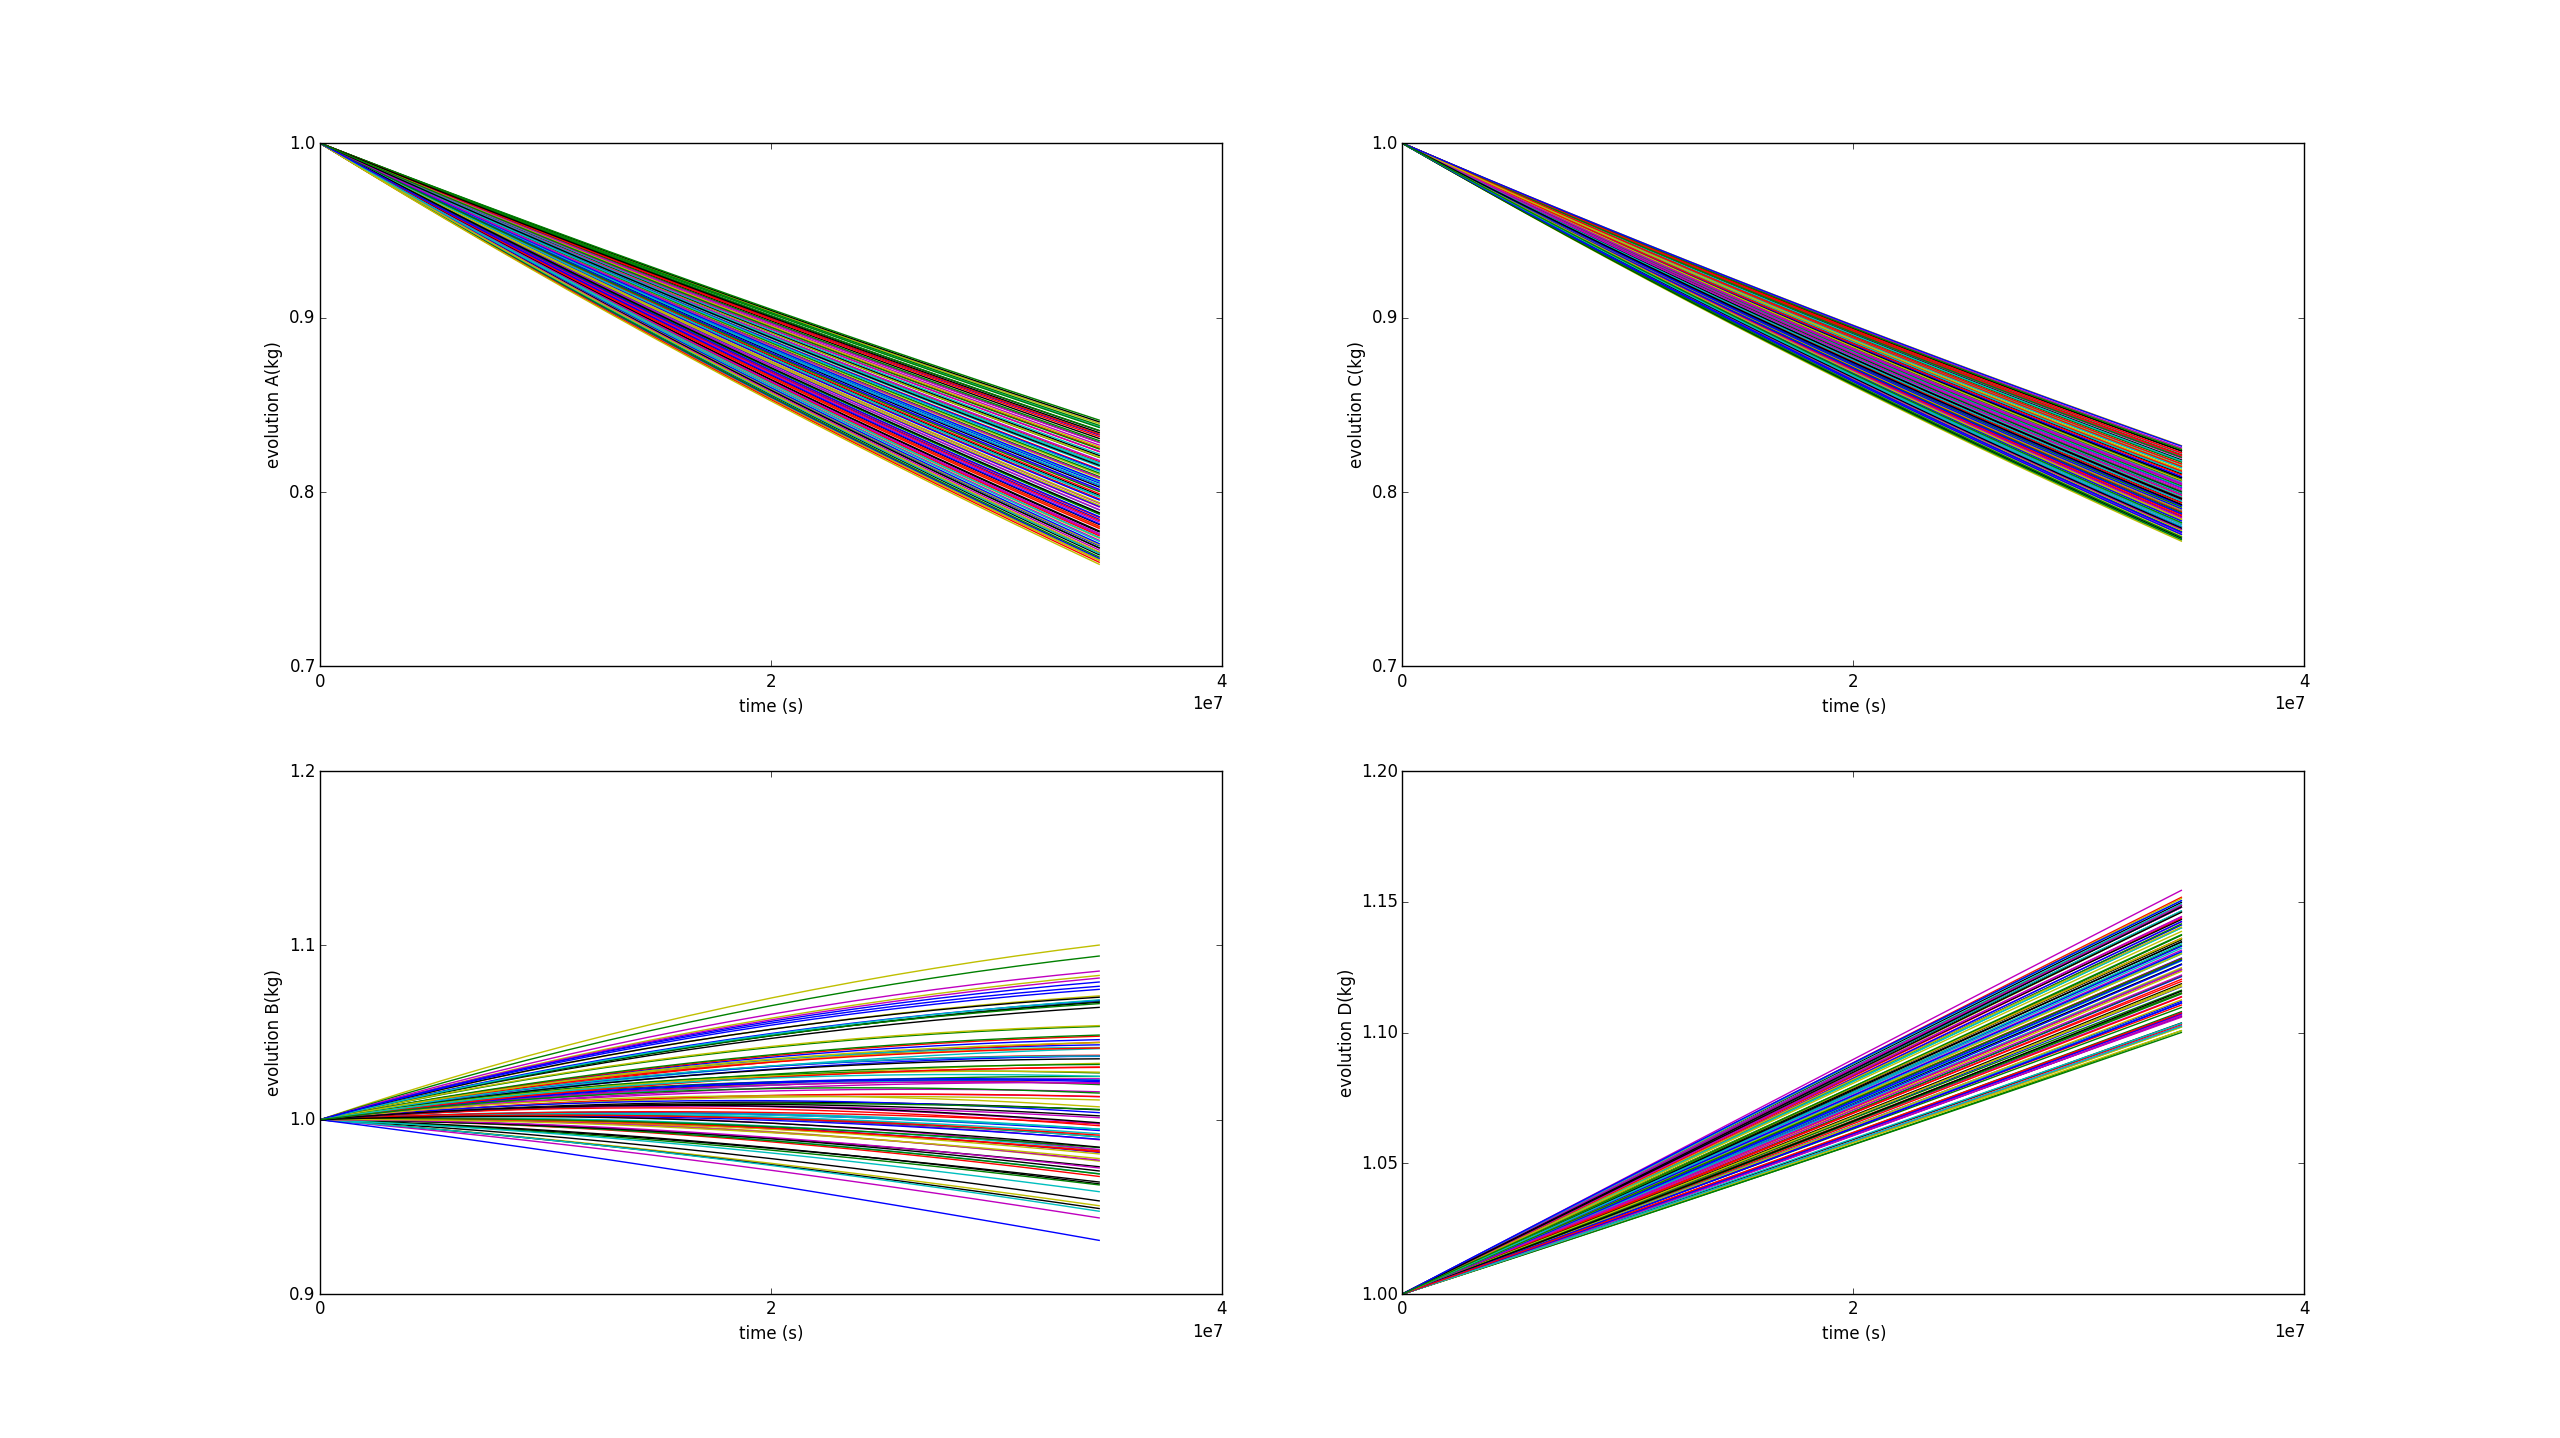
\includegraphics[scale=0.7]{pics/Stratified_histories.png}
  \caption{Plot of the histories generated by the Stratified sampling for variables $A,B,C,D$.}
  \label{fig:historiesStratifiedPlotLine}
 \end{figure}
 %%%%%%%%%%%%%%%%%%%%%%%%%%%%%%%%%%%%%%%%%%%%%%%%%%%%%%%%%%
  In this block, both the Out-Stream types are constructed: 
  \begin{itemize}
    \item \textit{Print}: 
     \begin{itemize}
       \item named ``samples'' connected with the \textit{DataObjects} \textbf{Entity} ``samples'' 
                (\xmlNode{source})
       \item named ``histories'' connected with the \textit{DataObjects} \textbf{Entity} ``histories'' (\xmlNode{source})          
     \end{itemize}         
      When these objects get used, all the information contained in the 
      linked  \textit{DataObjects} are going 
    to be dumped in CSV files (\xmlNode{type}).
    \item \textit{Plot}: 
    \begin{itemize}
      \item named ``historiesPlot'' connected with the  \textit{DataObjects} 
      \textbf{Entity} ``samples''.  This plot will draw the final state of the
      variables $A,B,C,D$ with respect to the input variables $sigma$(s) 
      and $decay$(s) . 
      \item named ``samplesPlot3D'' connected with the  
      \textit{DataObjects} \textbf{Entity} ``histories''. This plot will draw the 
      evolution of the variables $A,B,C,D$;
    \end{itemize}
     As it can be noticed, both plots are of type \textit{SubPlot}. Four plots
     are going to be placed in each of the figures.
  \end{itemize}   
   \item \textbf{\textit{Steps}}:   
\begin{lstlisting}[style=XML,morekeywords={arg,extension,pauseAtEnd,overwrite}]
  <Steps>
    <MultiRun name="sample">
      <Input 	    class="Files" 			 type="input">referenceInput.xml</Input>
      <Model 	    class="Models" 		 type="Code">testModel</Model>
      <Sampler 	class="Samplers" 		 type="Stratified">stratified</Sampler>
      <Output 	class="DataObjects"  type="PointSet">samples</Output>
      <Output 	class="DataObjects"  type="HistorySet">histories</Output>
    </MultiRun>
    <IOStep name="writeHistories" pauseAtEnd="True">
        <Input class="DataObjects" type="HistorySet">histories</Input>
        <Input class="DataObjects" type="PointSet">samples</Input>
        <Output 	class="OutStreamManager" type="Plot">samplesPlot3D</Output>
        <Output 	class="OutStreamManager" type="Plot">historyPlot</Output>
        <Output 	class="OutStreamManager" type="Print">samples</Output>
        <Output 	class="OutStreamManager" type="Print">histories</Output>
    </IOStep>
  </Steps>
\end{lstlisting}
 %%%%%%%%%%%%%%%%%%%%%%%%%%%%%%%%%%%%%%%%%%%%%%%%%%%%%%%%%%
 %figure samples
 \begin{figure}[h!]
  \centering
  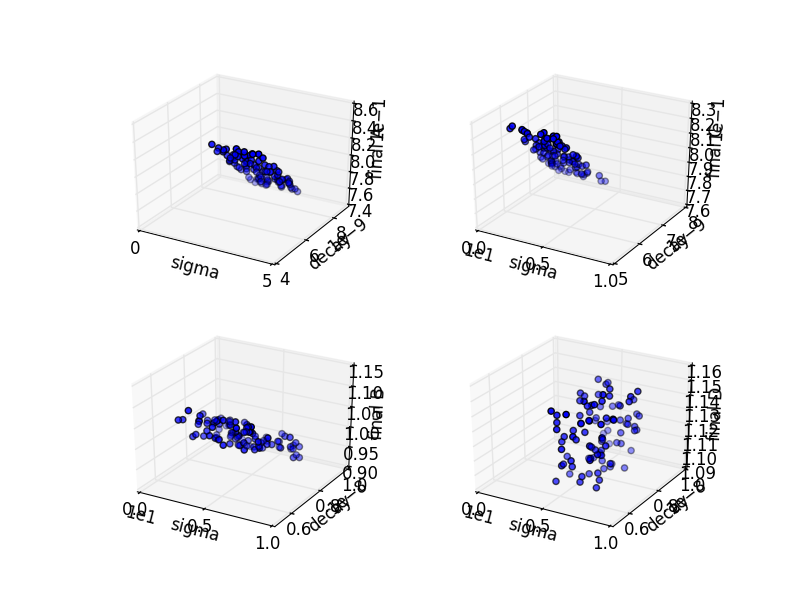
\includegraphics[scale=0.7]{pics/Stratified_pointsets.png}
  \caption{Plot of the samples generated by the Stratified sampling for variables $A,B,C,D$.}
  \label{fig:samplesStratifiedPlotLine}
 \end{figure}
 %%%%%%%%%%%%%%%%%%%%%%%%%%%%%%%%%%%%%%%%%%%%%%%%%%%%%%%%%%
   Finally, all the previously defined \textbf{Entities} can be combined in 
   the \xmlNode{Steps} block. As inferable, 
   two \xmlNode{Steps} have been inputted:
   \begin{itemize}
     \item \xmlNode{MultiRun} named ``sample'', used to run the multiple  
     instances of the driven code and 
     collect the outputs in the two \textit{DataObjects}. As it can be
     seen, the \xmlNode{Sampler} is inputted to communicate to the 
     \textit{Step} that the driven code needs to
     be perturbed through the Stratified sampling;
     \item  \xmlNode{IOStep} named ``writeHistories'', used to 1) dump 
     the ``histories'' and ``samples'' \textit{DataObjects} 
     \textbf{Entity} in a CSV file and 2) plot the data in the PNG file and 
     on the screen.
   \end{itemize}
\end{enumerate} 
 As previously mentioned, Figures~\ref{fig:historiesStratifiedPlotLine} and ~\ref{fig:samplesStratifiedPlotLine}  report the evolution of the 
 variables $A,B,C,D$ and their final values, respectively.

%%%%%%%%%%%%%%%%%%%%%%%%%

\subsection{Sparse Grid Collocation}
\label{sub:Stratified}
The Sparse Grid Collocation sampler represents an advanced methodology to perform Uncertainty Quantification. They aim
to explore the input space leveraging the information contained in the associated probability density functions. It builds on generic Grid sampling by selecting evaluation points based on characteristic quadratures as part of stochastic collocation for generalized polynomial chaos uncertainty quantification. In collocation an N-dimensional grid is constructed, with each uncertain variable providing an axis. Along each axis, the points of evaluation correspond to quadrature points necessary to integrate polynomials. In the simplest (and most naive) case, a N-Dimensional tensor product of all possible combinations of points from each dimension’s quadrature is constructed as sampling points. The number of necessary samples can be reduced by employing Smolyak-like sparse grid algorithms, which use reduced combinations of polynomial orders to reduce the necessary sampling space.
\\In this section, a brief theoretical 
background is reported. In addition,it is shown how to employ this methodology with RAVEN.
\subsubsection{Sparse Grid Collocation theory introduction}
\label{subsub:SGctheory}
\paragraph{Generalized Polynomial Chaos}
In general, polynomial chaos expansion (PCE) methods seek to interpolate the simulation code as a combination of
polynomials of varying degree in each dimension of the input space.  Originally Wiener
proposed expanding in Hermite polynomials for Gaussian-normal distributed variables~\cite{wiener}.  Askey and
Wilson generalized Hermite polynomials to include Jacobi polynomials, including Legendre and Laguerre
polynomials~\cite{Wiener-Askey}.  Xiu and Karniadakis combines these concepts to perform PCE for a range of Gaussian-based
distributions with corresponding polynomials,
including Legendre polynomials for uniform distributions, Laguerre polynomials for Gamma distributions, and
Jacobi polynomials for Beta distributions \cite{xiu}.

In each of these cases, a probability-weighted
integral over the distribution can be cast in a way that the corresponding polynomials are orthogonal over the
same weight and interval.  These chaos Wiener-Askey polynomials were used by Xiu and Karniadakis to develop
the generalized polynomial chaos expansion method (gPC), including a transformation for applying the same
method to arbitrary distributions (as long as they have a known inverse CDF)~\cite{xiu}.  Two significant
methodologies have grown from gPC application.  The first makes use of Lagrange polynomials to expand the
original function or simulation code, as they can be made orthogonal over the same domain as the
distributions~\cite{SCLagrange}; the other uses the Wiener-Askey polynomials~\cite{xiu}. 

Let's consider a simulation code that produces a quantity of interest $u$ as a function $u(Y)$ whose arguments are
the uncertain, distributed input
parameters $Y=(Y_1,\ldots,Y_n,\ldots,Y_N)$.  A particular realization $\omega$ of $Y_n$ is expressed by
$Y_n(\omega)$, and a single realization of the entire input space results in a solution to the function as
$u(Y(\omega))$. Obtaining a realization of $u(Y)$ may take considerable computation time and
effort.
$u(Y)$ gets expanded in orthonormal multidimensional polynomials $\Phi_k(Y)$, where $k$ is a multi-index tracking
the polynomial order in each axis of the polynomial Hilbert space, and $\Phi_k(Y)$ is constructed as
\begin{equation}\label{eq:gPC}
  \Phi_k(Y) = \prod_{n=1}^N \phi_{k_n}(Y_n),
\end{equation}
where $\phi_{k_n}(Y_n)$ is a single-dimension Wiener-Askey orthonormal polynomial of order $k_n$ and
$k=(k_1,\ldots,k_n,\ldots,k_N)$, $k_n\in\mathbb{N}^0$.  For example, given $u(y_1,y_2,y_3)$, $k=(2,1,4)$ 
is the multi-index of the
product of a second-order polynomial in $y_1$, a first-order polynomial in $y_2$, and a fourth-order
polynomial in $y_4$. The gPC for $u(Y)$ using this notation is
\begin{equation}
  u(Y) \approx \sum_{k\in\Lambda(L)} u_k\Phi_k(Y),
\end{equation}
where $u_k$ is a scalar weighting polynomial coefficient. The polynomials used in the expansion are determined
by the set of multi-indices $\Lambda(L)$, where $L$ is a truncation order.  In the limit
that $\Lambda$ contains all possible combinations of polynomials of any order, Eq. \ref{eq:gPC} is exact.
Practically, however, $\Lambda$ is truncated to some finite set of combinations, discussed in section
\ref{sec:indexSets}.

Using the orthonormal properties of the Wiener-Askey polynomials,
\begin{equation}
  \int_\Omega \Phi_k(Y)\Phi_{\hat k}(Y) \rho(Y) dY = \delta_{k\hat k},
\end{equation}
where $\rho(Y)$ is the combined PDF of $Y$, $\Omega$ is the multidimensional domain of $Y$, and $\delta_{nm}$
is the Dirac delta, we can isolate an expression of the polynomial expansion coefficients.
We multiply both sides of Eq. \ref{eq:gPC} by
$\Phi_{\hat k}(Y)$, integrate both sides over the probability-weighted input domain, and sum over all $\hat k$
to obtain the coefficients, sometimes referred to as polynomial expansion moments,
\begin{align}\label{eq:polycoeff}
  u_k &= \frac{\langle u(Y)\Phi_k(Y) \rangle}{\langle \Phi_k(Y)^2 \rangle},\\
      &= \langle u(Y)\Phi_k(Y) \rangle,
\end{align}
where we use the angled bracket notation to denote the probability-weighted inner product,
\begin{equation}
  \langle f(Y) \rangle \equiv \int_\Omega f(Y)\rho(Y) dY.
\end{equation}
When $u(Y)$ has an analytic form, these coefficients can be solved by integration; however, in general other
methods must be applied to numerically perform the integral.  While tools such as Monte Carlo integration can
be used to evaluate the integral, we can harness the properties of Gaussian quadratures because of the
probability weights and domain.  This stochastic collocation method is discussed in section \ref{sec:stoch
coll}.
\paragraph{Polynomial Index Set Construction}\label{sec:index sets}
The main concern in expanding a function in interpolating multidimensional polynomials is choosing appropriate polynomials to
make up the expansion.
There are many generic ways by which a polynomial set can be constructed.  Here  three static
approaches are presented: 
\begin{itemize}
  \item tensor product;
  \item total degree;
  \item hyperbolic cross.
\end{itemize}
In the nominal tensor
product case, $\Lambda(L)$ contains all possible combinations of polynomial indices up to truncation order $L$ in each
dimension, as
\begin{equation}
  \Lambda_\text{TP}(L)=\Big\{\bar p=(p_1,\cdots,p_N): \max_{1\leq n\leq N}p_n\leq L
\Big\}.
\end{equation}
The cardinality of this index set is $|\Lambda_\text{TP}(L)|=(L+1)^N$. For example, for a two-dimensional
input space ($N$=2) and truncation limit $L=3$, the index set $\Lambda_\text{TP}(3)$ is given in Table
\ref{tab:TP}, where the notation $(1,2)$ signifies the product of a polynomial that is first order in $Y_1$
and second order in $Y_2$.

\begin{table}[h]
  \centering
  \begin{tabular}{c c c c}
    (3,0) & (3,1) & (3,2) & (3,3) \\
    (2,0) & (2,1) & (2,2) & (2,3) \\
    (1,0) & (1,1) & (1,2) & (1,3) \\
    (0,0) & (0,1) & (0,2) & (0,3)
  \end{tabular}
  \caption{Tensor Product Index Set, $N=2,L=3$}
  \label{tab:TP}
\end{table}

It is evident there is some inefficiencies in this index set.  First, it suffers dramatically from the
\emph{curse of dimensionality}; that is, the number of polynomials required grows exponentially with
increasing dimensions.  Second, the total order of polynomials is not considered.  Assuming the contribution of
each higher-order polynomial is smaller than lower-order polynomials, the (3,3) term is
contributing sixth-order corrections that are likely smaller than the error introduced by ignoring
fourth-order corrections (4,0) and (0,4).  This leads to the development of the \emph{total degree} (TD) and
\emph{hyperbolic cross} (HC) polynomial index set construction strategies \cite{hctd}.

In TD, only multidimensional polynomials whose \emph{total} order at most $L$ are permitted,
\begin{equation}
  \Lambda_\text{TD}(L)=\Big\{\bar p=(p_1,\cdots,p_N):\sum_{n=1}^N p_n \leq L
\Big\}.
\end{equation}
The cardinality of this index set is $|\Lambda_\text{TD}(L)|={L+N\choose N}$, which grows with increasing
dimensions much more slowly than TP.  For the same $N=2,L=3$ case above, the TD index set is given in Table
\ref{tab:TD}. 

\begin{table}[h]
  \centering
  \begin{tabular}{c c c c}
    (3,0) &       &       &       \\
    (2,0) & (2,1) &       &       \\
    (1,0) & (1,1) & (1,2) &       \\
    (0,0) & (0,1) & (0,2) & (0,3)
  \end{tabular}
  \caption{Total Degree Index Set, $N=2,L=3$}
  \label{tab:TD}
\end{table}

In HC, the \emph{product} of polynomial orders is used to restrict allowed polynomials in the index set.  This
tends to polarize the expansion, emphasizing higher-order polynomials in each dimension but lower-order
polynomials in combinations of dimensions, as
\begin{equation}
  \Lambda_\text{HC}(L)=\Big\{\bar p=(p_1,\ldots,p_N):\prod_{n=1}^N p_n+1 \leq L+1
\Big\}.
\end{equation}
The cardinality of this index set is bounded by $|\Lambda_\text{HC}(L)|\leq (L+1)(1+\log(L+1))^{N-1}$. It
grows even more slowly than TD with increasing dimension, as shown in Table \ref{tab:HC} for $N=2,L=3$.

\begin{table}[h]
  \centering
  \begin{tabular}{c c c c}
    (3,0) &       &       &       \\
    (2,0) &       &       &       \\
    (1,0) & (1,1) &       &       \\
    (0,0) & (0,1) & (0,2) & (0,3)
  \end{tabular}
  \caption{Hyperbolic Cross Index Set, $N=2,L=3$}
  \label{tab:HC}
\end{table}

It has been shown that the effectiveness of TD and HC as index set choices depends strongly on the regularity
of the responce \cite{hctd}.  TD tends to be most effective for infinitely-continuous response surfaces,
while HC is more effective for surfaces with limited smoothness or discontinuities.

\paragraph{Anisotropy}
While using TD or HC to construct the polynomial index set combats the curse of dimensionality present in TP,
it is not eliminated and continues to be an issue for problems of large dimensionality.  Another method that can
be applied to mitigate this issue is index set anisotropy, or the unequal treatment of various dimensions.
In this strategy, weighting factors $\alpha=(\alpha_1,\ldots,\alpha_n,\ldots,\alpha_N)$ are applied in each
dimension to allow additional polynomials in some dimensions and less in others.  This change adjusts the TD
and HC construction rules as follows, where $|\alpha|_1$ is the one-norm of $\alpha$.
\begin{equation}
  \tilde\Lambda_{TD}(L)=\Big\{\bar p=(p_1,\ldots,p_N):\sum_{n=1}^{N} \alpha_n p_{n} \leq |\vec\alpha|_1 L\Big\},
\end{equation}
agagaag
\begin{equation}
  \tilde\Lambda_\text{HC}(L)=\Big\{\bar p=(p_1,\cdots,p_N):\prod_{n=1}^N (p_n+1)^{\alpha_n} \leq
  (L+1)^{|\vec\alpha|_1} \Big\}
\end{equation}
As it is desirable to obtain the isotropic case from a reduction of the anisotropic cases, let's define the
one-norm for the weights as
\begin{equation}
  |\alpha|_1 = \frac{\sum_{n=1}^N \alpha_n}{N}.
\end{equation}
Considering the same case above ($N=2,L=3$), it can be applied weights $\alpha_1=5,\alpha_2=3$, and the resulting index
sets are Tables \ref{tab:aniTD} (TD) and \ref{tab:aniHC} (HC).

\begin{table}[h]
  \centering
  \begin{tabular}{c c c c c}
    (2,0) &       &       &       & \\
    (1,0) & (1,1) & (1,2) &       & \\
    (0,0) & (0,1) & (0,2) & (0,3) & (0,4)
  \end{tabular}
  \caption{Anisotropic Total Degree Index Set, $N=2,L=3$}
  \label{tab:aniTD}
\end{table}

\begin{table}[h]
  \centering
  \begin{tabular}{c c c c}
    (1,0) &       &       &       \\
    (0,0) & (0,1) & (0,2) & (0,3)
  \end{tabular}
  \caption{Anisotropic Hyperbolic Cross Index Set, $N=2,L=3$}
  \label{tab:aniHC}
\end{table}

There are many methods by which anisotropy weights can be assigned.  Often, if a problem is well-known to an 
analyst, it may be enough to use heuristics to assign importance arbitrarily.  Otherwise, a smaller
uncertainty quantification solve can be used to roughly determine sensitivity coefficients (such as Pearson
coefficients), and the inverse of those can then be applied as anisotropy weights.  Sobol coefficients
obtained from first- or second-order HDMR, an additional sampling strategy present in RAVEN, could also serve as a basis for these weights.
A good choice of anisotropy weight can greatly speed up convergence; however, a
poor choice can slow convergence considerably, as computational resources are used to resolve low-importance
dimensions.

\paragraph{Stochastic Collocation}\label{sec:stoch coll}
Stochastic collocation is the process of using collocated points to approximate integrals of stochastic space
numerically.  In particular let's consider using Gaussian quadratures (Legendre, Hermite, Laguerre, and Jacobi)
corresponding to the polynomial expansion polynomials for numerical integration.  Quadrature integration takes
the form
\begin{align}
  \int_a^b f(x)\rho(x) &= \sum_{\ell=1}^\infty w_\ell f(x_\ell),\\
  &\approx \sum_{\ell=1}^{\hat L} w_\ell f(x_\ell),
\end{align}
where $w_\ell,x_\ell$ are corresponding points and weights belonging to the quadrature set, truncated at order
$\hat L$.  At this point, this $\hat L$ should not be confused with the polynomial expansion truncation order $L$.  This expression can be simplified using the operator notation
\begin{equation}\label{eq:quad op}
  q^{(\hat L)}[f(x)] \equiv \sum_{\ell=1}^{\hat L} w_\ell f(x_\ell).
\end{equation}
A nominal multidimensional quadrature is the tensor product of
individual quadrature weights and points, and can be written
\begin{align}
  Q^{(\vec{L})} &= q^{(\hat L_1)}_1 \otimes q^{(\hat L_2)}_2 \otimes \cdots,\\
                     &= \bigotimes_{n=1}^N q^{(\hat L_n)}_n.
\end{align}
It is worth noting each quadrature may have distinct points and weights; they need to not be constructed using
the same quadrature rule.
In general, one-dimensional Gaussian
quadrature excels in exactly integrating polynomials of order $2p-1$ using $p$ points and weights;
equivalently, it requires $(p+1)/2$ points to integrate an order $p$ polynomial. 
 
For convenience the coefficient integral to be evaluated is here reported again, Eq.
\ref{eq:polycoeff}.
\begin{equation}
  u_k = \langle u(Y)\Phi_k(Y) \rangle.
\end{equation}
This integral can be approximated with the appropriate Gaussian quadrature as
\begin{align}
  u_k &\approx Q^{(\vec{\hat L})}[u(Y)\Phi_k(Y)],
\end{align}
where bold vector notation is used to note the order of each individual quadrature,
$\vec{\hat L} = [\hat L_1, \ldots,\hat L_n,\ldots,\hat L_N]$. For clarity, the bold notation is removed and
it is assumed a one-dimensional problem, which extrapolates as expected into the multidimensional case.
\begin{align}
  u_k &\approx q^{(\hat L)}[u(Y)\Phi_k(Y)],\\
      &= \sum_{\ell=1}^{\hat L} w_\ell u(Y_\ell)\Phi_k(Y_\ell).
\end{align}
In order to determine the quadrature order $\hat L$ needed to accurately integrate this expression, let's consider the
gPC formulation for $u(Y)$ in Eq. \ref{eq:gPC} and replace it in the sum,
\begin{equation}
  u_k\approx \sum_{\ell=1}^{\hat L} w_\ell \Phi_k(Y_\ell) \sum_{k\in\Lambda(L)}u_{\hat k}\Phi_{\hat k}(Y_\ell).
\end{equation}
Using orthogonal properties of the polynomials, this reduces as $\hat L\to\infty$ to
\begin{equation}
  u_k\approx \sum_{\ell=1}^{\hat L} w_\ell u_k \Phi_k(Y_\ell)^2.
\end{equation}
Thus, the integral, to the same error introduced by truncating the  gPC expansion, the quadrature is
approximating an integral of order $2k$. As a result, the quadrature order should be order 
\begin{equation}
  p=\frac{2k+1}{2}=k+\frac{1}{2}<k+1,
\end{equation}
so it  can conservatively used  $p=k+1$.  In the case of the largest polynomials with order
$k=L$, the quadrature size $\hat L$ is the same as $L+1$.  It is worth noting that if $u(Y)$ is effectively of
much higher-order polynomial than $L$, this equality for quadrature order does not hold true; however, it also
means that gPC of order $L$ will be a poor approximation.

While a tensor product of highest-necessary quadrature orders could serve as a suitable multidimensional
quadrature set, we can make use of Smolyak-like sparse quadratures to reduce the number of function
evaluations necessary for the TD and HC polynomial index set construction strategies.

\paragraph{Smolyak Sparse Grids}
Smolyak sparse grids \cite{smolyak} are an attempt to discover the smallest necessary quadrature set to
integrate a multidimensional integral with varying orders of predetermined quadrature sets.  In RAVEN case, the
polynomial index sets determine the quadrature orders each one needs in each dimension to be integrated
accurately.  For example, the polynomial index set point (2,1,3) requires three points in $Y_1$, two in $Y_2$,
and four in $Y_3$,or
\begin{equation}
  Q^{(2,1,3)} = q^{(3)}_1 \otimes q^{(2)}_2 \otimes q^{(4)}_3.
\end{equation}
The full tensor grid of all collocation points would be the tensor product of all quadrature for all points,
or
\begin{equation}
  Q^{(\Lambda(L))} = \bigotimes_{k\in\Lambda}Q^{(k)}.
\end{equation}
Smolyak sparse grids consolidate this tensor form by adding together the points from tensor products of subset
quadrature sets.  Returning momentarily to a one-dimensional problem, let's introduce the notation
\begin{equation}
  \Delta_k^{(\hat L)}[f(x)] \equiv (q_k^{(\hat L)} - q_{k-1}^{(\hat L)})[f(x)],
\end{equation}
\begin{equation}
  q_0^{(\hat L)}[f(x)] = 0.
\end{equation}
A Smolyak sparse grid is then defined and applied to the desired integral in Eq. \ref{eq:polycoeff},
\begin{equation}
  S^{(\vec{\hat L})}_{\Lambda,N}[u(Y)\Phi_k(Y)] = \sum_{k\in\Lambda(L)} \left(\Delta_{k_1}^{(\hat L_1)} \otimes \cdots \otimes
  \Delta_{k_N}^{(\hat L_N)}\right)[u(Y)\Phi_k(Y)].
\end{equation}
Equivalently, and in a more algorithm-friendly approach,
\begin{equation}
  S^{(\vec{\hat L})}_{\Lambda,N}[u(Y)\Phi_k(Y)] = \sum_{k\in\Lambda(L)} c(k)\bigotimes_{n=1}^N
  q^{(\hat L_n)}_n[u(Y)\Phi_k(Y)]
\end{equation}
where
\begin{equation}
  c(k) = \sum_{\substack{j=\{0,1\}^N,\\k+j\in\Lambda}} (-1)^{|j|_1},
\end{equation}
using the traditional 1-norm for $|j|_1$.
The values for $u_k$ can then be calculated as
\begin{align}
  u_k &= \langle u(Y)\Phi_k(Y) \rangle,\\
      &\approx S^{(\vec{\hat L})}_{\Lambda,N}[u(Y)\Phi_k(Y)].
\end{align}
With this numerical method to determine coefficients,  a complete method for performing SCgPC
analysis in an algorithmic manner is obtained.
\subsubsection{Sparse Grid Collocation sampling through RAVEN}
\label{subsub:SGcsamplingExample}
The goals of this section are about learning how to:
 \begin{enumerate}
   \item Set up a Sparse Grid Collocation sampling for the construction of a suitable surrogate model of a driven code;
   \item Construct a GaussPolynomialRom surrogate model (training stage);
   \item Use the constructed GaussPolynomialRom surrogate model instead of the driven code.
\end{enumerate}  
In order to accomplish these tasks, the following RAVEN \textbf{Entities} (XML blocks in the input files) need to be defined:
\begin{enumerate}
   \item \textbf{\textit{RunInfo}}:
\begin{lstlisting}[style=XML,morekeywords={arg,extension,pauseAtEnd,overwrite}]
  <RunInfo>
    <JobName>ChapterVII-I/SparseGrid</JobName>
    <Sequence>sample,Ntrain,sampleROM,writeHistories</Sequence>
    <WorkingDir>ChapterVII-I/SparseGrid</WorkingDir>
    <batchSize>12</batchSize>
  </RunInfo>
\end{lstlisting}   
   As reported in section~\ref{sub:EntitiesAndFlow}, the \textit{RunInfo} \textbf{Entity} is intended to set up the analysis 
   that the user wants to perform. In this specific case, four steps (\xmlNode{Sequence}) are going to be sequentially run 
   using 12 processors (\xmlNode{batchSize}). 
   \item \textbf{\textit{Files}}:
\begin{lstlisting}[style=XML,morekeywords={arg,extension,pauseAtEnd,overwrite}]
  <Files>
    <Input name="referenceInput.xml" type="input">referenceInput.xml</Input>
  </Files>
\end{lstlisting}
   Since the driven code uses a single input file, in this section the original input is placed. As detailed in the user manual
   the attribute  \xmlAttr{name} represents the alias that is going to be used in all the other input blocks in order to refer to this file.
   \item \textbf{\textit{Models}}:
\begin{lstlisting}[style=XML,morekeywords={arg,extension,pauseAtEnd,overwrite}]
  <Models>
    <Code name="testModel" subType="GenericCode">
      <executable>../physicalCode/analyticalbateman/AnalyticalDplMain.py</executable>
      <clargs arg="python" type="prepend"/>
      <clargs arg="" extension=".xml" type="input"/>
      <clargs arg=" " extension=".csv" type="output"/>
      <prepend>python</prepend>
    </Code>
    <ROM name="NROM" subType="GaussPolynomialRom">
        <Target>A,B,C,D</Target>
        <Features>sigma-A,sigma-B,sigma-C,sigma-D,decay-A,decay-B,decay-C,decay-D</Features>
        <IndexSet>TotalDegree</IndexSet>
        <PolynomialOrder>3</PolynomialOrder>
        <Interpolation poly="Legendre" quad="Legendre">sigma-A</Interpolation>
        <Interpolation poly="Legendre" quad="Legendre">sigma-B</Interpolation>
        <Interpolation poly="Legendre" quad="Legendre">sigma-C</Interpolation>
        <Interpolation poly="Legendre" quad="Legendre">sigma-D</Interpolation>
        <Interpolation poly="Legendre" quad="Legendre">decay-A</Interpolation>
        <Interpolation poly="Legendre" quad="Legendre">decay-B</Interpolation>
        <Interpolation poly="Legendre" quad="Legendre">decay-C</Interpolation>
        <Interpolation poly="Legendre" quad="Legendre">decay-D</Interpolation>
    </ROM>
  </Models>
\end{lstlisting}
 As mentioned above, the goal of this example is the generation of a \text{GaussPolynomialRom} 
 for sub-sequential usage instead of the original code. Indeed, in addition to the previously explained Code model,
 the ROM of type \textit{GaussPolynomialRom} is here specified. The ROM will be generated through a Sparse Grid
 Collocation sampling strategy. All the 4 targets $A,B,C,D$ are going to be modeled through this ROM as function
 of the uncertain parameters $sigmas$ and $decays$.
   \item \textbf{\textit{Distributions}}:
\begin{lstlisting}[style=XML,morekeywords={arg,extension,pauseAtEnd,overwrite}]
  <Distributions>
      <Uniform name="sigmaA">
          <lowerBound>6.9</lowerBound>
          <upperBound>8.1</upperBound>
      </Uniform>
      <Uniform name="sigmaB">
          <lowerBound>3.9</lowerBound>
          <upperBound>5.1</upperBound>
      </Uniform>
      <Uniform name="sigmaC">
          <lowerBound>1.9</lowerBound>
          <upperBound>3.1</upperBound>
      </Uniform>
      <Uniform name="sigmaD">
          <lowerBound>0.9</lowerBound>
          <upperBound>1.1</upperBound>
      </Uniform>
      <Uniform name="decayConstantA">
          <lowerBound>0.0000000038</lowerBound>
          <upperBound>0.0000000052</upperBound>
      </Uniform>
      <Uniform name="decayConstantB">
          <lowerBound>0.0000000058</lowerBound>
          <upperBound>0.0000000072</upperBound>
      </Uniform>
      <Uniform name="decayConstantC">
          <lowerBound>0.0000000068</lowerBound>
          <upperBound>0.0000000082</upperBound>
      </Uniform>
      <Uniform name="decayConstantD">
          <lowerBound>0.0000000078</lowerBound>
          <upperBound>0.0000000092</upperBound>
      </Uniform>
  </Distributions>
\end{lstlisting}
  In the Distributions XML section, the stochastic model for the 
  uncertainties  treated by the Sparse Grid Collocation sampling are reported. In 
  this case 8 distributions are defined: 
  \begin{itemize}
    \item $sigmaA \sim \mathbb{U}(6.9,8.1)$, used to model the uncertainty 
    associated with  the Model \textit{sigma-A};
    \item $sigmaB \sim \mathbb{U}(3.9,5.1)$, used to model the uncertainty 
    associated with  the Model \textit{sigma-B};
    \item $sigmaC \sim \mathbb{U}(1.9,3.1)$, used to model the uncertainty 
    associated with  the Model \textit{sigma-C};
    \item $sigmaD \sim \mathbb{U}(0.9,1.1)$, used to model the uncertainty 
    associated with  the Model \textit{sigma-D};
    \item  $decayConstantA \sim \mathbb{U}(3.8e-9,5.2e-9)$,  used to 
    model the uncertainty 
    associated with  the Model \textit{decay-A}.
    \item  $decayConstantB \sim \mathbb{U}(5.8e-9,7.2e-9)$,  used to 
    model the uncertainty 
    associated with  the Model \textit{decay-B}.
    \item  $decayConstantC \sim \mathbb{U}(6.8e-9,8.2e-9)$,  used to 
    model the uncertainty 
    associated with  the Model \textit{decay-C}.
    \item  $decayConstantD \sim \mathbb{U}(7.8e-9,9.2e-9)$,  used to 
    model the uncertainty 
    associated with  the Model \textit{decay-D}.
  \end{itemize}
   \item \textbf{\textit{Samplers}}:
\begin{lstlisting}[style=XML,morekeywords={arg,extension,pauseAtEnd,overwrite}]
  <Samplers>
    <SparseGridCollocation name="NSG" parallel="1">
      <variable name="sigma-A">
        <distribution>sigmaA</distribution>
      </variable>
      <variable name="sigma-B">
          <distribution>sigmaB</distribution>
      </variable>
      <variable name="sigma-C">
          <distribution>sigmaC</distribution>
      </variable>
      <variable name="sigma-D">
          <distribution>sigmaD</distribution>
      </variable>
      <variable name="decay-A">
          <distribution>decayConstantA</distribution>
      </variable>
      <variable name="decay-B">
          <distribution>decayConstantB</distribution>
      </variable>
      <variable name="decay-C">
          <distribution>decayConstantC</distribution>
      </variable>
      <variable name="decay-D">
          <distribution>decayConstantD</distribution>
      </variable>
      <ROM class="Models" type="ROM">NROM</ROM>
    </SparseGridCollocation>
  </Samplers> 
\end{lstlisting}
  In order to employ the Sparse Grid Collocation sampling strategy, a 
  \xmlNode{SparseGridCollocation} node needs to be inputted. 
  As it can be
  seen from above, each variable is associated to a different distribution,
  defined in the  \xmlNode{Distributions} block.
  In addition, the \textit{GaussPolynomialRom}  \xmlNode{ROM} is inputted. The setting of this ROM (e.g. polynomial order, Index set method, etc.) determines how the Stochastic Collocation Method is 
  employed.
   \item \textbf{\textit{DataObjects}}:
\begin{lstlisting}[style=XML,morekeywords={arg,extension,pauseAtEnd,overwrite}]
  <DataObjects>
    <PointSet name="inputPlaceHolder">
      <Input>sigma-A,sigma-B,sigma-C,sigma-D,decay-A,decay-B,decay-C,decay-D</Input>
      <Output>OutputPlaceHolder</Output>
    </PointSet>
    <PointSet name="samples">
      <Input>sigma-A,sigma-B,sigma-C,sigma-D,decay-A,decay-B,decay-C,decay-D</Input>
      <Output>A,B,C,D,time</Output>
    </PointSet>
    <PointSet name="samplesROM">
        <Input>sigma-A,sigma-B,sigma-C,sigma-D,decay-A,decay-B,decay-C,decay-D</Input>
        <Output>A,B,C,D</Output>
    </PointSet>
    <HistorySet name="histories">
        <Input>sigma-A,sigma-B,sigma-C,sigma-D,decay-A,decay-B,decay-C,decay-D</Input>
        <Output>A,B,C,D,time</Output>
    </HistorySet>
  </DataObjects>
\end{lstlisting}
  Int this block, four \textit{DataObjects} are defined: 1) PointSet named 
  ``samples'' used to collect the final outcomes of the code, 2) HistorySet named ``histories'' in which the full time responses of the variables $A,B,C,D$ are going to be stored, 3) PointSet named    
  ``inputPlaceHolder'' used as input of the sampling applied on the constructed ROM and 4) PointSet named ``samplesROM'' used to collect the final outcomes of the ROM perturbations.
 %%%%%%%%%%%%%%%%%%%%%%%%%%%%%%%%%%%%%%%%%%%%%%%%%%%%%%%%%%
 %%%%%%%%%%%%%%%%%%%%%%%%%%%%%%%%%%%%%%%%%%%%%%%%%%%%%%%%%%
 %figure samples
 \begin{figure}[h!]
  \centering
  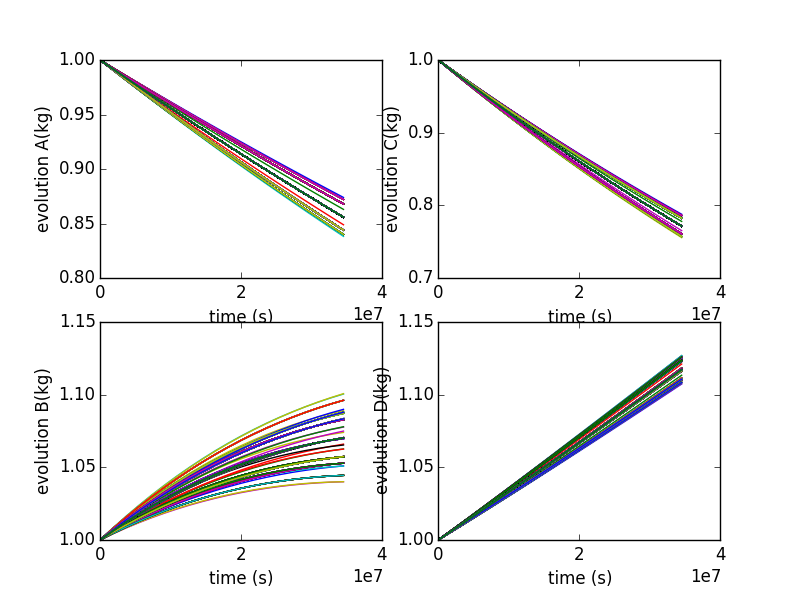
\includegraphics[scale=0.7]{pics/histories_SparseGrid.png}
  \caption{Plot of the samples generated by the Stratified sampling for variables $A,B,C,D$.}
  \label{fig:historiesSparseGridPlotLine}
 \end{figure}
 %%%%%%%%%%%%%%%%%%%%%%%%%%%%%%%%%%%%%%%%%%%%%%%%%%%%%%%%%%
 %%%%%%%%%%%%%%%%%%%%%%%%%%%%%%%%%%%%%%%%%%%%%%%%%%%%%%%%%%  
   \item \textbf{\textit{Steps}}:   
\begin{lstlisting}[style=XML,morekeywords={arg,extension,pauseAtEnd,overwrite}]
  <Steps>
    <MultiRun name="sample">
      <Input class="Files" type="input">referenceInput.xml</Input>
      <Model class="Models" type="Code">testModel</Model>
      <Sampler class="Samplers" type="SparseGridCollocation">NSG</Sampler>
      <Output class="DataObjects" type="PointSet">samples</Output>
      <Output class="DataObjects" type="HistorySet">histories</Output>
    </MultiRun>
    <RomTrainer name="Ntrain">
        <Input class="DataObjects" type="PointSet">samples</Input>
        <Output class="Models" type="ROM">NROM</Output>
    </RomTrainer>
    <MultiRun name="sampleROM" pauseAtEnd="false">
        <Input class="DataObjects" type="PointSet">inputPlaceHolder</Input>
        <Model class="Models" type="ROM">NROM</Model>
        <Sampler class="Samplers" type="SparseGridCollocation">NSG</Sampler>
        <Output class="DataObjects" type="PointSet">samplesROM</Output>
    </MultiRun>
    <IOStep name="writeHistories" pauseAtEnd="True">
        <Input class="DataObjects" type="HistorySet">histories</Input>
        <Input class="DataObjects" type="PointSet">samples</Input>
        <Input class="DataObjects" type="PointSet">samplesROM</Input>
        <Output 	class="OutStreamManager" type="Plot">samplesPlot3D</Output>
        <Output 	class="OutStreamManager" type="Plot">historyPlot</Output>
        <Output 	class="OutStreamManager" type="Plot">samplesROMPlot3D</Output>
        <Output 	class="OutStreamManager" type="Print">samples</Output>
        <Output 	class="OutStreamManager" type="Print">samplesROM</Output>
        <Output 	class="OutStreamManager" type="Print">histories</Output>
    </IOStep>
  </Steps>
\end{lstlisting}
  %%%%%%%%%%%%%%%%%%%%%%%%%%%%%%%%%%%%%%%%%%%%%%%%%%%%%%%%%%
 %figure samples
 \begin{figure}[h!]
  \centering
  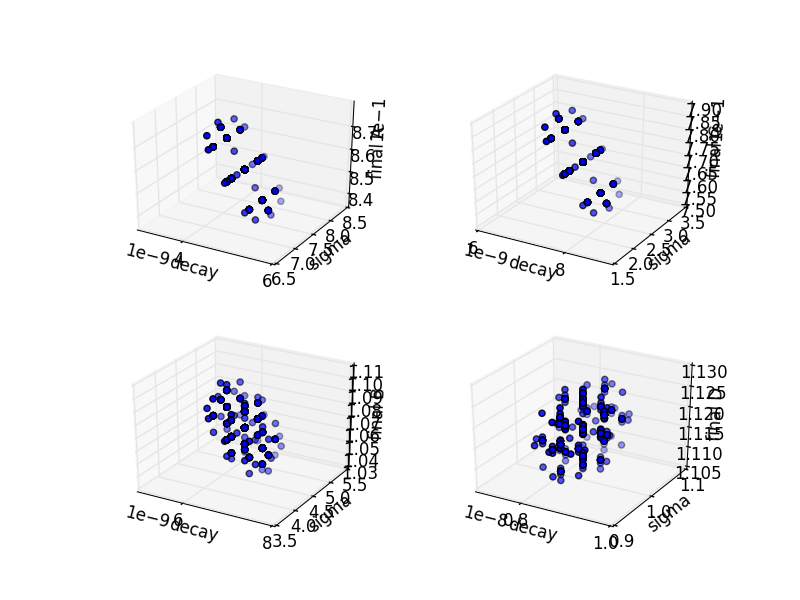
\includegraphics[scale=0.7]{pics/samples_SparseGrid.png}
  \caption{Plot of the samples generated by the Stratified sampling for variables $A,B,C,D$.}
  \label{fig:samplesSparseGridPlotLine}
 \end{figure}
 %%%%%%%%%%%%%%%%%%%%%%%%%%%%%%%%%%%%%%%%%%%%%%%%%%%%%%%%%%
   Finally, all the previously defined \textbf{Entities} can be combined in 
   the \xmlNode{Steps} block. As inferable, 
   4 \xmlNode{Steps} have been inputted:
   \begin{itemize}
     \item \xmlNode{MultiRun} named ``sample'', used to run the multiple  
     instances of the driven code and 
     collect the outputs in the two \textit{DataObjects}. As it can be
     seen, the \xmlNode{Sampler} is inputted to communicate to the 
     \textit{Step} that the driven code needs to
     be perturbed through the Sparse Grid Collocation  sampling;
     \item \xmlNode{RomTrainer} named ``Ntrain'', used to train (i.e. 
     construct) the Gauss Polynomial ROM. This step is essential if the
     user want to use the ROM in later steps;
     \item \xmlNode{MultiRun} named ``sampleROM'', used to run the multiple  
     instances of the previously constructed ROM and 
     collect the outputs in the \textit{samplesROM} \textit{DataObjects}.  
     As it can be seen, the same Sparse Grid Collocation sampler is
     here used.
     \item  \xmlNode{IOStep} named ``writeHistories'', used to 1) dump 
     the ``histories'', ``samples'' and ``samplesROM'' \textit{DataObjects} 
     \textbf{Entity} in a CSV file and 2) plot the data in the PNG file and 
     on the screen.
   \end{itemize}
\end{enumerate} 
 As previously mentioned, Figure~\ref{fig:historiesSparseGridPlotLine} 
 shows the evolution of the outputs $A,B,C,D$ under uncertainties. 
 Figures~\ref{fig:samplesSparseGridPlotLine} and 
 \ref{fig:samplesROMSparseGridPlotLine} show the final responses 
 of the sampling employed using the driven code and the ROM, 
 respectively. As it can be seen, the constructed ROM can perfectly
 represent the response of the driven code. This example shows the
 potential of reduced order modeling, in general, and of the 
 \textit{GaussPolynomialRom}, in particular.
 
  %%%%%%%%%%%%%%%%%%%%%%%%%%%%%%%%%%%%%%%%%%%%%%%%%%%%%%%%%%
 %figure samples
 \begin{figure}[h!]
  \centering
  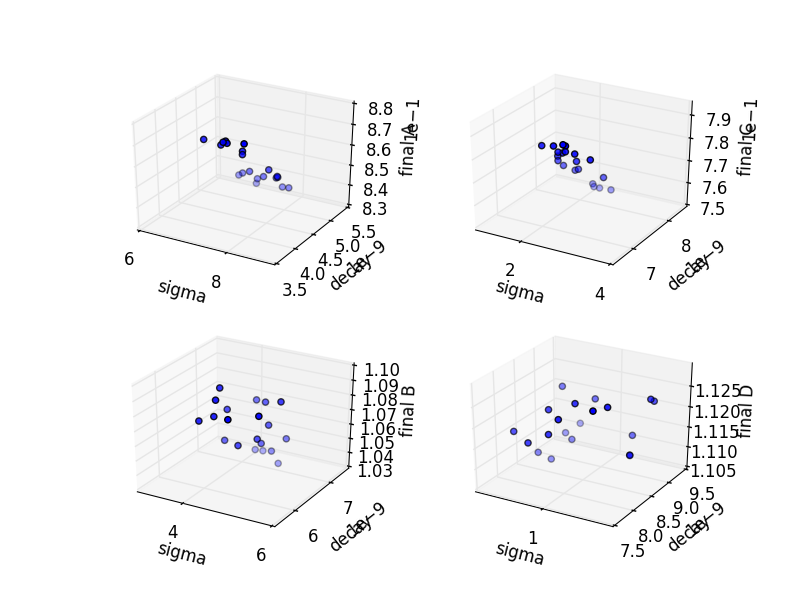
\includegraphics[scale=0.7]{pics/samplesROM_SparseGrid.png}
  \caption{Plot of the samples generated by the Stratified sampling for variables $A,B,C,D$.}
  \label{fig:samplesROMSparseGridPlotLine}
 \end{figure}
 %%%%%%%%%%%%%%%%%%%%%%%%%%%%%%%%%%%%%%%%%%%%%%%%%%%%%%%%%%









\section{Adaptive Sampling Strategies}
Performing UQ and Dynamic PRA can be
challenging from a computational point of view. The \textit{Forward}
sampling strategies reported in the previous Section can lead to a large number of
unnecessary evaluations of the physical model leading to an unacceptable resource expenses (CPU time).
In addition, the \textit{Forward} methodologies are not designed to leverage the information
content that is extractable from the simulations already concluded.

To overcome these limitations, in RAVEN several adaptive algorithms are available:
\begin{enumerate}
  \item \textit{Limit Surface Search}
  \item \textit{Adaptive Dynamic Event Tree}
  \item \textit{Adaptive Hybrid Dynamic Event Tree}
  \item \textit{Adaptive Sparse Grid}
  \item \textit{Adaptive Sobol Decomposition}.
\end{enumerate}
In this Section, only the first algorithm is going to be reported, explaining the theory behind it
and providing RAVEN examples.

%%%%%%%%%%%%%%%%%%%%%%%%%%%%%%%%
%%%%%%%%  Limit Surface Search %%%%%%%%
%%%%%%%%%%%%%%%%%%%%%%%%%%%%%%%%
\subsection{Limit Surface Search Method}
\label{sub:LS}
The motivation behind the choice of adaptive sampling strategies is that numerical
simulations are often computationally expensive, time consuming, and
with a large number of uncertain parameters. Thus, exploring the space
of all possible simulation outcomes is almost unfeasible using finite
computing resources. During DPRA analysis, it is
important to discover the relationship between a potentially large
number of uncertain parameters and the response of a simulation using
as few simulation trials as possible.
This is a typical context where ``goal'' oriented sampling could be
beneficial. The ``Limit
Surface Search method'' is a scheme  where few observations, obtained
from the model run, are used to build a simpler and computationally faster
mathematical representation of the model, ROM, also
known as Surrogate Model (ROM or SM). The ROM (see Section \ref{sec:ROMsTheory}) is then
used to predict where further exploration of the input space could be
most informative. This information is used to select new locations in the
input space for which a code run is executed (see
Figure~\ref{fig:ExampleLSschematic}). The new
observations are used to update the ROM and this process iterates
until, within a certain metric, it is converged.
\begin{figure}[h!]
  \centering
  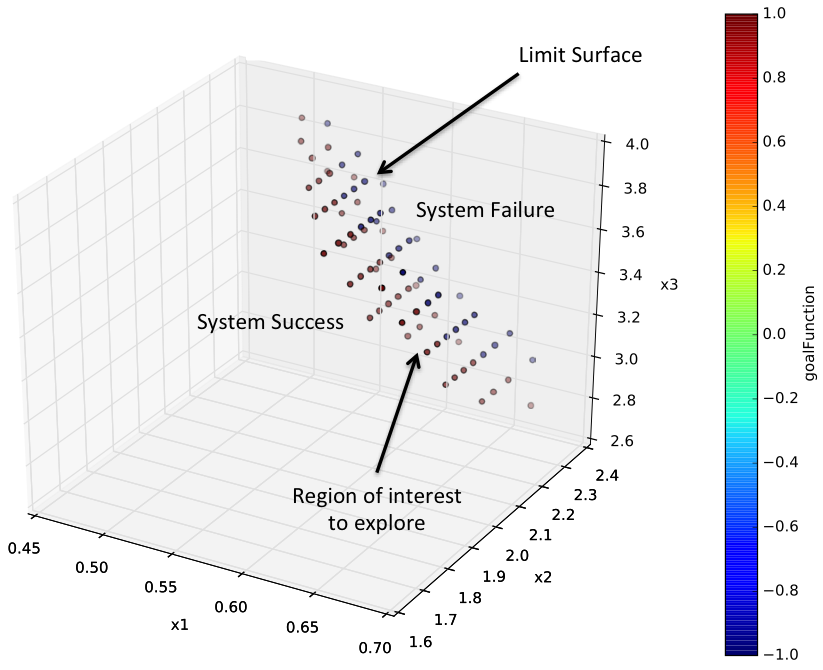
\includegraphics[width=1.0\textwidth]  {pics/ExampleLSschematic.png}
  \caption{Example of limit surface in the uncertain space.}
  \label{fig:ExampleLSschematic}
\end{figure}

In the case of the ``Limit
Surface (LS) Search method'', a ROM is used to
determine the location in the input space where further observations are most
informative to establish the location of the LS, then code runs are
executed on those locations and the ROM updated. The process
continues until the location of the LS is established within a certain tolerance.

%%%%%%%%%
%%%%%%%%% Limit Surface Concept and Properties
%%%%%%%%%
\subsubsection{Limit Surface Theory}
\label{sec:LSconcept}

To properly explain the LS concept and relative properties,
it is necessary to analyze the idea behind the LSs, firstly, from a
mathematical and, secondly, from a practical point of view.
Consider a dynamic system that is represented in the phase space by the Eq.~\ref{eq:dThetaOverDT} in Section~\ref{sec:RAVENconcept}.
The equation can be rewritten as follows:
\begin{equation}
\label{eq:ThetaXPT}
\frac{\partial \overline{\theta} }{\partial t}=\overline{H}\left (  \overline{x},\overline{p},t \right )
\end{equation}
where:
\begin{itemize}
  \item $\overline{\theta}$ represents the coordinate of the system in the
  phase space
  \item $\left (  \overline{x},\overline{p},t \right )$ independent variables
  that are separated, respectively, in spatial, temporal, and parametric
  space (distinction between $\left (  \overline{x},\overline{p},t \right )$ is purely based on engineering considerations).
\end{itemize}
Now it is possible to introduce the concept of ``goal'' function, $C$. $C$
is a binary function that, based on the response of the system, can
assume the value $0$ (false) to indicate that the system is properly
available (e.g., system success) and $1$ (true) to indicate that the
system is not available (e.g., failure of the system):
\begin{equation}
C\left (\overline{\theta}, \overline{x},\overline{p},t \right ) = C\left (H\left(\overline{x},\overline{p},t \right), \overline{x},\overline{p},t \right ) = C\left ( \overline{x},\overline{p},t \right )
\end{equation}
Without loss of generality, lets assume
that $C$ does not depend on time (e.g. $C\leftarrow
\bigintssss_{t_{0}}^{t_{end}}dtC\left(  \overline{x},\overline{p},t \right )$):
\begin{equation}
  \label{eq:goalFunction}
  C = C\left (\overline{x},\overline{p}\right )
\end{equation}
To simplify the mathematical description of the LS concept, it is
possible to hypothesize that the
equation describing the PDF time evolution of the system in the phase
space is of type Gauss
Codazzi (in its Liouville’s derivation)~\cite{MathFrameworkMC2013}, which allows ensuring that all the
stochastic phenomena in
the system are representable as PDFs in the uncertain domain
(see Section~\ref{sec:RAVENconcept}),. This allows combining the
parametric space with the initial condition space:
\begin{equation}
  \label{eq:goalFunctionCodazzi}
  \begin{matrix}
  \left ( \overline{x} \right ) \leftarrow \left ( \overline{x},\overline{p} \right ) \\
  C\left ( \overline{x} \right ) \leftarrow C\left ( \overline{x},\overline{p} \right )
  \end{matrix}
\end{equation}

This assumption is rarely violated, for example for those systems that
present an intrinsic
stochastic behavior (e.g., the dynamic of a particle of dust in the air
where it continuously and
randomly interacts with the molecules of air that ``move'' with different velocities and in different
and random directions). In most of the cases of interest in the safety analysis, the above
mentioned assumption is correct. The full heuristic approach to the characterization of system stochastic behaviors is reported in Section~\ref{sec:RAVENconcept}.
\\Under the above simplifications, it is possible to identify the region of the input space ($V$)
leading to a specific outcome of the ``goal'' function. For example, it can be defined
the failure region $V_{F}$ as the region of the input space where $C=1$:
\begin{equation}
 \label{eq:failureRegion}
V_{F}=\left \{ \forall \overline{x} | C\left ( \overline{x} \right ) = 1 \right \}
\end{equation}
The definition of the complementary of the failure region is obviously:
\begin{equation}
V_{F}^{c}=\left \{ \forall \overline{x} | C\left ( \overline{x} \right ) = 0 \right \}
\end{equation}
Its boundary is the named LS:
\begin{equation}
L_{S}= \partial V_{F}^{c}= \partial      \left \{ \forall \overline{x} | C\left ( \overline{x} \right ) = 1 \right \}
\end{equation}

The identification of the LS location is necessary to identify boundary regions for which the system under consideration will or will not exceed certain FOMs (e.g., operative margins).
\\The LS location is extremely important for design optimization and, in addition, its informative content can be used to analyze the system to characterize its behavior from a stochastic point of view. Consider $\overline{x} \in V$ and $\overline{x}\sim \overline{X}$,
where $\overline{x}$ is the random variate realization of the stochastic variable $\overline{X}$.
If $pdf_{\overline{X}}\left ( \overline{x} \right ) $ is the probability density function of $ \overline{X}$, the failure probability of the system $\left ( P_{F} \right )$ is:
\begin{equation}
\label{eq:probabilityFailure}
P_{F} = \bigintssss_{V}d\overline{x}C\left ( \overline{x} \right )pdf_{\overline{X}}\left ( \overline{x} \right ) = \bigintssss_{V_{F}+V_{F}^{c}}d\overline{x}C\left ( \overline{x} \right )pdf_{\overline{X}}\left ( \overline{x} \right )
\end{equation}
And, based on the definition given in Equations~\ref{eq:goalFunctionCodazzi} and \ref{eq:failureRegion}:
\begin{equation}
 \label{eq:failureProbIntegral}
 \bigintssss_{V_{F}}d\overline{x}pdf_{\overline{X}}\left ( \overline{x} \right )
 \end{equation}
Equations \ref{eq:probabilityFailure} and \ref{eq:failureProbIntegral} are summarized by stating that the system failure probability is
equivalent to the probability of the system being in the uncertain
subdomain (region of the input space) that leads to a failure pattern.
This probability is equal to the probability-weighted hyper-volume that is surrounded by the LS (see Figure ~\ref{fig:ProbabilityFailureLSExample}).
\begin{figure}[h!]
  \centering
  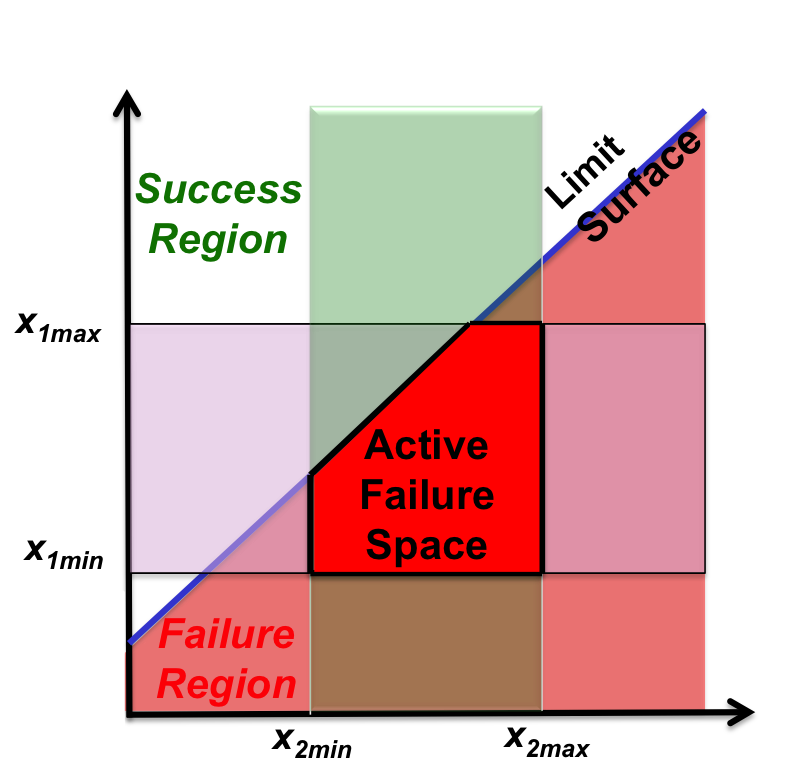
\includegraphics[width=1.0\textwidth]  {pics/ProbabilityFailureLSExample.png}
  \caption{Example of limit surface probability of failure region.}
  \label{fig:ProbabilityFailureLSExample}
\end{figure}
\\It is beneficial for better understanding to assess the LS concept through an example related to the safety of an Nuclear Power Plant (NPP).
As an example, consider a station black out (SBO) scenario in an NPP. Suppose that the only uncertain parameters are:
\begin{itemize}
  \item $t_{F}$: Temperature that would determine the failure of the fuel cladding
  \item $rt_{DGs}$: Recovery time of the diesel generators (DGs) that
  can guarantee, through the emergency core cooling system (ECCS),
  the removal of the decay heat.
\end{itemize}
And, the corresponding CDF (uniform) is:

\begin{equation}
t_{F}\sim pdf_{T_{F}}\left ( T_{F} \right )=\left\{\begin{matrix}
0 & if \: t_{F}< t_{F_{min}} \\
\frac{1}{\left ( t_{F_{max}}- t_{F_{min}} \right )=\Delta t_{F}} & \\
0 & if \: t_{F}>  t_{F_{max}}
\end{matrix}\right.
\end{equation}
%
%
\begin{equation}
rt_{DGs}\sim pdf_{RT_{DGs}}\left ( rt_{DGs} \right )=\left\{\begin{matrix}
0 & if \: rt_{DGs}<rt_{DGs_{min}}   \\
\frac{1}{\left ( rt_{DGs_{max}} - rt_{DGs_{min}} \right )=\Delta rt_{DGs}} & \\
0 & if \: rt_{DGs}>rt_{DGs_{max}}
\end{matrix}\right.
\end{equation}
For simplicity, assume that the clad temperature is a quadratic function of the DG recovery time in an SBO scenario:
\begin{equation}
  t = t_{0}+\alpha \times rt_{DGs}^{2}
\end{equation}
and that the  $ t_{F_{min}} > t_{0}+\alpha \times rt_{DGs_{min}}^{2}$
and $t_{F_{max}} < t_{0}+\alpha \times rt_{DGs_{max}}^{2}$.
The LS, failure region, and active part of the failure region (failure region with non-zero probability) are illustrated, for example, in Figure~\ref{fig:ProbabilityFailureLSExample} (in agreement with the above assumptions).
\begin{figure}[h!]
  \centering
  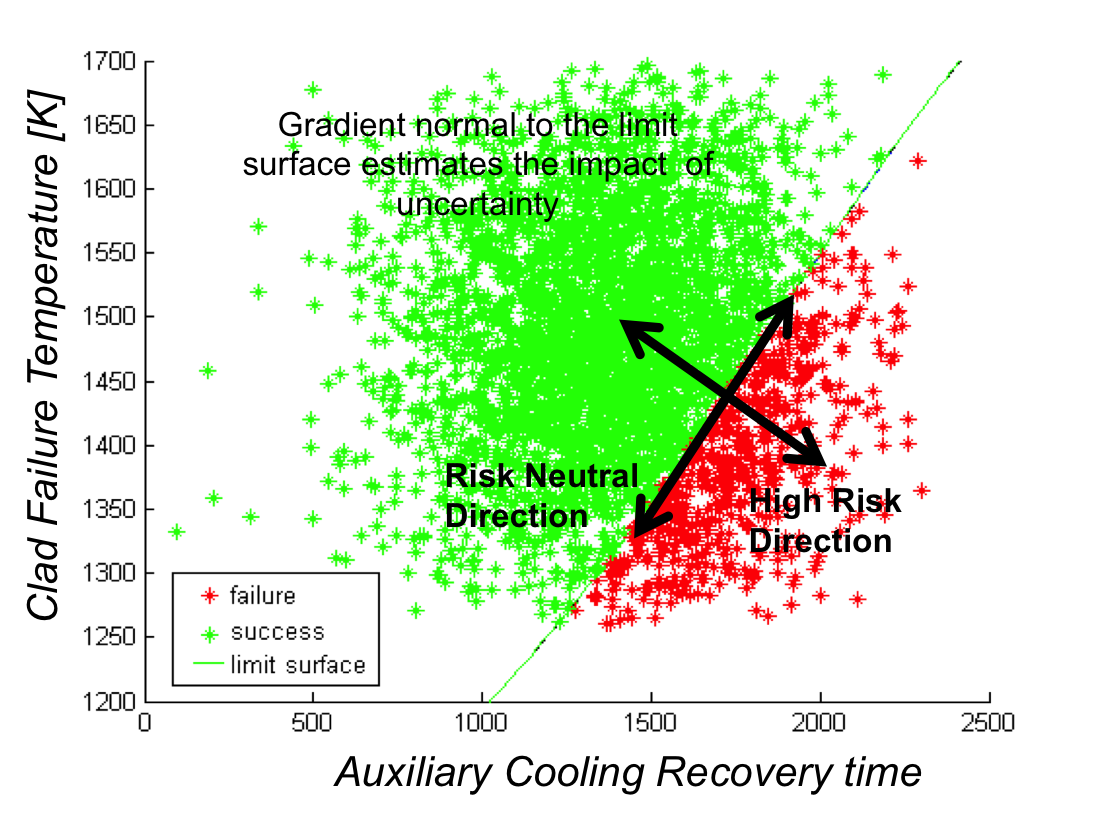
\includegraphics[width=1.0\textwidth]  {pics/ExampleLSwitRiskDirections.png}
  \caption{Example of limit surface highlighting the risk directions.}
  \label{fig:ExampleLSwitRiskDirections}
\end{figure}
In this case, the transition/failure probability is evaluated as follows:
\begin{equation}
\begin{matrix}
P_{F} = \bigintssss_{V_{F}}d\overline{x}\: pdf_{\overline{X}}\left ( \overline{x} \right )
= \bigintssss_{0}^{+\infty }d\overline{t_{F}}\: pdf_{T_{F}}\left ( T_{F} \right )\: \: \bigintssss_{\sqrt{\frac{t_{F}-t_{0}}{\alpha}}}^{+\infty } d\, rt_{DGs} \: pdf_{RT_{DGs}}\left ( rt_{DGs} \right )  =
\\
= \bigintssss_{t_{F_{min}}}^{t_{F_{max}}} dt_{F}\frac{1}{t_{F_{max}}-t_{F_{min}}}\: \: \bigintssss_{\sqrt{\frac{t_{F}-t_{0}}{\alpha}}}^{ rt_{DGs_{max}}}\: d\, rt_{DGs} \frac{1}{rt_{DGs_{max}}-rt_{DGs_{min}}} =
\\
= \frac{rt_{DGs_{max}}}{\Delta rt_{DGs}} + \frac{2\alpha}{3\left ( \Delta rt_{DGs}\Delta t_{F} \right )}
\left ( \sqrt[3/2]{\frac{t_{F_{min}}-t_{0}}{\alpha}} - \sqrt[3/2]{\frac{t_{F_{max}}-t_{0}}{\alpha}} \right )
\end{matrix}
\end{equation}

This simple example is useful to understand how the LS is defined in a practical application (that is analyzed numerically in the results Section) and how the hyper volume needs weighted with respect to the probability in the uncertain domain. An example of the computed LS is shown in Figure ~\ref{fig:ExampleLSwitRiskDirections}.
In this figure the neutral and high risk directions are highlighted.

%%%%%%%%%
%%%%%%%%% Limit Surface Search Algorithm
%%%%%%%%%
\paragraph{Limit Surface Search Algorithm}
\label{par:LSSalgorithm}
The identification of the LS location is extremely challenging,
depending on the particular physics/phenomena that are investigated.
To identify the real location of the LS, the evaluation of system
responses is needed, through the high-fidelity code (RELAP 7,
RELAP5-3D, etc.), in the full domain of uncertainty (infinite number of
combinations of uncertainties represented by the respective PDFs).
Obviously, this is not a feasible approach, and a reasonable
approximation is to locate the LS on a Cartesian N-D grid, in the
uncertain domain.

In reality, the location of the LS is not exactly determined but rather
bounded. The algorithm determines the set of grid nodes between
which the transition $0/1$ of the ``goal'' function happens. This set is
also classified with respect to the value of the ``goal'' function. With
reference to Figure~\ref{fig:LSgoalFunctionExample}, for example,
green is used for grid nodes with a
``goal'' function that equals $0$ and red when the ``goal'' function
equals $1$.
\begin{figure}[h!]
  \centering
  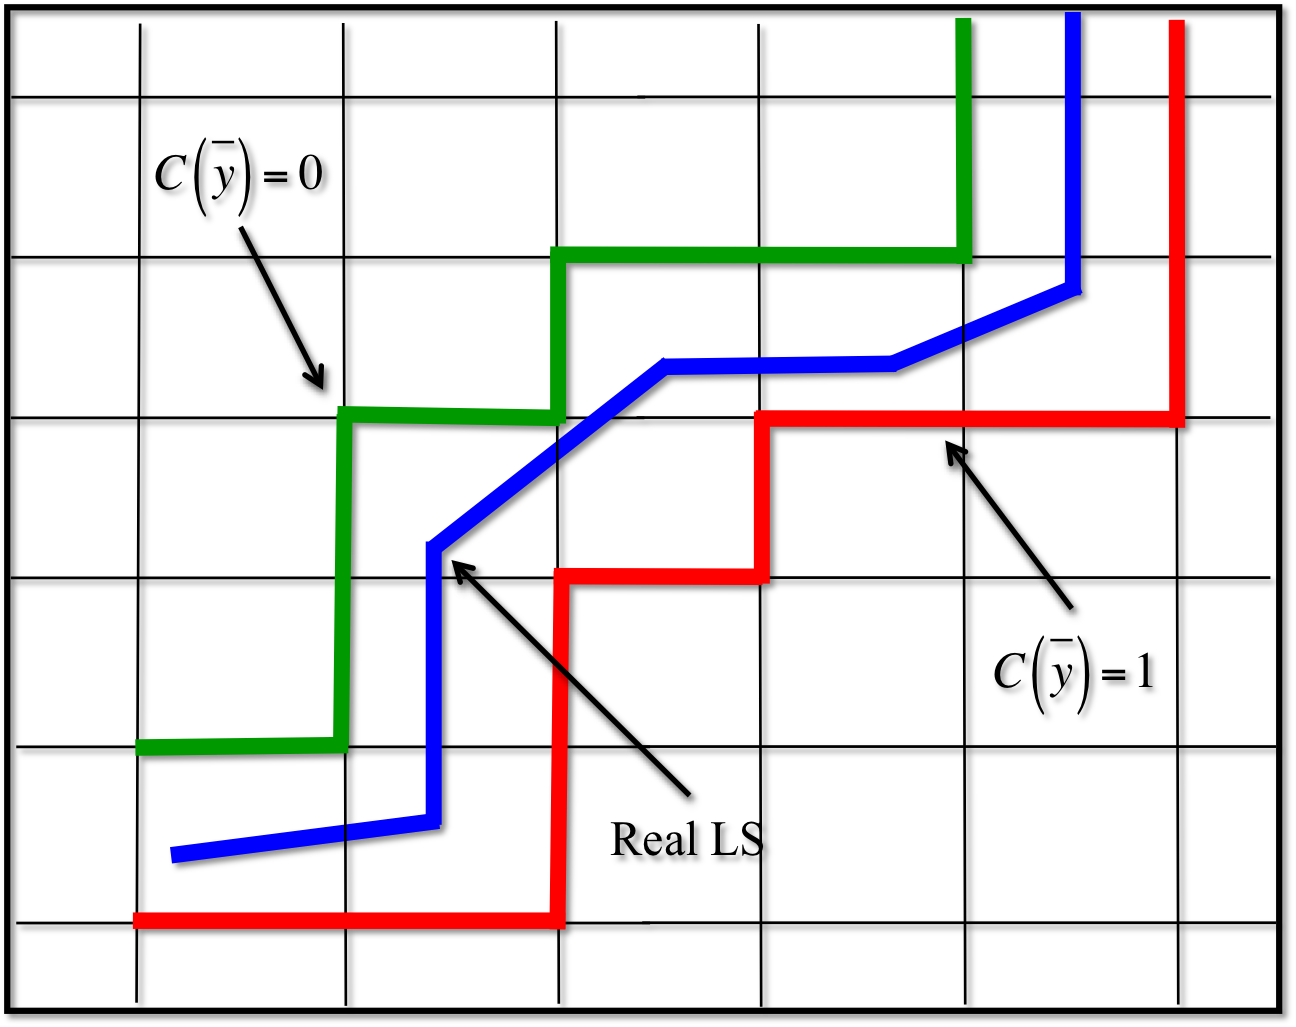
\includegraphics[width=1.0\textwidth]  {pics/LSgoalFunctionExample.png}
  \caption{Example of limit surface search evaluation grid (where $\overline{y}=\overline{\theta}$).}
  \label{fig:LSgoalFunctionExample}
\end{figure}
Each evaluation of the ``goal'' function in one of the grid nodes implies
the evaluation of the high-fidelity code (e.g. system simulator) for the
corresponding set of entries in the uncertain space. As already
mentioned, the evaluation of the high fidelity code is computationally
expensive and, in order to identify the LS, one should appraise
each point in the N-D grid covering the uncertainty space.
Discretization depends on the accuracy requested by the user. In
most cases, this approach is not feasible and, consequentially, the
process needs to be accelerated using ``predicting'' methods that are
represented by the employment of supervised learning algorithms
(i.e., ROMs).

This approach is commonly referred to as an active learning process
that ultimately results in training of a ROM of type classifier capable of
predicting the outcome of the ``goal'' function for any given point of
the uncertain space.
In an active learning process, a supervised learning algorithm is
combined with criteria to choose the next node in the N D grid that
needs explored, using the high fidelity physical model. This process is
repeated until, under a particular metric, the prediction capabilities of
the supervised learning algorithm do not improve by further increasing
the training set.

In more detail, the iterative scheme could be summarized through the following steps:
\begin{enumerate}
  \item A limited number of points in the uncertain space $\left \{
  \overline{x}_{k} \right \}$ are selected via one of the forward
  sampling strategies (e.g., stratified or Monte Carlo)
  \item The high fidelity code is used to compute the status of the
  system for the set of points in the input set:
  $
  \left \{ \overline{\theta}(t)\right \}_{k} = H\left ( \left \{ \overline{x} \right
  \}_{k},t \right )
  $.
  \item The ``goal'' function is evaluated at the phase space coordinate
  of the system:
  $\left \{ c \right \}_{k} = C\left ( \left \{ \overline{\theta}(t)\right \}_{k}
  \right )$
   \item The set of pairs $\left \{ \left ( \overline{x},c \right )_{k} \right \}$
   are used to train a ROM of type classifier, $G\left ( \left \{
   \overline{x}_{k} \right \} \right )$
   \item The ROM classifier is used to predict the values of the ``goal''
   function for all the $N$ nodes of the N-D grid in the domain space:
   \begin{equation}
   \left (G\left ( \left \{ \overline{x} \right \}_{j} \right ) \sim \left \{ c \right
   \}_{j}, j=1,...,N  \right )
    \end{equation}
    \item The values of the ``goal''  function are used to determine the
    LS location based on the change of values of  $\left \{ c \right
    \}_{j}$:
    \begin{equation}
    \left \{ c \right \}_{j}\rightarrow \partial V_{F}
     \end{equation}
     \item A new point is chosen to increase the training set and a new
     pair is generated
     \item The procedure is repeated starting from Step 3 until
     convergence is achieved. The convergence is achieved when
     there are no changes in the location of the LS after a certain
     number of consecutive iterations.
\end{enumerate}
The iteration scheme is graphically shown in
Figure~\ref{fig:LimitSurfaceAlgoFlow}.
\begin{figure}[h!]
  \centering
  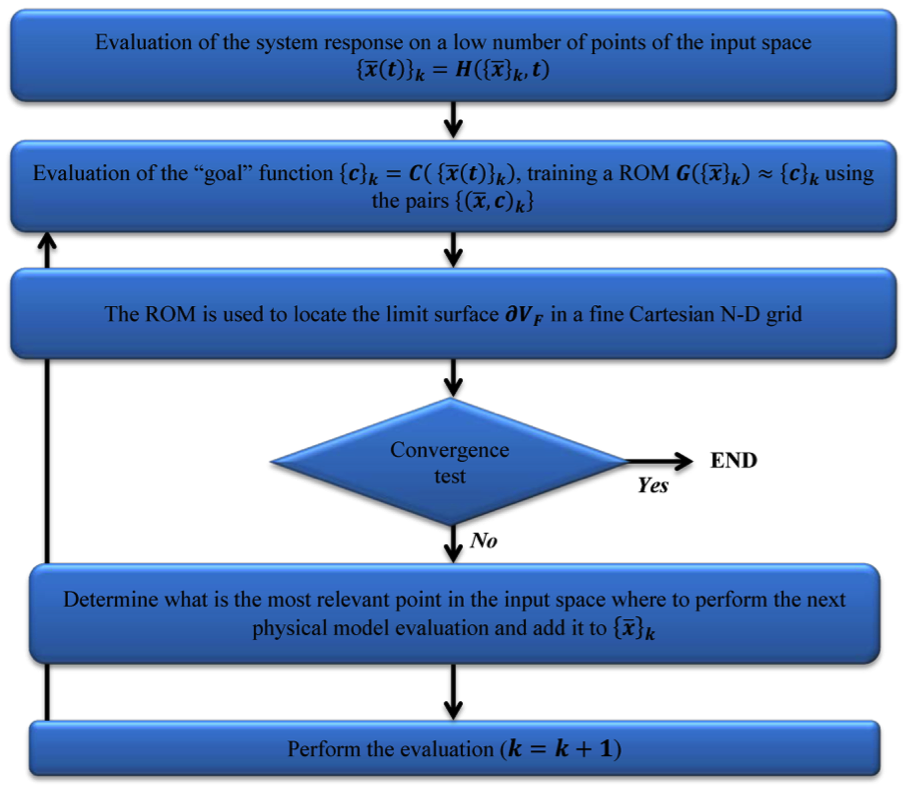
\includegraphics[width=1.0\textwidth]  {pics/LimitSurfaceAlgoFlow.png}
  \caption{Limit surface search algorithm conceptual scheme.}
  \label{fig:LimitSurfaceAlgoFlow}
\end{figure}
Note that there is an additional requirement
regarding the LS search algorithm:the LS location
has to stay constant for a certain number (user defined) of consecutive
iterations. The reason for this choice is determined by the attempt to
mitigate the effect of the build of non-linear bias in the searching
pattern. Indeed, the searching algorithm might focus too much on a
certain region of the LS while putting too few points in other zones
and completely hiding undiscovered topological features of the LS.
Regarding the strategy to choose the nodes on the N-D grid that
needs evaluated in the iterative process for the LS identification, it has
been decided to employ a metric based on the
distance between the predicted LS and the evaluations already
performed. The points on the LS are ranked based on the distance
from the closest training point already explored (the larger is the
distance the higher is the score for the candidate point), and based on
its persistence (the larger is the number of time the prediction of the
``goal'' function for that point have changed the higher is the score).
Since this approach creates a queue of ranked candidates, it could be
used also in the parallel implementation of the algorithm. When
several training points are run in parallel, it is possible that the
evaluation of one additional point does not alter dramatically the
location of the LS. Consequently, it is possible that the candidate with
the highest score is already being submitted for evaluation and
possibly the simulation is not yet completed. In this case, to avoid
submitting the same evaluation point twice, the algorithm searches
among all the ranked candidates (in descending order) for the one
that was not submitted for evaluation. Even if it is extremely unlikely
that all the candidates were submitted, in this remote event, the
method will choose the next point employing a Monte Carlo strategy.
%%%%%%%%%
%%%%%%%%% Acceleration through Multi-grid Approach
%%%%%%%%%
\paragraph{Acceleration through Multi-grid Approach}
\label{par:LSaccelerationMultiGrid}
The location of the LS, being a numerical iterative process, can be
known given a certain tolerance. As already mentioned, the LS search
is done by constructing an evaluation grid on which the acceleration
ROM is inquired. The tolerance of the iterative process determines how
the evaluation grid is discretized. Before addressing the acceleration
scheme, it is important
to introduce some concepts on the employed numerical process.
\begin{figure}[h!]
  \centering
  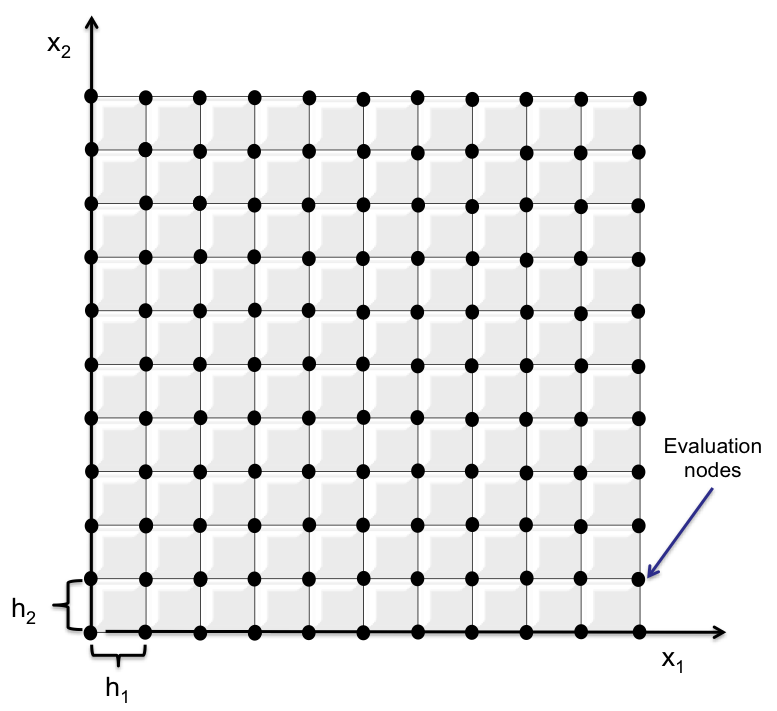
\includegraphics[width=1.0\textwidth]  {pics/DiscretizationGrid.png}
  \caption{Discretization grid.}
  \label{fig:DiscretizationGrid}
\end{figure}
\\Assume that each of $D$ dimensions of the uncertain domain is
discretized with the same number of equally-spaced nodes $N$ (see
Figure~\ref{fig:DiscretizationGrid}), with discretization size indicated
by $h_{i}$. Hence, the Cartesian grid contains $N^{D}$ individual
nodes, indexed through the multi-index vector $\overline{j} = \left (
j_{i=1\rightarrow D} \right ), j_{i} \leq N \forall i$. Introducing the
vectors  $\overline{I} = (1, ..., 1)$ and
$\overline{N} = (N, ..., N)$, the ``goal'' function is expressed on this N-
D grid as:
\begin{equation}
C\left ( \overline{x} \right ) =
\mathlarger{\sum}_{\overline{j}=\overline{I}}^{\overline{N}} \varphi_{\overline{j}}\left
( \overline{x} \right ) C\left ( \overline{x}_{\overline{j}} \right )
\end{equation}
where $\varphi_{\overline{j}}$ is the characteristic function of the hyper-volume $\Omega_{\overline{j}}$ surrounding the node
 $\overline{x}_{\overline{j}}$:
 \begin{equation}
 \varphi_{\overline{j}}\left ( \overline{x} \right ) =
\left\{\begin{matrix}
1 & if \: \overline{x} \in \Omega_{\overline{j}} \\
0 & if \: \overline{x} \notin \Omega_{\overline{j}}
\end{matrix}\right.
\end{equation}
where:
 \begin{equation}
 \label{eq:OmegaEq}
 \Omega_{\overline{j}} = \prod_{i=1}^{D}\left [ x_{j_{i}} - \frac{h_{i}}{2},
 x_{j_{i}} + \frac{h_{i}}{2}  \right ]
 \end{equation}
 The probability of the uncertain parameters is expressed as:
 \begin{equation}
 pdf_{\overline{X}}\left ( \overline{x} \right ) =
\mathlarger{\sum}_{\overline{j}=\overline{I}}^{\overline{N}}
\varphi_{\overline{j}}\left ( \overline{x} \right )
pdf_{\overline{X}}\left ( \overline{x}_{\overline{j}} \right )
 \end{equation}
Following the approach briefly explained in Section
\ref{sec:LSconcept}, the probability of the event (e.g., failure) could be
expressed as:
 \begin{equation}
 \label{eq:Pf}
  P_{F}=\left ( \prod_{i=1}^{D}h_{i} \right )
  \mathlarger{\sum}_{\overline{j}=
  \overline{I}}^{\overline{N}}pdf_{\overline{X}}\left (
  \overline{x_{\overline{j}}} \right )
  C\left ( \overline{x}_{\overline{j}} \right )
 \end{equation}
Under certain assumptions, the concept of active hyper-volume
$V_{A}$ as the region of the input space identified by the support of
the uncertain parameters’ probability density functions
$pdf_{\overline{X}}\left ( \overline{x} \right )$ could be introduced;
Equation ~\ref{eq:Pf} is recast, using a Taylor expansion, as follows:
 \begin{equation}
P_{F}= \bigintssss_{V} C\left ( \overline{x} \right )\: pdf_{\overline{X}}\left (
\overline{x}  \right )\: d\overline{x} =\bigintssss_{V_{A}}C\left ( \overline{x}
\right )\:
\left [
\mathlarger{\sum}_{\overline{j}=\overline{I}}^{\overline{N}}\varphi_{\overline{j}}\left (
\overline{x} \right )
\left ( pdf_{\overline{X}}\left ( \overline{x}_{\overline{j}} \right ) +
\mathlarger{\sum}_{i=1}^{D} \frac{\partial pdf_{\overline{X}}}{\partial x_{i}}|
_{\overline{x}_{\overline{j}}} \: \left ( x_{i} - x_{j_{i}} \right ) \right ) \right
] d\overline{x}
 \end{equation}
And, considering the evaluation grid as:
\begin{equation}
\label{eq:PfEq}
P_{F}= \mathlarger{\sum}_{\begin{matrix}
\overline{j}=\overline{I} \\ \overline{x}_{\overline{j}} \in V_{A} \end{matrix}}^{\overline{N}}
\bigintssss_{\overline{x}_{\overline{j}} - \overline{h}/2}^{\overline{x}_{\overline{j}} + \overline{h}/2} C\left ( \overline{x} \right )\:
\left [  \mathlarger{\sum}_{\overline{j}=\overline{I}}^{\overline{N}}\varphi_{\overline{j}}\left ( \overline{x} \right )
\left ( pdf_{\overline{X}}\left ( \overline{x}_{\overline{j}} \right ) +
\mathlarger{\sum}_{i=1}^{D} \frac{\partial pdf_{\overline{X}}}{\partial x_{i}}|_{\overline{x}_{\overline{j}}} \: \left ( x_{i} - x_{j_{i}} \right ) \right ) \right ] d\overline{x}
\end{equation}
At this point, it is possible to label, in the active hyper-volume, the sub-
domain identified by the nodes where the ``goal'' function
$C(\overline{x})$ changes its value (the frontier nodes between the
region where $C(\overline{x})=1$ and $C(\overline{x})=0$) $V_{A} \cap
V_{\partial V_{F}}$.
\\ Consequentially, it is possible to identify the sub-domains in which the  ``goal''  function $C(\overline{x})$ is equal to $0$ ($V_{A} \cap V_{\partial V_{C(\overline{x})=0}} \notin V_{A} \cap V_{\partial V_{F}}$):

\begin{equation}
\mathlarger{\sum}_{\begin{matrix}
\overline{j}=\overline{I} \\ \overline{x}_{\overline{j}} \in V_{A} \cap V_{C(\overline{x})=0} \end{matrix}}^{\overline{N}}
\bigintssss_{\overline{x}_{\overline{j}} - \overline{h}/2}^{\overline{x}_{\overline{j}} + \overline{h}/2} C\left ( \overline{x} \right )\:
\left ( pdf_{\overline{X}}\left ( \overline{x}_{\overline{j}} \right ) +
\mathlarger{\sum}_{i=1}^{D} \frac{\partial pdf_{\overline{X}}}{\partial x_{i}}|_{\overline{x}_{\overline{j}}} \: \left ( x_{i} - x_{j_{i}} \right ) \right )   d\overline{x}
\end{equation}
in which the  ``goal''  function $C(\overline{x})$ is equal to $1$ ($V_{A} \cap V_{\partial V_{C(\overline{x})=1}} \notin V_{A} \cap V_{\partial V_{F}}$):
\begin{equation}
\begin{matrix}
\mathlarger{\sum}_{\begin{matrix}
\overline{j}=\overline{I} \\ \overline{x}_{\overline{j}} \in V_{A} \cap V_{C(\overline{x})=1} \end{matrix}}^{\overline{N}}
\bigintssss_{\overline{x}_{\overline{j}} - \overline{h}/2}^{\overline{x}_{\overline{j}} + \overline{h}/2} C\left ( \overline{x} \right )\:
\left ( pdf_{\overline{X}}\left ( \overline{x}_{\overline{j}} \right ) +
\mathlarger{\sum}_{i=1}^{D} \frac{\partial pdf_{\overline{X}}}{\partial x_{i}}|_{\overline{x}_{\overline{j}}} \: \left ( x_{i} - x_{j_{i}} \right ) \right )   d\overline{x} =
\\
= \mathlarger{\sum}_{\begin{matrix}
\overline{j}=\overline{I} \\ \overline{x}_{\overline{j}} \in V_{A} \cap V_{C(\overline{x})=1} \end{matrix}}^{\overline{N}}
\bigintssss_{\overline{x}_{\overline{j}} - \overline{h}/2}^{\overline{x}_{\overline{j}} + \overline{h}/2}
\left ( pdf_{\overline{X}}\left ( \overline{x}_{\overline{j}} \right ) +
\mathlarger{\sum}_{i=1}^{D} \frac{\partial pdf_{\overline{X}}}{\partial x_{i}}|_{\overline{x}_{\overline{j}}} \: \left ( x_{i} - x_{j_{i}} \right ) \right )   d\overline{x}
\end{matrix}
\end{equation}
Equation ~\ref{eq:PfEq} is now expressed as:
 \begin{equation}
 \label{eq:PfEqFinal}
 \begin{matrix}
P_{F} = \mathlarger{\sum}_{\begin{matrix}
\overline{j}=\overline{I} \\ \overline{x}_{\overline{j}} \in V_{A} \cap
V_{C(\overline{x})=1} \end{matrix}}^{\overline{N}}
\left ( \prod_{i=1}^{D}
 h_{i} \right )
\: pdf_{\overline{X}} ( \overline{x}_{\overline{j}}) + O(h^{N+1}) +
 \\
 + \mathlarger{\sum}_{\begin{matrix}
\overline{j}=\overline{I} \\ \overline{x}_{\overline{j}} \in V_{A} \cap
V_{\partial V_{f}} \end{matrix}}^{\overline{N}}
\bigintssss_{\overline{x}_{\overline{j}} -
\overline{h}/2}^{\overline{x}_{\overline{j}} + \overline{h}/2} C\left (
\overline{x} \right )\: \left ( pdf_{\overline{X}}\left (
\overline{x}_{\overline{j}} \right ) +
\mathlarger{\sum}_{i=1}^{D} \frac{\partial pdf_{\overline{X}}}{\partial
x_{i}}|_{\overline{x}_{\overline{j}}} \: \left ( x_{i} - x_{j_{i}} \right ) \right )
d\overline{x}
\end{matrix}
 \end{equation}
As inferred from Equation ~\ref{eq:PfEqFinal}, the process is bounded if the
surface area-to-volume ratio (amount of surface area per unit volume) is
in favor of the volume:
\begin{equation}
\label{eq:convergenceCondition}
\mathlarger{\sum}_{\begin{matrix}
\overline{j}=\overline{I} \\ \overline{x}_{\overline{j}} \in V_{A} \cap
V_{C(\overline{x})=1} \end{matrix}}^{\overline{N}}
\left ( \prod_{i=1}^{D}
 h_{i} \right )
\: pdf_{\overline{X}} ( \overline{x}_{\overline{j}})
\gg
\sum_{\begin{matrix}
\overline{j}=\overline{I} \\ \overline{x}_{\overline{j}} \in V_{A} \cap
V_{\partial V_{f}} \end{matrix}}^{\overline{N}}
\left | \int_{\overline{x}_{\overline{j}} -
\overline{h}/2}^{\overline{x}_{\overline{j}} + \overline{h}/2}   pdf_{\overline{X}}\left (
\overline{x}_{\overline{j}} \right )  \right |
d\overline{x}
\end{equation}
If the grid is built in the transformed space of probability (i.e., replacing the measure $d\overline{x}$ with $d \overline{\mu }\: \: pdf_{\overline{X}}\left ( \overline{x}_{\overline{j}} \right )$ the condition expressed in Equation ~\ref{eq:convergenceCondition} is reduced:
\begin{equation}
number \: \:  nodes \in V_{A} \cap V_{C(\overline{x})=1} \gg number \: \:  nodes  \in V_{A} \cap V_{\partial V_{F}}
\end{equation}
This means that error is bounded by the total probability contained in the cells on the frontier of the LS.

Based on this derivation, it is clear how important it is to keep the
content of the total probability on the frontier of the LS as low as
possible, and simultaneously, increase the importance of the volume of
the failure/event region as much as possible (to improve the surface
area-to-volume ratio).

To do that, the step size in probability should be significantly
reduced ( $h_{i}^{p} \rightarrow 0^{+}$). Even if this is theoretically
feasible, it is computational inapplicable. To approach a similar result, it
is possible to learn from other numerical methods that use the
technique of adaptive meshing for the resolution of the partial
differential equation system (e.g., finite element methods).

For this reason, an acceleration scheme was designed and developed
employing a multi-grid approach. The main idea, it is to recast the
iterative process in two different sub-sequential steps. Firstly,
performing the LS search on a coarse evaluation grid, and once
converged, adaptively refining the cells that lie on the frontier of the LS
($V_{A} \cap V_{\partial V_{F}}$) and, consequentially, converging on
the new refined grid.
\\The iteration scheme is graphically shown in
Figure~\ref{fig:LimitSurfaceMultiGridAlgoFlow}.
\begin{figure}[h!]
  \centering
  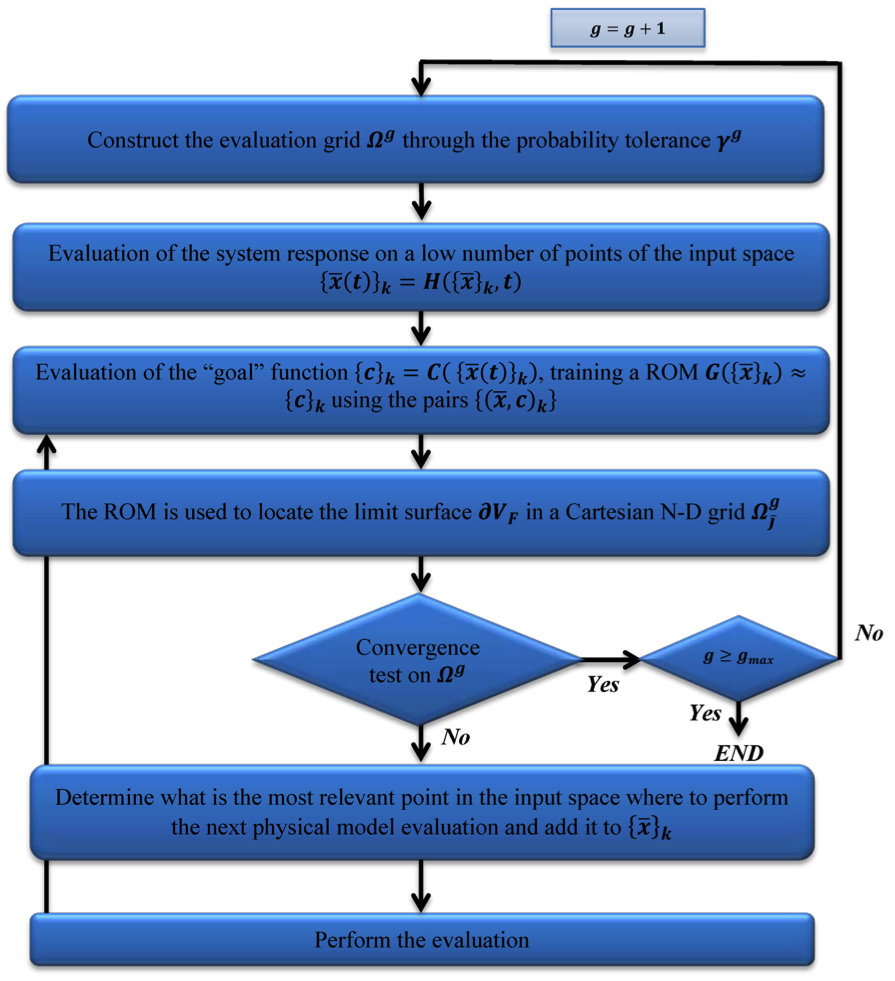
\includegraphics[width=1.0\textwidth]  {pics/LimitSurfaceMultiGridAlgoFlow.png}
  \caption{Multi-grid limit surface search scheme.}
  \label{fig:LimitSurfaceMultiGridAlgoFlow}
\end{figure}
In more detail, the iterative scheme could be summarized through the
following steps:
\begin{enumerate}
  \item The user specifies two tolerances in probability $(CDF):
  \gamma^{g=1}$ for the initial coarse grid and $\gamma^{g=2}$
  for the refined grid, where  $ \gamma^{g=1} >  \gamma^{g=2}$;
  \item Following Equation ~\ref{eq:OmegaEq}, the initial coarse evaluation
  grid $\Omega^{1}$ is constructed ($N^{g=1}$ total nodes). The
  discretization of this grid is done to have cells with a content of
  probability equal to $\gamma^{g=1}$.
  \item A limited number of points in the uncertain space $\left \{
  \overline{x}_{k} \right \}$ are selected via one of the forward
  sampling strategies (e.g., stratified or Monte Carlo).
  \item The high fidelity code is used to compute the status of the
  system for the set of points in the input set:
  $
  \left \{ \overline{\theta}(t)\right \}_{k} = H\left ( \left \{ \overline{x} \right
  \}_{k},t \right )
  $.
  \item The ``goal'' function is evaluated at the phase space coordinate
  of the system:
  $\left \{ c \right \}_{k} = C\left ( \left \{ \overline{\theta}(t)\right \}_{k}
  \right )$.
   \item The set of pairs $\left \{ \left ( \overline{x},c \right )_{k} \right \}$
   are used to train a ROM of type classifier, $G\left ( \left \{
   \overline{x}_{k} \right \} \right )$.
   \item The ROM classifier is used to predict the values of the ``goal''
   function for all the $N^{g=1}$ nodes of the N-D grid in the domain
   space:
   \begin{equation}
   \left (G\left ( \left \{ \overline{x} \right \}_{j} \right ) \sim \left \{ c \right
   \}_{j}, j=1,...,N^{g=1}  \right )
    \end{equation}
    \item The values of the ``goal''  function are used to determine the
    LS location based on the change of values of  $\left \{ c \right
    \}_{j}$:
    \begin{equation}
    \left \{ c \right \}_{j}\rightarrow \partial V_{F}
     \end{equation}
     \item A new point is chosen to increase the training set and a new
     pair is generated.
     \item The procedure is repeated starting from Step 5 until
     convergence is achieved on grid $\Omega^{g}$.The convergence
     is reached when there are no changes in the location of the LS
     after a certain number of consecutive iterations (user defined).
     \item When the convergence is achieved on the coarse grid
     $\Omega^{g=1}$, all the cells that lie on the frontier of the LS
     ($V_{A} \cap V_{\partial V_{F}}$) are refined to contain an amount of
     probability equal to  $\gamma^{g=2}$.
     \item Steps 7 through 9 are performed based on the new refined
     grid. Finally, the process starts again by performing Steps 5
     through 10, until the convergence is achieved in the refined grid.
\end{enumerate}
As shown in Figure~\ref{fig:LimitSurfaceMultiGridAlgoFlow}, the
algorithm consists in searching the location of the LS proceeding with
subsequential refinement of the sub-domain, in the active space, that
contains the LS. In this way, the computational burden is kept as low as
possible. In addition, another advantage of this approach is that, since
the refinement grid represents a constrained domain, the sub-
sequential ROM training process can be regularized, since the LS
between an iteration and the other can move, at maximum, within the
refinement domain.

%%%%%%%%%%%%%%%%
\subsubsection{Limit Surface Search sampling through RAVEN}
\label{subsub:LSsamplingExample}
The goal of this Section is to learn how to:
 \begin{enumerate}
   \item Set up a LS Search sampling for efficiently perturb a driven code
   \item Use the LS Integral Post-processor for computing the probability of failure of the system subject to the same
   ``goal'' function
   \item Plot the obtained LS.
\end{enumerate}
In order to accomplish these tasks, the following RAVEN \textbf{Entities} (XML blocks in the input files) are defined:
\begin{enumerate}
   \item \textbf{\textit{RunInfo}}:
\begin{lstlisting}[style=XML,morekeywords={arg,extension,pauseAtEnd,overwrite}]
  <RunInfo>
    <JobName>LSsearch</JobName>
    <Sequence>
      sample,computeLSintegral,writeHistories
    </Sequence>
    <WorkingDir>LSsearch</WorkingDir>
    <batchSize>8</batchSize>
  </RunInfo>
\end{lstlisting}
   As shown in Section~\ref{sub:EntitiesAndFlow}, the \textit{RunInfo} \textbf{Entity} is intended to set up the analysis
   that the user wants to perform. In this specific case, three steps (\xmlNode{Sequence}) are  sequentially run
   using eight processors (\xmlNode{batchSize}).
   \item \textbf{\textit{Files}}:
\begin{lstlisting}[style=XML,morekeywords={arg,extension,pauseAtEnd,overwrite}]
  <Files>
    <Input name="referenceInput.xml" type="input">referenceInput.xml</Input>
    <Input name="LSintegral.csv" type="">LSintegral.csv</Input>
  </Files>
\end{lstlisting}
   Since the driven code uses a single input file, in this Section the original input is placed. As detailed in the user manual
   the attribute  \xmlAttr{name} represents the alias that is going to be
   used in all the other input blocks in order to refer to this file.
   \\In addition the output file used in \xmlNode{Sequence}
   \textit{computeLSintegral} is here inputted.
   \item \textbf{\textit{Models}}:
\begin{lstlisting}[style=XML,morekeywords={arg,extension,pauseAtEnd,overwrite}]
  <Models>
    <Code name="testModel" subType="GenericCode">
      <executable>
      ../physicalCode/analyticalbateman/AnalyticalDplMain.py
      </executable>
      <clargs arg="python" type="prepend"/>
      <clargs arg="" extension=".xml" type="input"/>
      <clargs arg="" extension=".csv" type="output"/>
      <prepend>python</prepend>
    </Code>
    <ROM name="AccelerationROM" subType="SciKitLearn">
      <Features>sigma-A,decay-A</Features>
      <Target>goalFunction</Target>
      <SKLtype>neighbors|KNeighborsClassifier</SKLtype>
      <n_neighbors>1</n_neighbors>
    </ROM>
    <PostProcessor name="integralLS" subType="LimitSurfaceIntegral">
      <tolerance>0.001</tolerance>
      <integralType>MonteCarlo</integralType>
      <seed>20021986</seed>
      <target>goalFunction</target>
      <variable name="sigma-A">
        <distribution>sigmaA</distribution>
      </variable>
      <variable name="decay-A">
        <distribution>decayConstantA</distribution>
      </variable>
    </PostProcessor>
  </Models>
\end{lstlisting}
 As mentioned above, the goal of this example is the employment of
 an efficient sampling strategy, having as goal the determination of the
 failure of a system.

 In addition to the previously explained Code
 model,
 the ROM of type \textit{SciKitLearn} is here specified. The ROM will be
 used in the adaptive sampling strategy \textit{LimitSurfaceSearch} in
 order to accelerate the convergence of the method. As it can be seen,
 a nearest neighbor classifier is used, targeting only two uncertainties
 $sigma-A and decay-A$.
 \\ For the computation of the probability of failure (see the following), a
 Post-Processor (PP) of type \textit{LimitSurfaceIntegral} is here
 specified.This PP performs an integral of the LS
 generated by the adaptive sampling technique.
   \item \textbf{\textit{Distributions}}:
\begin{lstlisting}[style=XML]
  <Distributions>
      <Uniform name="sigmaA">
          <lowerBound>0</lowerBound>
          <upperBound>1000</upperBound>
      </Uniform>
      <Uniform name="decayConstantA">
          <lowerBound>0.00000001</lowerBound>
          <upperBound>0.0000001</upperBound>
      </Uniform>
  </Distributions>
\end{lstlisting}
  In the Distributions XML Section, the stochastic model for the
  uncertainties  treated by the LS search sampling are reported. In
  this case two distributions are defined:
  \begin{itemize}
    \item $sigmaA \sim \mathbb{U}(0,1000)$, used to model the uncertainty
    associated with  the Model \textit{sigma-A}
    \item  $decayConstantA \sim \mathbb{U}(1e-8,1e-7)$,  used to
    model the uncertainty
    associated with  the Model \textit{decay-A}.
  \end{itemize}
   \item \textbf{\textit{Samplers}}:
\begin{lstlisting}[style=XML,morekeywords={arg,extension,pauseAtEnd,overwrite}]
  <Samplers>
    <LimitSurfaceSearch name="LSsearchSampler">
      <ROM              class="Models"      type="ROM">AccelerationROM</ROM>
      <Function         class="Functions"   type="External">goalFunction</Function>
      <TargetEvaluation class="DataObjects" type="PointSet">samples</TargetEvaluation>
      <Convergence forceIteration="False" limit="50000" persistence="20"  weight="CDF">0.00001</Convergence>
      <variable name="sigma-A">
        <distribution>sigmaA</distribution>
      </variable>
      <variable name="decay-A">
        <distribution>decayConstantA</distribution>
      </variable>
    </LimitSurfaceSearch>
  </Samplers>
\end{lstlisting}
  In order to employ the LS search sampling strategy, a
  \xmlNode{LimitSurfaceSearch} node needs to be inputted.
  As it can be
  seen from above, each variable is associated to a different distribution
  defined in the  \xmlNode{Distributions} block.
  In addition, the \textit{AccelerationROM}  \xmlNode{ROM} is inputted.
  As already mentioned, this ROM (of type classifier) is used to
  accelerate the convergence of the LS Search method.
  In addition, the goal function \textit{goalFunction}  and the
  \textit{samples} are here reported.
  \\For this example, a convergence criterion of $1.0e-5$ is set. To reach such a confidence with a Monte-Carlo, millions of
  samples would be needed.
   \item \textbf{\textit{Functions}}:
\begin{lstlisting}[style=XML,morekeywords={arg,extension,pauseAtEnd,overwrite}]
 <Functions>
   <External file="goalFunction" name="goalFunction">
     <variable>A</variable>
   </External>
 </Functions>
\end{lstlisting}
 As already mentioned, the LS search sampling strategy uses
 a goal function in order to identify the regions of the uncertain space
 that are more informative. The \textit{goalFunction} used for this
 example is reported below. As it can be seen, if the final response $A$
 is $<=$ of $0.3$ , the system is considered to be in a ``safe'' condition.
\begin{lstlisting}[language=python]
def __residuumSign(self):
  returnValue = 1.0
  if self.A  <= 0.3:
    returnValue = -1.0
  return returnValue
\end{lstlisting}

   \item \textbf{\textit{DataObjects}}:
\begin{lstlisting}[style=XML,morekeywords={arg,extension,pauseAtEnd,overwrite}]
  <DataObjects>
    <PointSet name="limitSurface">
      <Input>sigma-A,decay-A</Input>
      <Output>goalFunction</Output>
    </PointSet>
    <PointSet name="samples">
      <Input>sigma-A,decay-A</Input>
      <Output>A,B,C,D,time</Output>
    </PointSet>
    <HistorySet name="histories">
      <Input>sigma-A,decay-A</Input>
      <Output>A,B,C,D,time</Output>
    </HistorySet>
  </DataObjects>
\end{lstlisting}
  In this block, three \textit{DataObjects} are defined: 1) PointSet
  named ``samples'' used to collect the final outcomes of the code, 2)
  HistorySet named ``histories'' in which the full time responses of the
  variables $A,B,C,D$ are going to be stored, 3) PointSet named
  ``limitSurface'' used  to export the LS location (in the uncertain space) during the employment of the sampling strategy.
 %%%%%%%%%%%%%%%%%%%%%%%%%%%%%%%%%%%%%%%%%%%%%%%%%%%%%%%%%%
 %%%%%%%%%%%%%%%%%%%%%%%%%%%%%%%%%%%%%%%%%%%%%%%%%%%%%%%%%%
 %figure samples
 \begin{figure}[h!]
  \centering
  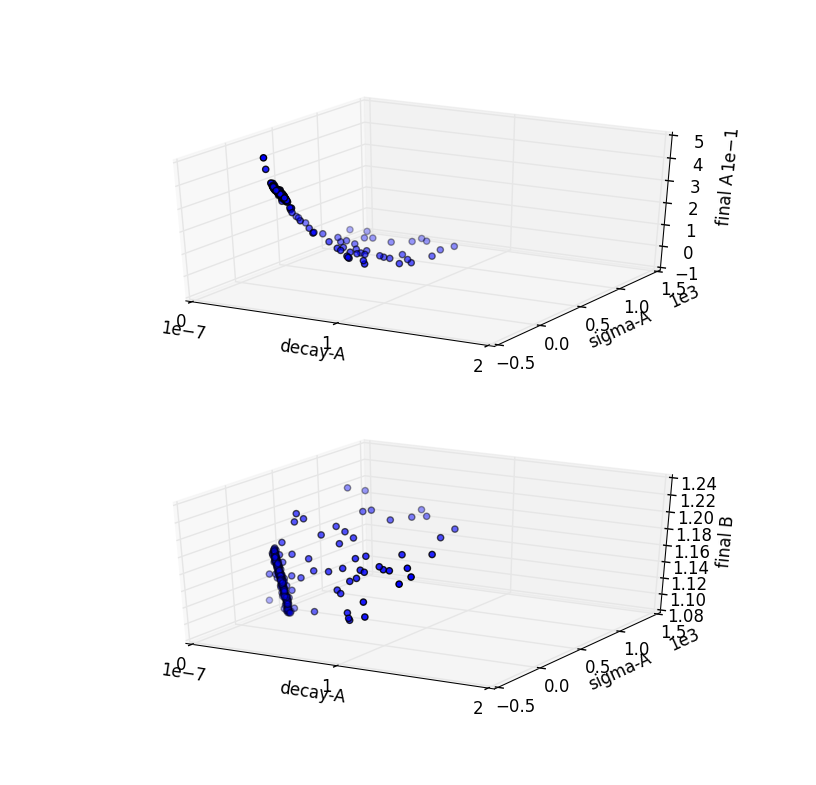
\includegraphics[scale=0.7]{pics/LS_pointsets.png}
  \caption{Plot of the samples generated by the LS search sampling for variables $A,B$.}
  \label{fig:LS_pointsets}
 \end{figure}
 %%%%%%%%%%%%%%%%%%%%%%%%%%%%%%%%%%%%%%%%%%%%%%%%%%%%%%%%%%
 %%%%%%%%%%%%%%%%%%%%%%%%%%%%%%%%%%%%%%%%%%%%%%%%%%%%%%%%%%
   \item \textbf{\textit{Steps}}:
\begin{lstlisting}[style=XML,morekeywords={arg,extension,pauseAtEnd,overwrite}]
  <Steps>
    <MultiRun name="sample">
      <Input          class="Files"       type="input">referenceInput.xml</Input>
      <Model          class="Models"      type="Code">testModel</Model>
      <Sampler        class="Samplers"    type="LimitSurfaceSearch">LSsearchSampler</Sampler>
      <SolutionExport class="DataObjects" type="PointSet">limitSurface</SolutionExport>
      <Output         class="DataObjects" type="PointSet">samples</Output>
      <Output         class="DataObjects" type="HistorySet">histories</Output>
    </MultiRun>
    <PostProcess name="computeLSintegral">
      <Input  class="DataObjects" type="PointSet"     >limitSurface</Input>
      <Model  class="Models"      type="PostProcessor">integralLS</Model>
      <Output class="DataObjects" type="PointSet"     >limitSurface</Output>
      <Output class="Files"       type=""             >LSintegral.csv</Output>
    </PostProcess>
    <IOStep name="writeHistories" pauseAtEnd="True">
      <Input  class="DataObjects"      type="HistorySet">histories</Input>
      <Input  class="DataObjects"      type="PointSet">samples</Input>
      <Input  class="DataObjects"      type="PointSet">limitSurface</Input>
      <Output class="OutStreamManager" type="Plot">samplesPlot3D</Output>
      <Output class="OutStreamManager" type="Plot">historyPlot</Output>
      <Output class="OutStreamManager" type="Print">samples</Output>
      <Output class="OutStreamManager" type="Plot">limitSurfacePlot</Output>
      <Output class="OutStreamManager" type="Print">histories</Output>
    </IOStep>
  </Steps>
\end{lstlisting}
  %%%%%%%%%%%%%%%%%%%%%%%%%%%%%%%%%%%%%%%%%%%%%%%%%%%%%%%%%%
 %figure samples
 \begin{figure}[h!]
  \centering
  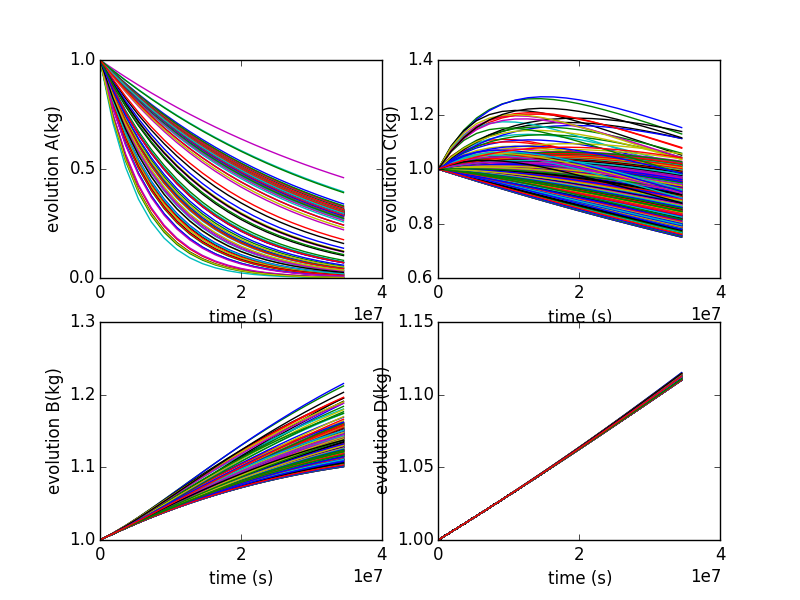
\includegraphics[scale=0.7]{pics/LS_histories.png}
  \caption{Plot of the histories generated by the LS search method for variables $A,B,C,D$.}
  \label{fig:LS_histories}
 \end{figure}
 %%%%%%%%%%%%%%%%%%%%%%%%%%%%%%%%%%%%%%%%%%%%%%%%%%%%%%%%%%
   Finally, all the previously defined \textbf{Entities} can be combined in
   the \xmlNode{Steps} block. As inferable,
   three \xmlNode{Steps} have been inputted:
   \begin{itemize}
     \item \xmlNode{MultiRun} named ``sample'', used to run the multiple
     instances of the driven code and
     collect the outputs in the two \textit{DataObjects}. As it can be
     seen, the \xmlNode{Sampler} is inputted to communicate to the
     \textit{Step} that the driven code needs to
     be perturbed through the LS search sampling strategy;
     \item \xmlNode{PostProcess} named ``computeLSintegral'', used to
     compute the probability of failure of the system based on the LS generated employing the LS search strategy. This
     probability is computed integrating the LS with a Monte-Carlo
     method.
     \item  \xmlNode{IOStep} named ``writeHistories'', used to 1) export
     the ``histories'' and ``samples''  \textit{DataObjects}
     \textbf{Entity} in a CSV file and 2) plot the data and the Limit Surface
     in  PNG files and on the screen.
   \end{itemize}
\end{enumerate}
 Figure~\ref{fig:LS_histories}
 shows the evolution of the outputs $A,B,C,D$ under uncertainties.
 Figure~\ref{fig:LS_pointsets} shows the final responses  of $A and B$
 of the sampling employed using the driven code.
 Figure~\ref{fig:LSplot}  shows the limit surface for this particular
 example. Only $367$ samples were needed in order to reach the full
 convergence.
 \\The integration of the LS determines a probability of failure of
 $~3.45e-2$.
  %%%%%%%%%%%%%%%%%%%%%%%%%%%%%%%%%%%%%%%%%%%%%%%%%%%%%%%%%%
 %figure samples
 \begin{figure}[h!]
  \centering
  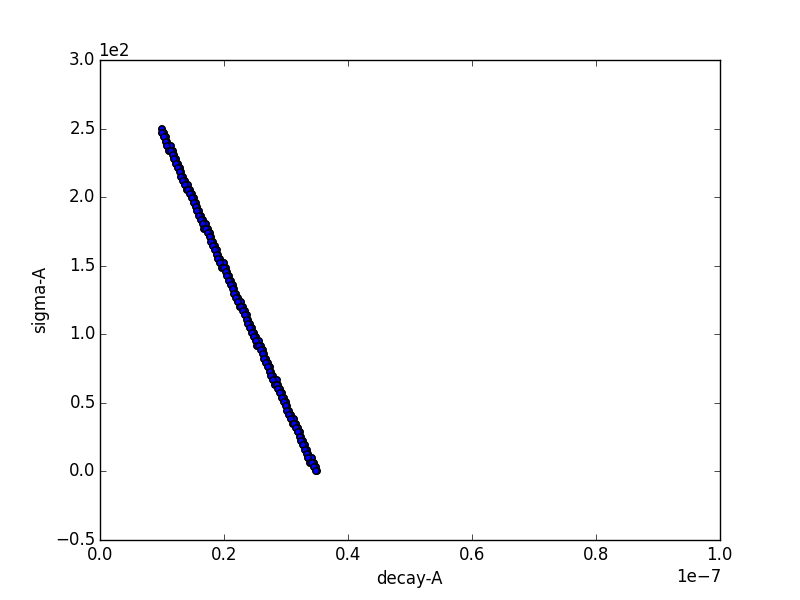
\includegraphics[scale=0.7]{pics/LimitSurfacePlot.png}
  \caption{Limit Surface generated by the LS search method.}
  \label{fig:LSplot}
 \end{figure}
 %%%%%%%%%%%%%%%%%%%%%%%%%%%%%%%%%%%%%%%%%%%%%%%%%%%%%%%%%%









\section{Sampling from Restart}
\label{sec:samplingFromRestart}
In some instances, there are existing solutions stored that are useful to a new sampling calculation.  For
example, if a Monte Carlo run collects 1000 runs, then later the user decides to expand to 1500 runs, the
original 1000 should not be wasted.  In this case, it is desirable to restart sampling.

All \xmlNode{Sampler} entities in RAVEN accept the \xmlNode{Restart} node, which allows the user to provide a
\xmlNode{DataObject} from which sampling can draw.  The way each sampler interacts with this restart data is
dependent on the sampling strategy.

Random sampling strategies, such as the \xmlNode{MonteCarlo} and \xmlNode{Stratified} samplers, increment the
random number generator by the number of samples in the restart data, then continue sampling as normal.

Grid-based sampling strategies, such as \xmlNode{Grid}, \xmlNode{SparseGridCollocation}, and \xmlNode{Sobol},
require specific sampling points.  As each required point in the input space is determined, the sampler will 
check the restart data for a match.  If a match is found, the corresponding output values are used instead of 
sampling the \xmlNode{Model} for that point in the input space.  In order to determine a match, all of the
values in the restart point must be within a relative tolerance of the corresponding point required by the
sampler.  While RAVEN has a default tolerance of 1e-15, the user can adjust this tolerance using the
\xmlNode{restartNode} node in the \xmlNode{Sampler} block.

In order to demonstrate this restart method, we include here an example of restarting a \xmlNode{Grid}
sampler.  This example runs a simple example Python code from the command line using the \xmlNode{GenericCode}
interface.  Within the run the following steps occur:
\begin{enumerate}
  \item A grid is sampled that includes only the endpoints in each dimension.
  \item The results of the first sampling are written to file.
  \item The results in the CSV are read back in to a new \xmlNode{DataObject} called \xmlString{restart}.
  \item A second, more dense grid is sampled that requires the points of the first sampling, plus several
    more.  The results are added both to the original \xmlNode{DataObject} as well as a new one, for
    demonstration purposes.
  \item The results of only the new sampling can be written to CSV because we added the second data object in
    the last step.
  \item Lastly, the complete \xmlNode{DataObject} is written to file, including both the original and more
    dense sampling.
\end{enumerate}
By looking at the contents of \texttt{GRIDdump1.csv}, \texttt{GRIDdump2.csv}, and \texttt{GRIDdump3.csv}, the
progressive construction of the data object becomes clear.  \texttt{GRIDdump1.csv} contains only a few samples
corresponding to the endpoints of the distributions.  \texttt{GRIDdump3.csv} contains all the points necessary
to include the midpoints of the distributions as well as the endpoints.  \texttt{GRIDdump2.csv} contains only
those points that were not already obtained in the first sampling, but still needed for the more dense
sampling.


\footnotesize
\lstinputlisting[style=XML,title=\texttt{raven/tests/framework/Samplers/Restart/Truncated/grid.xml}]
  {../../tests/framework/Samplers/Restart/Truncated/grid.xml}
\normalsize


\section{Reduced Order Modeling}
\label{sec:ROMs}
The development of high-fidelity codes, for thermal-hydraulic systems
and integrated multi-physics, has undergone a significant acceleration
in the last years. Multi-physics codes simulate
multiple physical models or multiple simultaneous physical phenomena,
in a integrated solving environment. Multi-physics typically
solves coupled systems of partial differential equations, generally
characterized by several different geometrical and time scales.

The new multi-physics codes are characterized by remarkable
improvements
in the approximation of physics (high approximation order and reduced
use of empirical correlations). This greater fidelity is generally
accompanied by a greater computational effort (calculation time
increased). This peculiarity is an
obstacle in the application of  computational techniques of
quantification of uncertainty and risk associated with the operation of
particular industrial plant (e.g., a nuclear reactor).

A solution to this problem is represented by the
usage
of highly effective sampling strategies. Sometimes also these
approaches is not enough
in order to perform a comprehensive UQ and PRA analysis. In these
cases the help of reduced order modeling is essential.

RAVEN has support of several different ROMs,
such as:
\begin{enumerate}
  \item \textit{Nearest Neighbors approaches}
  \item \textit{Support Vector Machines}
  \item \textit{Inverse Weight regressors}
  \item \textit{Spline regressors }, etc.
\end{enumerate}
In this section only few of them are going to be analyzed, explaining the theory behind it
by way of applied RAVEN examples.

A ROM, also known a surrogate
model, is a mathematical representation of a system, used to predict
a FOM of a physical system.

The ``training'' is a process of setting the internal parameters of the ROM from a set
of samples generated the physical model, .e.,
 the high-fidelity simulator (RELAP-7, RELAP5
3D, PHISICS, etc.),
\begin{figure}[h!]
  \centering
  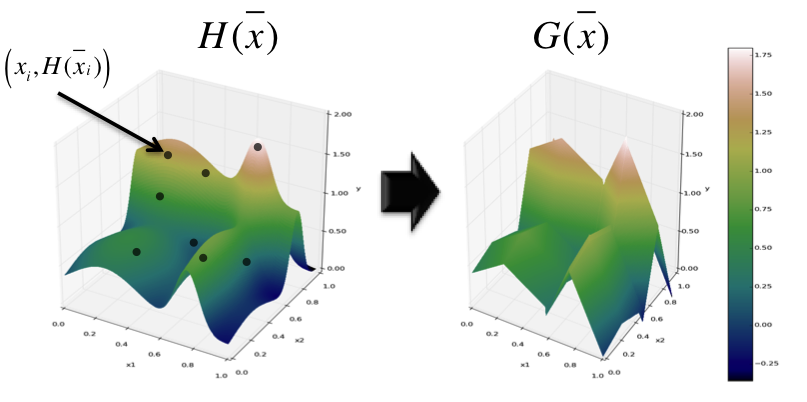
\includegraphics[width=1.0\textwidth]  {pics/ROMexampleOfPhysicalSystem.png}
  \caption{Example of reduced order model representation of physical system (regression).}
  \label{fig:ROMexampleOfPhysicalSystem}
\end{figure}

Two characteristics of these models
are generally assumed (even if exceptions are possible):
\begin{enumerate}
  \item The higher the number of realizations in the training sets, the
higher is the accuracy of the prediction performed by the ROM is. This
statement is true for most of the cases, although some ROMs might be
subject to the over-fitting issues. The over-fitting phenomenon is not
analyzed in this thesis, since its occurrence highly depends on the
algorithm type, and, hence, the problem needs to be analyzed for all
the large number of ROM types available;
  \item The smaller the size of the input (uncertain) domain with
  respect to the variability of the system response, the more likely the
  ROM is able to represent the system response space.
\end{enumerate}

\subsection{Reduced Order Modeling: Theory}
\label{sec:ROMsTheory}
To provide a very simple idea of a ROM, assume that the final
response space of a physical system is governed by the transfer
function $H \left (  \overline{x}\right)$ (see Section
~\ref{sub:mathBackground}), which, from a practical point of
view, represents the outcome of the system based on the initial
conditions  $\overline{x}$. Now, sample the domain of variability of the
initial conditions $\overline{x}$ to create a
set of $N$ realizations of the input and response space $ \left ( \left (
\overline{x}_{i}, H \left (  \overline{x}_{i}\right) \right), i=1,N \right)$,
named ``training'' set. Based on the data set generated, it is possible
to construct a mathematical representation $G\left ( \overline{x}:
\overline{x}_{i}\right)$ of the
real system $H \left (  \overline{x}\right)$, which will approximate its
response (see Figure~\ref{fig:ROMexampleOfPhysicalSystem}):
\begin{equation}
\label{eq:regressor}
G\left ( \overline{x} \right ):\overline{x}_{i} \rightarrow G\left ( \overline{x}_{i} \right ) \cong H\left ( \overline{x}_{i} \right )
\end{equation}
The ROMs reported above are generally named ``regressors'', among
which all the most common data fitting algorithms are found (e.g.,
least square for construction of linear models).

An important class of ROMs for the work presented here after is the
one containing the so called ``classifiers''. A classifier is a ROM that is
capable of representing the system behavior from a binary point of
view (e.g., event happened/not happened or failure/success). It is a
model (set of equations) that identifies to which category an object
belongs in the feature (input) space. Referring to the example that
brought to Equation ~\ref{eq:regressor}, a classifier can be formally represented as follows (see
Figure~\ref{fig:ROMClassifierExampleOfPhysicalSystem}):
\begin{figure}[h!]
  \centering
  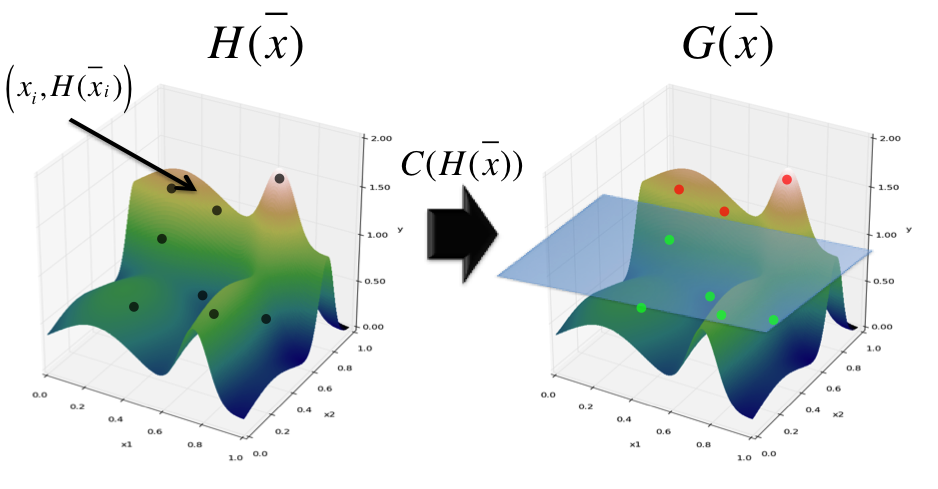
\includegraphics[width=1.0\textwidth]  {pics/ROMClassifierExampleOfPhysicalSystem.png}
  \caption{Example of reduced order model representation of physical system (classifier).}
  \label{fig:ROMClassifierExampleOfPhysicalSystem}
\end{figure}

\begin{equation}
\label{eq:classifier}
G\left ( \overline{x} \right ):\overline{x}_{i} \rightarrow G\left ( \overline{x}_{i} \right ) \cong
C \left ( H\left ( \overline{x}_{i} \right ) \right )
\end{equation}

The function $C\left (  H\left ( \overline{x}_{i}  \right ) = \overline{\theta}
\right ) $ is the so called ``goal'' function that is able to recast the
response of the system $H\left ( \overline{x}_{i}  \right )$ into a binary
form (e.g., failure/success). As an example, referring to
Figure~\ref{fig:ROMClassifierExampleOfPhysicalSystem}, the
``goal'' function would be:
\begin{equation}
\label{eq:goalFunctionClassifier}
C\left (   \overline{\theta}  \right ) = \left\{\begin{matrix}
1 & if \: \overline{\theta}>1.0 \\
0 &  if \: \overline{\theta} \leq 1.0
\end{matrix}\right.
\end{equation}
Hence, the ROM of type classifier $G\left (  \overline{x} \right )$  will operate in the space transformed through the ``goal''  function $C\left (   \overline{\theta}  \right )$.
\\The classifiers and regressors can be categorized into two main classes:
\begin{itemize}
  \item Model-based algorithms
  \item Data-based algorithms
\end{itemize}
In the first class, the created ROM aims to approximate the response
of the system as a function of the input parameters. These algorithms
construct a functional representation of the system. Examples of such ROM type are Support Vector Machines (SVMs), Kriging-based regressors, discriminant-based models, and polynomial chaos.

On the other side, data-based algorithms do not build a response-
function-based ROM but classify or predict the response of the
system from the neighborhood graph constructed from the training
data, without any dependencies on a particular prediction model.
These algorithms directly build a neighborhood structure as the
ROM (e.g., a relaxed Gabriel graph) on the initial training data. Examples of such ROM type are nearest neighbors and decision trees.

\textcolor{red}{\\It is important to NOTICE that RAVEN uses a Z-score normalization of the training data before 
  constructing most of the ROMs:
\begin{equation}
  \mathit{\mathbf{X}} = \frac{(\mathit{\mathbf{X}}-\mu )}{\sigma }
\end{equation} 
 } 
In order to understand which ROMs get trained with data normalized by the previous reported normalization approach, please refer to the RAVEN user manual \cite{RAVENuserManual}.

\subsubsection{Gaussian Process Models}
\label{sec:GPM}
Gaussian Processes (GPs)~\cite{Rasmussen_GPM} are algorithms that extend multivariate Gaussian distributions to infinite dimensionality. A Gaussian process generates a data set located throughout some domain such that any finite subset of the range follows a multivariate Gaussian distribution. Now, the n observations in an arbitrary data set, $y={y_1,\ldots,y_n}$, can always be imagined as a single point sampled from some multivariate ($n$-variate) Gaussian distribution.
What relates one observation to another in such cases is just the covariance function, $k(x,x')$. A popular choice is the squared exponential:
\begin{equation}
k(x,x')=\sigma_{f}^{2}  exp \left [ \frac{-(x-x')^2}{2 l^2} \right ]
\end{equation}
where the maximum allowable covariance is defined as $\sigma_{f}^{2}$; this should be high for functions that cover a broad range on the y axis. If $x \simeq x'$, then $k(x,x')$ approach this maximum meaning $f(x)$ is very correlated to $f(x')$. On the other hand, if $x$ is very distant from $x'$, then $k(x,x' ) \simeq 0$ (i.e., the two points cannot see each other.
So, for example, during interpolation at new $x$ values, distant observations will have negligible effect). How much effect this separation has will depend on the length parameter $l$.
Each observation $y$ can be thought of as related to an underlying function $f(x)$ through a Gaussian noise model:
\begin{equation}
y=f(x)+N(0,\sigma_{n}^{2})
\end{equation}
The new kernel function can be written as:
\begin{equation}
k(x,x')=\sigma_{f}^{2}  exp \left [ \frac{-(x-x')^2}{2 l^2} \right ] + \sigma_{n}^{2} \delta(x,x')
\end{equation}
So given $n$ observations $y$, the objective is to predict the value $y_*$ at the new point $x_*$. This process is performed by following this sequence of steps:
\begin{enumerate}
\item Calculate three matrices:
\begin{equation}
K=\begin{bmatrix}
k(x_1,x_1) &  \ldots & k(x_1,x_n)\\
\vdots  & \ddots &\vdots  \\
k(x_n,x_1) &  \ldots & k(x_n,x_n)
\end{bmatrix}
\end{equation}
\begin{equation}
K_*= \begin{bmatrix}
k(x_*,x_1) & \ldots & k(x_*,x_n)
\end{bmatrix}
\end{equation}
\begin{equation}
K_{**}=k(x_*,x_*)
\end{equation}
\item The basic assumption of GPM is that:
\begin{equation}
\begin{bmatrix}
y\\
y_*
\end{bmatrix}
=\mathcal{N}(0,\begin{bmatrix}
K & K_{*}^{T}\\
K_* & K_{**}
\end{bmatrix})
\end{equation}
\item The estimate $\bar{y_*} $ for $y_*$ is the mean of this distribution
\begin{equation}
\bar{y_*}=K_* K^{-1}y
\end{equation}
\item The uncertainty associated to the estimate $\bar{y_*} $ can be expressed in terms of variance of  $y_*$:
\begin{equation}
var(y_*)=K_{**}-k_* K^{-1} K_{*}^{T}
\end{equation}
\end{enumerate}

\subsubsection{Support Vector Machines}
\label{sec:SVM}
The Support Vector Machine (SVM)~\cite{SVM_Burges} classifier is a methodology that aims to determine the optimal separation hyperplane between data sets having different labels.
The training data consist of $N$ data points $(x_i,y_i)$ $i=1,\ldots,N$ where $x_i \in \mathbb{R}^M$ and $y_i \in {-1,1}$.
Assuming a linear property of the hyperplane  then its definition is:
\begin{equation}
\left \{ x: f(x)=x^T\beta+\beta_0=0 \right \}
\end{equation}
where $\beta$ is a unit vector.

The SVM parameters $\beta$ and $\beta_0$  are determined by solving this optimization problem:
\begin{equation}
\left\{\begin{matrix}
\underset{\beta,\beta_0}{min} \left \| \beta \right \|\\
\text{subject to } y_i(x_{i}^{T}\beta+\beta_0)\geq 1 , \quad i=1,\dots,N
\end{matrix}\right.
\end{equation}

Once the SVM parameters $\beta$ and $\beta_0$ are determined then the classification of a new point $\bar{x}$ is given by:
\begin{equation}
G(\bar{x})=sign(\bar{x}^T\beta+\beta_0)
\end{equation}


\subsubsection{KNN Classifier and KNR Regressor}
\label{sec:KNN_KNR}
The K Nearest Neighbor algorithm~\cite{altman_KNN} (KNN) is a non-parametric method used for both regression and classification. The only input parameter is the variable $K$ which indicates the number of neighbors to be considered in the classification/regression process. The special case where the class is predicted to be the class of the closest training sample (i.e. when $K = 1$) is called the nearest neighbor algorithm. In binary (two class) classification problems, it is helpful to choose k to be an odd number as this avoids tied votes. The output depends on whether KNN is used for classification or regression:
\begin{itemize}
\item In KNN classification, the output is a class membership. An object is classified by a majority vote of its neighbors, with the object being assigned to the class most common among its $K$ nearest neighbors ($K$ is a positive integer, typically small). If $K = 1$, then the object is simply assigned to the class of that single nearest neighbor.
\item In KNN regression, the output is the property value for the object. This value is the average of the values of its $K$ nearest neighbors.
\end{itemize}
Both for classification and regression, it can be useful to assign weight to the contributions of the neighbors, so that the nearer neighbors contribute more to the average than the more distant ones. For example, a common weighting scheme consists in giving each neighbor a weight of $1/d$, where $d$ is the distance to the neighbor.

\subsubsection{Multi-Dimensional Interpolation}
\label{sec:ND_interp}
This section covers the methods that have been implemented in the CROW statistical library:
\begin{itemize}
\item Shepard's Method (see Section~\ref{sec:shepard})
\item Multi-Dimensional Spline method (see Section~\ref{sec:ND_spline}).
\end{itemize}

These two methods are interpolation methods that can be used in any dimension.
In RAVEN they are employed in two major applications:
\begin{enumerate}
\item ROMs
\item Multi-dimensional distributions.
\end{enumerate}
For both applications, given a set of $N$ data points $ (x_i,u_i )$  $i=1,\ldots,N$ where $x_i$ are the coordinate in the input space $D \subset \mathbb{R}^M$ and $u_i \in \mathbb{R}$ is the outcome, the methods predicts the outcome $\tilde{u}$ for a new coordinate $\tilde{x}\in \mathbb{R}^n$.


\paragraph{Shepard's Method}
\label{sec:shepard}
The Shepard interpolator~\cite{Shepard} is also know as Inverse Distance Weighting (IDW) interpolator.
The starting point is a set of $N$ data points $ (x_i,u_i )$ for $i=1,\ldots,N$.
The Inverse-Weight interpolator can be represented as a function $f_{IDW}(x)$ that, given a new coordinate in the input space $x$, generates a prediction on $u$ such that
\begin{equation}
u:x \in \mathbb{R}^M \rightarrow f_{IDW}(x) \in \mathbb{R}
\end{equation}
based on the distance $d(x,x_i)$ in the euclidean space between $x$ and $x_i$.

Such prediction $u=f_{IDW}(x)$ is performed by summing all data points $x_i$ $i=1,\ldots,N$ weighted by a weighting parameter $w_i (x)$ as follows:
\begin{equation}
f_{IDW}(x) =
\left\{
\begin{matrix}
\sum_{i=1}^{N} w(x_i) u_i &  \text{if } d(x,x_i) \neq 0 \\
 u_i &  \text{if } d(x,x_i) = 0
\end{matrix}\right.
\end{equation}
where
\begin{equation}
w(x_i) =\frac{w_i}{\sum_{i=1}^{N} w_i}
\end{equation}
and
\begin{equation}
w_i = \left ( \frac{1}{d(x,x_i)} \right )^p
\end{equation}
Large values of $p$ assign greater weight $w_i$ to data points $x_i$ closest to $x$, with the result turning into a mosaic of tiles (i.e., Voronoi diagram) with nearly constant interpolated value.

\paragraph{Multi-Dimensional Spline}
\label{sec:ND_spline}
The Multi-Dimensional Spline (MDS)~\cite{MD_spline} is a method that requires the sampled points $x_i$ to be lying in multi-dimensional cartesian grid.
A generic grid $\Delta_m$ for each dimension $m$ will be indicated as follows:
\begin{equation}
\Delta_m = \{x_{0_m},x_{1_m},\ldots,x_{p_m}\} \text{ for } m=1,\ldots,M
\end{equation}
This methods construct a $M$-dimensional cubic spline so that, given a coordinate in the input space $x=(x_1,x_2,\ldots,x_M)$, generates a prediction on $u$ such that
\begin{equation}
u:x \in \mathbb{R}^M \rightarrow f_{MDS}(x) \in \mathbb{R}
\end{equation}
where
\begin{equation}
f_{MDS}(x)=\sum_{i_1=1}^{p_1+3} \sum_{i_2=1}^{p_2+3} \ldots \sum_{i_M=1}^{p_M+3} c_{i_1,i_2,\ldots,i_p} \prod_{m=1}^{M} u_{i_j} (x_m)
\end{equation}
where
\begin{equation}
u_{i_j} (x_m) = \Phi\left ( \frac{x_m-x_{0_m}}{h_j}+2-i_j  \right )
\end{equation}

The cubic kernel $\Phi(t)$ is defined as:
\begin{equation}
\Phi(t) = \left\{\begin{matrix}
(2-\left | t \right |)^3 & 1\leq \left | t \right |\leq 2 \\
4-6\left | t \right |^2+3\left | t \right |^3 & \left | t \right |\leq 1\\
0 & \text{elsewhere}
\end{matrix}\right.
\end{equation}

The set of $\prod_{m=1}^{M}(p_m+3)$ coefficients $c_{i_1,i_2,\ldots,i_p}$  is determined when the interpolator is initialized.

%%%%%%%%%%%%%%%%
\subsection{Reduced Order Modeling through RAVEN}
\label{subsub:ROMraven}
The goals of this section are about learning how to:
 \begin{enumerate}
   \item Set up a sampling strategy to construct multiple ROMs, perturbing a driven code
   \item Train the different ROMs with the data-set obtained by the applied sampling strategy;
   \item Use the same sampling strategy, perturbing the ROMs
   \item Plot the responses of the driven code and ROMs, respectively.
\end{enumerate}
In order to accomplish these tasks, the following RAVEN \textbf{Entities} (XML blocks in the input files) need to be defined:
\begin{enumerate}
   \item \textbf{\textit{RunInfo}}:
\begin{lstlisting}[style=XML,morekeywords={arg,extension,pauseAtEnd,overwrite}]
  <RunInfo>
    <JobName>Chapter-IX/ROMConstruction</JobName>
    <Sequence>
        sample,trainROMGaussianProcess,trainROMsvm,
        trainROMinverse,sampleROMGaussianProcess,
        sampleROMInverse,sampleROMsvm,writeHistories
    </Sequence>
    <WorkingDir>ROMConstruction</WorkingDir>
    <batchSize>12</batchSize>
  </RunInfo>
\end{lstlisting}
   As in the other examples, the the \textit{RunInfo} \textbf{Entity} is intended  to set up the analysis sequence that
   needs to be performed. In this specific case, eight steps  (\xmlNode{Sequence}) are going to be sequentially run
   using eight processors (\xmlNode{batchSize}).
   \\In the first step, the original physical model is going to be sampled. The obtained results are going to be used to
   train three different ROMs.These ROMs are sampled by the same strategy used in the first step in order to compare the
   ROMs' responses with the ones coming from the original physical model.
   \item \textbf{\textit{Files}}:
\begin{lstlisting}[style=XML,morekeywords={arg,extension,pauseAtEnd,overwrite}]
  <Files>
    <Input name="referenceInput.xml" type="input">referenceInput.xml</Input>
  </Files>
\end{lstlisting}
   Since the driven code uses a single input file, the original input is placed in this section. As detailed in the user manual
   the attribute  \xmlAttr{name} represents the alias that is going to be
   used in all the other input blocks in order to refer to this file.
   \item \textbf{\textit{Models}}:
\begin{lstlisting}[style=XML,morekeywords={arg,extension,pauseAtEnd,overwrite}]
  <Models>
    <Code name="testModel" subType="GenericCode">
      <executable>
       ../physicalCode/analyticalbateman/AnalyticalDplMain.py
      </executable>
      <clargs arg="python" type="prepend"/>
      <clargs arg="" extension=".xml" type="input"/>
      <clargs arg="" extension=".csv" type="output"/>
      <prepend>python</prepend>
    </Code>
    <ROM name="ROMGaussianProcess" subType="SciKitLearn">
      <Features>sigma-A,sigma-B,decay-A,decay-B</Features>
      <Target>A,B</Target>
      <SKLtype>GaussianProcess|GaussianProcess</SKLtype>
      <regr>quadratic</regr>
      <theta0>10</theta0>
    </ROM>
    <ROM name="ROMsvm" subType="SciKitLearn">
      <Features>sigma-A,sigma-B,decay-A,decay-B</Features>
      <Target>A,B</Target>
      <SKLtype>svm|SVR</SKLtype>
      <kernel>rbf</kernel>
      <C>50.0</C>
      <tol>0.000001</tol>
    </ROM>
    <ROM name="ROMinverse" subType="NDinvDistWeight">
      <Features>sigma-A,sigma-B,decay-A,decay-B</Features>
      <Target>A,B</Target>
      <p>3</p>
    </ROM>
  </Models>
\end{lstlisting}
 As mentioned above, the goal of this example is the employment of
 a sampling strategy in order to construct multiple types of ROMs.
 \\Indeed, in addition to the previously explained Code
 model,
 three different ROMs (GP, SVM and IDW) are here specified. The ROMs will be
 constructed (``trained'') through the data-set generated by the sampling of the physical model. Once trained, they are going
 to be used in place of the original physical model.
 \\As it can be seen,
 the ROMs will be constructed considering four features ($sigma-A,\,sigma-B,\, decay-A \,,and \, decay-B$) and two targets
 ($A \, and \, B$).
   \item \textbf{\textit{Distributions}}:
\begin{lstlisting}[style=XML]
  <Distributions>
      <Uniform name="sigma">
          <lowerBound>0</lowerBound>
          <upperBound>1000</upperBound>
      </Uniform>
      <Uniform name="decayConstant">
          <lowerBound>0.00000001</lowerBound>
          <upperBound>0.0000001</upperBound>
      </Uniform>
  </Distributions>
\end{lstlisting}
  In the Distributions XML section, the stochastic model for the
  uncertainties are reported. In
  this case two distributions are defined:
  \begin{itemize}
    \item $sigma \sim \mathbb{U}(0,1000)$, used to model the uncertainties
    associated with  the Model \textit{sigma-A} and \textit{sigma-B};
    \item  $decayConstant \sim \mathbb{U}(1e-8,1e-7)$,  used to
    model the uncertainties
    associated with  the Model \textit{decay-A} and \textit{decay-B}.
  \end{itemize}
   \item \textbf{\textit{Samplers}}:
\begin{lstlisting}[style=XML,morekeywords={arg,extension,pauseAtEnd,overwrite}]
  <Samplers>
    <Grid name="grid">
      <variable name="sigma-A">
        <distribution>sigma</distribution>
        <grid construction="equal" steps="5" type="CDF">0.01 0.99</grid>
      </variable>
      <variable name="decay-A">
        <distribution>decayConstant</distribution>
        <grid construction="equal" steps="5" type="CDF">0.01 0.99</grid>
      </variable>
      <variable name="sigma-B">
          <distribution>sigma</distribution>
          <grid construction="equal" steps="5" type="CDF">0.01 0.99</grid>
      </variable>
      <variable name="decay-B">
          <distribution>decayConstant</distribution>
          <grid construction="equal" steps="5" type="CDF">0.01 0.99</grid>
      </variable>
    </Grid>
  </Samplers>
\end{lstlisting}
  To obtain the data-set through which the ROMs are going to be
  constructed, a \textit{Grid} sampling approach is here employed.
   \item \textbf{\textit{DataObjects}}:
\begin{lstlisting}[style=XML,morekeywords={arg,extension,pauseAtEnd,overwrite}]
  <DataObjects>
    <PointSet name="samples">
      <Input>sigma-A,sigma-B,decay-A,decay-B</Input>
      <Output>A,B,C,D</Output>
    </PointSet>
    <HistorySet name="histories">
        <Input>sigma-A,sigma-B,decay-A,decay-B</Input>
        <Output>A,B,C,D,time</Output>
    </HistorySet>
    <PointSet name="inputPlaceHolder">
      <Input>sigma-A,sigma-B,decay-A,decay-B</Input>
      <Output>OutputPlaceHolder</Output>
    </PointSet>
    <PointSet name="samplesGP">
      <Input>sigma-A,sigma-B,decay-A,decay-B</Input>
      <Output>A,B</Output>
    </PointSet>
    <PointSet name="samplesInverse">
      <Input>sigma-A,sigma-B,decay-A,decay-B</Input>
      <Output>A,B</Output>
    </PointSet>
    <PointSet name="samplesSVM">
      <Input>sigma-A,sigma-B,decay-A,decay-B</Input>
      <Output>A,B</Output>
    </PointSet>
  </DataObjects>
\end{lstlisting}
  Int this block, six \textit{DataObjects} are defined: 1) PointSet
  named ``samples'' used to collect the final outcomes of the code, 2)
  HistorySet named ``histories'' in which the full time responses of the
  variables $A,B,C,D$ are going to be stored, 3) PointSet named
  ``inputPlaceHolder'' used in the \textit{role} of \xmlNode{Input} for the ROMs sampling;
  4) PointSet named ``samplesGP'' used to collect the final outcomes (sampling) of the GP ROM;
  5) PointSet named ``samplesInverse'' used to collect the final outcomes (sampling) of the IDW ROM;
  6) PointSet named ``samplesSVM'' used to collect the final outcomes (sampling) of the SVM ROM.
 %%%%%%%%%%%%%%%%%%%%%%%%%%%%%%%%%%%%%%%%%%%%%%%%%%%%%%%%%%
 %%%%%%%%%%%%%%%%%%%%%%%%%%%%%%%%%%%%%%%%%%%%%%%%%%%%%%%%%%
 %figure samples
 \begin{figure}[h!]
  \centering
  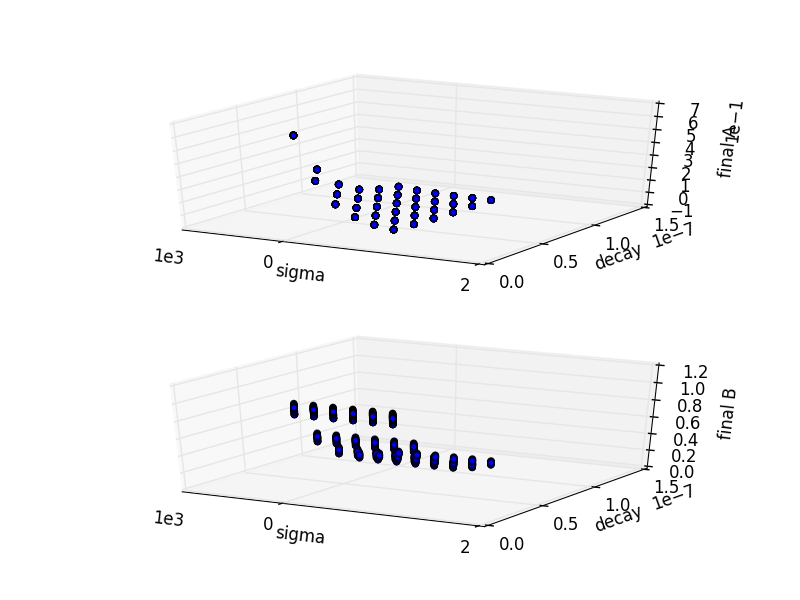
\includegraphics[scale=0.7]{pics/samplesplot3d.png}
  \caption{Plot of the samples generated by the Grid sampling for variables $A,B$.}
  \label{fig:ROMgrid_pointsets}
 \end{figure}
 %%%%%%%%%%%%%%%%%%%%%%%%%%%%%%%%%%%%%%%%%%%%%%%%%%%%%%%%%%
 %%%%%%%%%%%%%%%%%%%%%%%%%%%%%%%%%%%%%%%%%%%%%%%%%%%%%%%%%%
   \item \textbf{\textit{Steps}}:
\begin{lstlisting}[style=XML,morekeywords={arg,extension,pauseAtEnd,overwrite}]
  <Steps>
    <MultiRun name="sample">
      <Input class="Files" type="input">referenceInput.xml</Input>
      <Model class="Models" type="Code">testModel</Model>
      <Sampler class="Samplers" type="Grid">grid</Sampler>
      <Output class="DataObjects" type="PointSet">samples</Output>
      <Output class="DataObjects" type="HistorySet">histories</Output>
    </MultiRun>
    <MultiRun name="sampleROMGaussianProcess">
      <Input class="DataObjects" type="PointSet">inputPlaceHolder</Input>
      <Model class="Models" type="ROM">ROMGaussianProcess</Model>
      <Sampler class="Samplers" type="Grid">grid</Sampler>
      <Output class="DataObjects" type="PointSet">samplesGP</Output>
    </MultiRun>
    <MultiRun name="sampleROMInverse">
      <Input class="DataObjects" type="PointSet">inputPlaceHolder</Input>
      <Model class="Models" type="ROM">ROMinverse</Model>
      <Sampler class="Samplers" type="Grid">grid</Sampler>
      <Output class="DataObjects" type="PointSet">samplesInverse</Output>
    </MultiRun>
    <MultiRun name="sampleROMsvm">
      <Input class="DataObjects" type="PointSet">inputPlaceHolder</Input>
      <Model class="Models" type="ROM">ROMsvm</Model>
      <Sampler class="Samplers" type="Grid">grid</Sampler>
      <Output class="DataObjects" type="PointSet">samplesSVM</Output>
    </MultiRun>
    <RomTrainer name="trainROMGaussianProcess">
      <Input class="DataObjects" type="PointSet">samples</Input>
      <Output class="Models" type="ROM">ROMGaussianProcess</Output>
    </RomTrainer>
    <RomTrainer name="trainROMsvm">
      <Input class="DataObjects" type="PointSet">samples</Input>
      <Output class="Models" type="ROM">ROMsvm</Output>
    </RomTrainer>
    <RomTrainer name="trainROMinverse">
      <Input class="DataObjects" type="PointSet">samples</Input>
      <Output class="Models" type="ROM">ROMinverse</Output>
    </RomTrainer>
    <IOStep name="writeHistories" pauseAtEnd="True">
        <Input   class="DataObjects"      type="HistorySet">histories</Input>
        <Input   class="DataObjects"      type="PointSet">samples</Input>
        <Input   class="DataObjects"      type="PointSet">samplesGP</Input>
        <Input   class="DataObjects"      type="PointSet">samplesInverse</Input>
        <Input   class="DataObjects"      type="PointSet">samplesSVM</Input>
        <Output class="OutStreams" type="Plot">samplesPlot3D</Output>
        <Output class="OutStreams" type="Plot">samplesPlot3DROMgp</Output>
        <Output class="OutStreams" type="Plot">samplesPlot3DROMsvm</Output>
        <Output class="OutStreams" type="Plot">samplesPlot3DROMinverse</Output>
        <Output class="OutStreams" type="Plot">historyPlot</Output>
        <Output class="OutStreams" type="Print">samples</Output>
        <Output class="OutStreams" type="Print">histories</Output>
    </IOStep>
  </Steps>
\end{lstlisting}
  %%%%%%%%%%%%%%%%%%%%%%%%%%%%%%%%%%%%%%%%%%%%%%%%%%%%%%%%%%
 %figure samples
 \begin{figure}[h!]
  \centering
  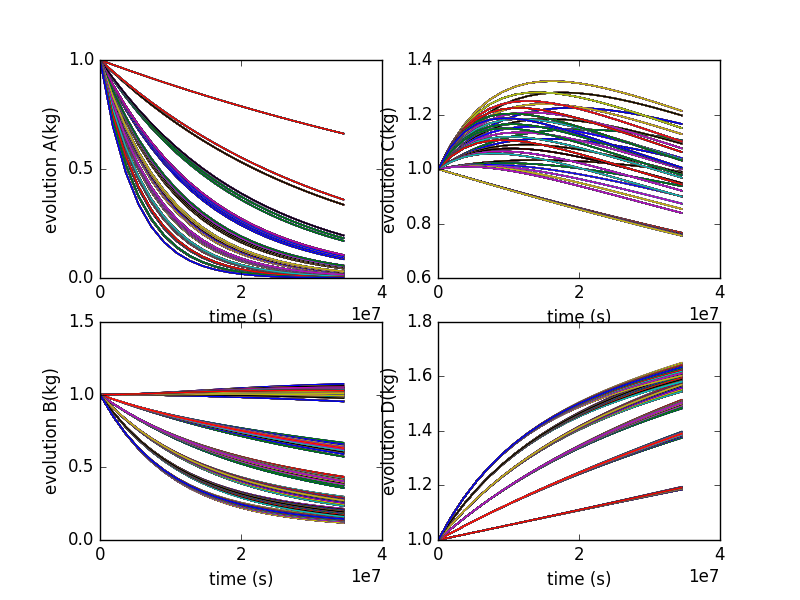
\includegraphics[scale=0.7]{pics/reducedOrderModelingHistoriesPhysicalModel.png}
  \caption{Plot of the histories generated by the Grid method for variables $A,B,C,D$.}
  \label{fig:ROMgrid_histories}
 \end{figure}
   %%%%%%%%%%%%%%%%%%%%%%%%%%%%%%%%%%%%%%%%%%%%%%%%%%%%%%%%%%
 %figure samples
 \begin{figure}[h!]
  \centering
  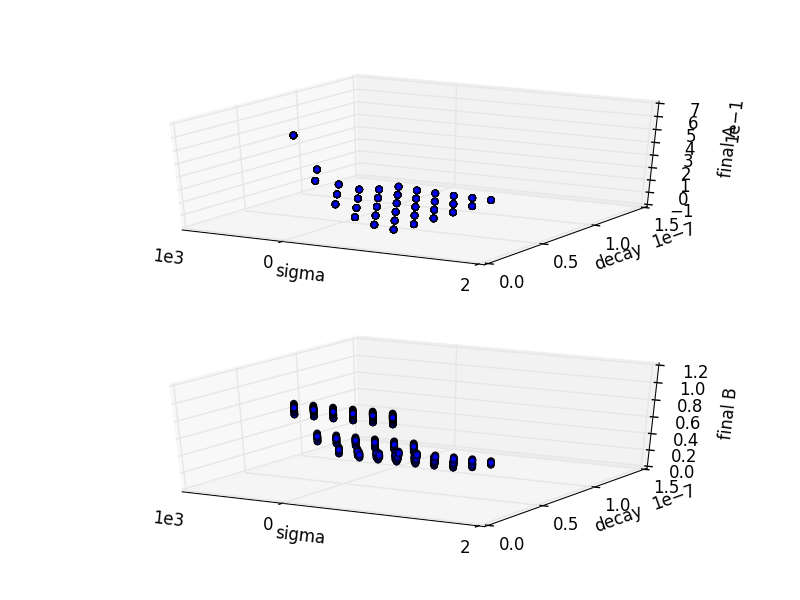
\includegraphics[scale=0.7]{pics/samplesPlot3DROMgp_scatter-scatter.png}
  \caption{Plot of the samples generated by the Grid sampling applied on the Gaussian Process ROM for variables $A,B$}
  \label{fig:ROMgp_samples}
 \end{figure}
 %%%%%%%%%%%%%%%%%%%%%%%%%%%%%%%%%%%%%%%%%%%%%%%%%%%%%%%%%%
 %%%%%%%%%%%%%%%%%%%%%%%%%%%%%%%%%%%%%%%%%%%%%%%%%%%%%%%%%%
   Finally, all the previously defined \textbf{Entities} can be combined in
   the \xmlNode{Steps} block. As inferable,
   eight \xmlNode{Steps} have been inputted:
   \begin{itemize}
     \item \xmlNode{MultiRun} named ``sample'', used to run the multiple
     instances of the driven code and
     collect the outputs in the two \textit{DataObjects}. As it can be
     seen, the \xmlNode{Sampler} is inputted to communicate to the
     \textit{Step} that the driven code needs to
     be perturbed through the Grid sampling strategy;
     \item \xmlNode{RomTrainer} named ``trainROMGaussianProcess'', used to construct (``train'')
     the GP ROM, based on the data-set generated in the  ``sample'' \textbf{Step};
     \item \xmlNode{RomTrainer} named ``trainROMsvm'', used to construct (``train'')
     the SVM ROM, based on the data-set generated in the  ``sample'' \textbf{Step};
     \item \xmlNode{RomTrainer} named ``trainROMinverse'', used to construct (``train'')
     the IDW ROM, based on the data-set generated in the  ``sample'' \textbf{Step};
     \item \xmlNode{MultiRun} named ``sampleROMGaussianProcess'', used to run the multiple
     instances of the previously constructed GP ROM and
     collect the outputs in the PointSet \textit{DataObject}. As it can be
     seen, the same \xmlNode{Sampler} used for perturbing the original model is here used.
     \item \xmlNode{MultiRun} named ``sampleROMsvm'', used to run the multiple
     instances of the previously constructed Support Vector Machine ROM and
     collect the outputs in the PointSet \textit{DataObject}. As it can be
     seen, the same \xmlNode{Sampler} used for perturbing the original model is here used.
     \item \xmlNode{MultiRun} named ``sampleROMInverse'', used to run the multiple
     instances of the previously constructed Inverse Distance Weight ROM and
     collect the outputs in the PointSet \textit{DataObject}. As it can be
     seen, the same \xmlNode{Sampler} used for perturbing the original model is here used.
     \item  \xmlNode{IOStep} named ``writeHistories'', used to 1) export
     the ``histories'' and ``samples''  \textit{DataObjects}
     \textbf{Entity} in a CSV file and 2) plot the responses of the sampling performed on the physical model, GP ROM,
     SVM ROM and IDW ROM in  PNG files and on the screen.
   \end{itemize}
\end{enumerate}

  %figure samples
 \begin{figure}[h!]
  \centering
  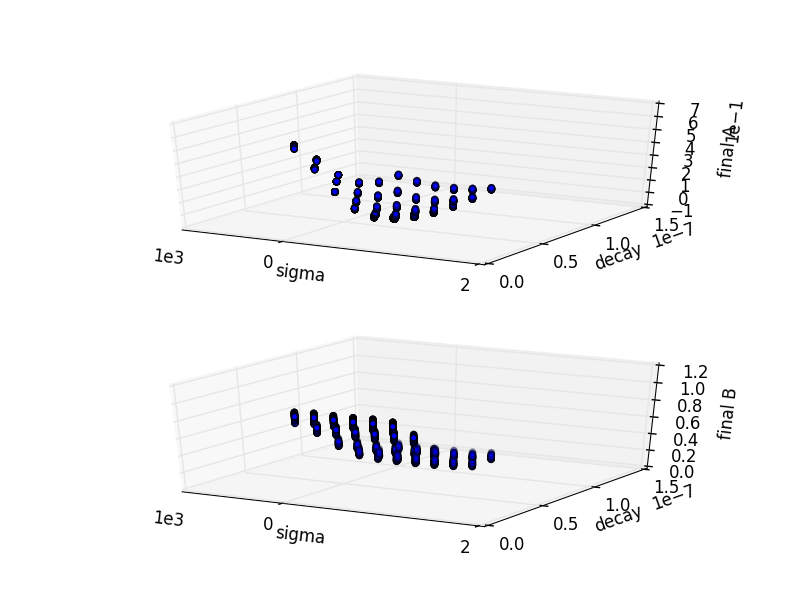
\includegraphics[scale=0.7]{pics/samplesPlot3DROMsvm_scatter-scatter.png}
  \caption{Plot of the samples generated by the Grid sampling applied on the Support Vector Machine ROM for variables $A,B$}
  \label{fig:ROMsvm_samples}
 \end{figure}
 %%%%%%%%%%%%%%%%%%%%%%%%%%%%%%%%%%%%%%%%%%%%%%%%%%%%%%%%%%
  %%%%%%%%%%%%%%%%%%%%%%%%%%%%%%%%%%%%%%%%%%%%%%%%%%%%%%%%%%
  %figure samples
 \begin{figure}[h!]
  \centering
  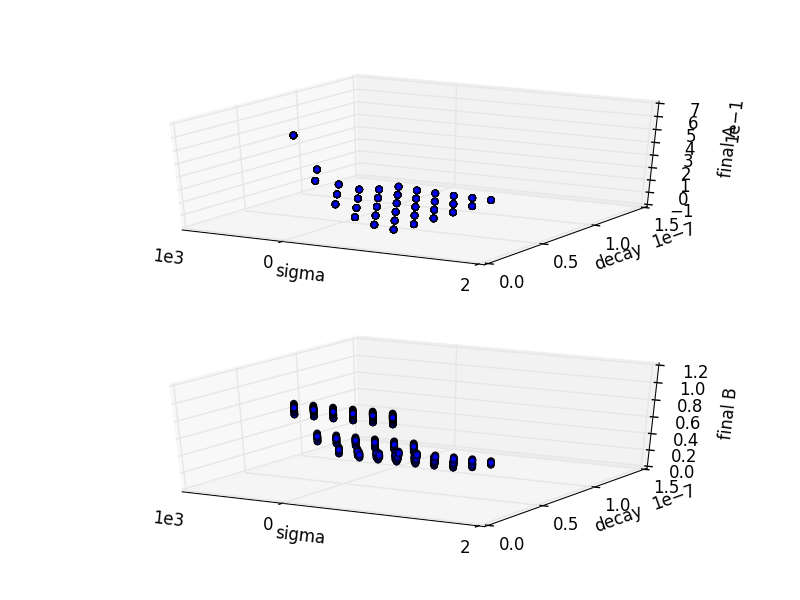
\includegraphics[scale=0.7]{pics/samplesPlot3DROMinverse_scatter-scatter.png}
  \caption{Plot of the samples generated by the Grid sampling applied on the Inverse Distance Weight ROM for variables $A,B$}
  \label{fig:ROMinverse_samples}
 \end{figure}
 %%%%%%%%%%%%%%%%%%%%%%%%%%%%%%%%%%%%%%%%%%%%%%%%%%%%%%%%%%
 Figure \ref{fig:ROMgrid_histories}
 shows the evolution of the outputs $A,B,C,D$ under uncertainties.
 Figure \ref{fig:ROMgrid_pointsets} shows the final responses  of $A and B$
 of the sampling employed using the driven code.

Figures \ref{fig:ROMgp_samples}, \ref{fig:ROMsvm_samples} and \ref{fig:ROMinverse_samples}  show the final responses  of $A and B$ of the sampling employed using the Gaussian Process, Support Vector Machines and Inverse Distance Weight ROMs, respectively.
It can be clearly noticed that the responses of the ROMs perfectly match the outcomes coming from the original model (see Figure   \ref{fig:ROMgrid_pointsets}).









\section{RAVEN Theory by way of Examples: Statistical analysis}
In order to perform a complete analysis of a system under uncertanties,
it is crucial to be able to compute all the statistical moments of multiple
Figures of Merit (FOMs). In addition, it is essential to identify the correlation
among different FOMs toward a specific input space. 
\\RAVEN is able to compute all the most important statistical FOMs, which
represent the base of each sensitivity and uncertainty quantification analysis,
such as:
\begin{enumerate}
  \item \textit{Expected Value};
  \item \textit{Standard Deviation};
  \item \textit{Variance};
  \item \textit{variationCoefficient}; 
  \item \textit{Skewness};
  \item \textit{Kurtosis};  
  \item \textit{Median}; 
  \item \textit{Percentile}.
\end{enumerate} 
In addition, RAVEN fully supports the computation of all the FOMs that are aimed to
``measure'' the correlation among variables/parameters:
\begin{enumerate}
  \item \textit{Covariance matrix};
  \item \textit{Normalized Sensitivity  matrix};
  \item \textit{Variance Dependent Sensitivity  matrix};
  \item \textit{Sensitivity matrix}; 
  \item \textit{Pearson matrix}.
\end{enumerate} 
In this section all of these features are going to be analyzed, explaining the theory behind it
by way of applied RAVEN examples.
\subsection{Statistical analysis theory}
One of the most assessed way to investigate the impact of the intrinsic variation of the input space, is through the computation of 
statistical moments and linear correlation figure of merits. 
\\As stated in the previous chapters, RAVEN employs several different sampling methodologies in order to explore
the response of a physical (and not) model under uncertainties. Hence, in order to correctly compute the statistical FOMs, subject
of this section, a weighting approach needs to be used. Each \textit{Sampler} in RAVEN is able to attribute to each ``sample'' (i.e.
realization in the input/uncertain space) a \textbf{weight} that is aimed to represent the \textit{importance} of the particular
combination of input values from a statistical point of view (e.g. reliability weights). These weights are then used in sub-sequential
steps in order to compute the previously listed statistical moments and correlation metrics.
\\In the following sub-sections, the formulation of these statistical moments is reported.
\subsubsection{Expected Value}
The expected value concept represents one of the most fundamental metrics in probability theory. The expected value of a 
real-valued random variable represents a measurement of the center of the distribution (mean) of the random variable. 
From a practical point of view, the expected value of a discrete random variable is the probability-weighted average of all possible values of the subjected variable. Formally, the expected value of a random variable $X$
\begin{equation}
\begin{matrix}
\mathbb{E}(X) = \mu = \sum_{x \in \chi} x \times pdf_{X}(x) & if X \, discrete \\ 
\\ 
\mathbb{E}(X) = \mu = \int_{x \in \chi} x \times pdf_{X}(x) & \, if X \, \, continuous
\end{matrix}
\end{equation}
In RAVEN, the expected value (i.e. first central moment) is computed as follows:
\begin{equation}
\begin{matrix}
\mathbb{E}(X) = \mu \approx \overline{x} = \frac{1}{n} \sum_{i=1}^{n}  x_{i} & if \: random \: sampling \\ 
\\ 
\mathbb{E}(X) = \mu \approx \overline{x} = \frac{1}{V_{1}} \sum_{i=1}^{n} w_{i} \times x_{i}  & \, otherwise
\end{matrix}
\end{equation}
where 
\begin{itemize}
  \item $w_{i}$ is the weight associated with the sample $i$;
  \item $n$ are the total number of samples;
  \item $V_{1} = \sum_{i=1}^{n} w_{i}$.
\end{itemize}
\subsubsection{Standard Deviation and Variance}
The variance ($\sigma^{2}$) and standard deviation ($\sigma$) of $X$ are both measures of the spread of the distribution of the random variable about the 
mean. Simplistically, the variance measures how far a set of realizations of a random variable are spread out.
An equivalent measure is the square root of the variance, called the standard deviation. The standard deviation has the same dimension as the data, and hence is comparable to deviations from the mean.
\\Formally:
\begin{equation}
  \begin{matrix}
  \sigma^{2}(X)= \mathbb{E}\left(\left[X - \mathbb{E}(X)\right]^{2}\right) = \int_{x \in \chi} (x - \mu)^2 pdf(x) dx  & \, if X \, \, continuous \\
  \sigma^{2}(X)= \mathbb{E}\left(\left[X - \mathbb{E}(X)\right]^{2}\right)  = \sum_{x \in \chi} (x - \mu)^2 pdf(x)  & if X \, discrete
  \\
  \\ 
  \sigma(X)= \mathbb{E}\left(\left[X - \mathbb{E}(X)\right]\right)  = \sqrt{\sigma^{2}(X)}
  \end{matrix}
\end{equation}
In RAVEN, the variance (i.e. second central moment) and standard deviation are computed as follows:
\begin{equation}
\begin{matrix}
\mathbb{E}\left(\left[X - \mathbb{E}(X)\right]^{2}\right)  \approx  m_{2} = \frac{1}{n} \sum_{i=1}^{n}  (x_{i} - \overline{x})^{2} & if \: random \: sampling \\ 
\\ 
\\
\mathbb{E}\left(\left[X - \mathbb{E}(X)\right]^{2}\right)  \approx m_{2}  = \frac{1}{V_{1}} \sum_{i=1}^{n} w_{i} \times (x_{i} - \overline{x})^{2}  & \, otherwise
\\
\\
\mathbb{E}\left(\left[X - \mathbb{E}(X)\right]^{2}\right)  \approx s  =  \sqrt{m_{2}}
\end{matrix}
\end{equation}
where:
\begin{itemize}
  \item $w_{i}$ is the weight associated with the sample $i$;
  \item $n$ are the total number of samples;
  \item $V_{1} = \sum_{i=1}^{n} w_{i}$.
\end{itemize}
RAVEN performs an additional correction of variance to obtain an unbiased estimation  with respect to the sample-size~\cite{RimoldiniUnbiased}:
\begin{equation}
\begin{matrix}
\mathbb{E}\left(\left[X - \mathbb{E}(X)\right]^{2}\right)  \approx M_{2} = \displaystyle \frac{n}{n-1}m_{2} & & if \: random \: sampling
\\
\mathbb{E}\left(\left[X - \mathbb{E}(X)\right]^{2}\right)  \approx M_{2} = \frac{V_{1}^{2}}{V_{1}^{2} - V_{2}}m_{2} & \: otherwise
\end{matrix}
\end{equation}
\begin{equation}
S = \sqrt{M_{2}} 
\end{equation}
where:
\begin{itemize}
  \item $w_{i}$ is the weight associated with the sample $i$;
  \item $n$ are the total number of samples;
  \item $V_{1} = \sum_{i=1}^{n} w_{i}^{2}$;
\end{itemize}
It is important to notice that $S$ is not an unbiased estimator.

\subsubsection{Skewness}
The Skewness is a measure of the asymmetry of the distribution of a 
real-valued random variable about its mean. Negative skewness 
indicates that the tail on the left side of the distribution is longer or fatter 
than the right side.  Positive skewness indicates that the tail on the right 
side is longer or fatter than the left side. From a practical point of view, the 
skewness is useful to identify distortion  of the random variable with respect to
the Normal distribution function.
\\Formally, 
\begin{equation}
\gamma_{1} = \mathbb{E} \left [ \left ( \frac{X-\mu}{\sigma} \right )^{3} \right ] = \frac{ \mathbb{E}\left [ \left ( X-\mu \right )^{3} \right ]}{\left ( \mathbb{E}\left [ \left ( X-\mu \right )^{2} \right ] \right )^{3/2}}
\end{equation}
In RAVEN, the skewness is computed as follows:
\begin{equation}
\begin{matrix}
\mathbb{E} \left [ \left ( \frac{X-\mu}{\sigma} \right )^{3} \right ]  \approx \frac{m_{3}}{m_{2}^{3/2}} = \frac{  \frac{1}{n} \sum_{i=1}^{n}  (x_{i} - \overline{x})^{3} }{\left ( \frac{1}{n} \sum_{i=1}^{n}  (x_{i} - \overline{x})^{2} \right )^{3/2}} & if \: random \: sampling  
\\
\\
\mathbb{E} \left [ \left ( \frac{X-\mu}{\sigma} \right )^{3} \right ]  \approx \frac{m_{3}}{m_{2}^{3/2}} = \frac{  \frac{1}{V_{1}} \sum_{i=1}^{n} w_{i} \times (x_{i} - \overline{x})^{3} }{\left ( \frac{1}{V_{1}} \sum_{i=1}^{n}  w_{i} \times (x_{i} - \overline{x})^{2} \right )^{3/2}} &  \, otherwise
\end{matrix}
\end{equation}
where:
\begin{itemize}
  \item $w_{i}$ is the weight associated with the sample $i$;
  \item $n$ are the total number of samples;
  \item $V_{1} = \sum_{i=1}^{n} w_{i}$.
\end{itemize}
RAVEN performs an additional correction of skewness to obtain an unbiased estimation  with respect to the sample-size~\cite{RimoldiniUnbiased}:
\begin{equation}
\begin{matrix}
\mathbb{E} \left [ \left ( \frac{X-\mu}{\sigma} \right )^{3} \right ]  \approx \frac{M_{3}}{M_{2}^{3/2}}  = \displaystyle \frac{n^{2}}{(n-1)(n-2)}m_{3}\times \frac{1}{\left ( \displaystyle \frac{n}{n-1}m_{2}  \right )^{3/2}} & if \: random \: sampling  
\\
\\
\mathbb{E} \left [ \left ( \frac{X-\mu}{\sigma} \right )^{3} \right ]  \approx \frac{M_{3}}{M_{2}^{3/2}}  = \displaystyle \frac{V_{1}^{3}}{V_{1}^{3}-3V_{1}V_{2}+2V_{3}}m_{3} \times \frac{1}{\left ( \displaystyle \frac{V_{1}^{2}}{V_{1}^{2}-V_{2}}m_{2}  \right )^{3/2}} &  \, otherwise
\end{matrix}
\end{equation}
where:
\begin{itemize}
  \item $w_{i}$ is the weight associated with the sample $i$;
  \item $n$ are the total number of samples;
  \item $V_{1} = \sum_{i=1}^{n} w_{i}^{2}$;
  \item $V_{2} = \sum_{i=1}^{n} w_{i}^{2}$;
  \item $V_{3} = \sum_{i=1}^{n} w_{i}^{3}$.
\end{itemize}

\subsubsection{Excess Kurtosis}
The  Kurtosis~\cite{Abramowitz}  is the degree of peakedness of a distribution of a real-valued random variable. In a similar way to the concept of skewness, kurtosis describes the shape of the distribution. The Kurtosis is defined in order to
obtain a value of $0$ for a Normal distribution. If it is greater than zero, it indicates that the distribution is high peak; If it is smaller 
that zero, it testifies that the distribution is flat-topped.
\\Formally, the Kurtosis can be expressed as follows:
\begin{equation}
\gamma_{2} = \frac{ \mathbb{E}\left [ \left ( X-\mu \right )^{4} \right ]}{\left ( \mathbb{E}\left [ \left ( X-\mu \right )^{2} \right ] \right )^{2}} 
\end{equation}
In RAVEN, the kurtosis (excess) is computed as follows:
\begin{equation}
\begin{matrix}
\frac{ \mathbb{E}\left [ \left ( X-\mu \right )^{4} \right ]}{\left ( \mathbb{E}\left [ \left ( X-\mu \right )^{2} \right ] \right )^{2}}   \approx \frac{m_{4}-3m_{2}^{2}}{m_{2}^{2}} = \displaystyle  \frac{  \frac{1}{n} \sum_{i=1}^{n}  (x_{i} - \overline{x})^{4} -3\left ( \frac{1}{n} \sum_{i=1}^{n}  (x_{i} - \overline{x})^{2} \right )^{2}}{\left ( \frac{1}{n} \sum_{i=1}^{n}  (x_{i} - \overline{x})^{2} \right )^{2}} & if \: random \: sampling  
\\
\\
\frac{ \mathbb{E}\left [ \left ( X-\mu \right )^{4} \right ]}{\left ( \mathbb{E}\left [ \left ( X-\mu \right )^{2} \right ] \right )^{2}}   \approx \frac{m_{4}-3m_{2}^{2}}{m_{2}^{2}} = \displaystyle  \frac{  \frac{1}{V_{1}} \sum_{i=1}^{n} w_{i} \times (x_{i} - \overline{x})^{4} -3\left ( \frac{1}{V_{1}} \sum_{i=1}^{n}  w_{i} \times (x_{i} - \overline{x})^{2} \right )^{2}}{\left ( \frac{1}{V_{1}} \sum_{i=1}^{n}  w_{i} \times (x_{i} - \overline{x})^{2} \right )^{2}} &  \, otherwise
\end{matrix}
\end{equation}
where:
\begin{itemize}
  \item $w_{i}$ is the weight associated with the sample $i$;
  \item $n$ are the total number of samples;
  \item $V_{1} = \sum_{i=1}^{n} w_{i}$.
\end{itemize}
RAVEN performs an additional correction of kurtosis (excess) to obtain an unbiased estimation  with respect to the sample-size~\cite{RimoldiniUnbiased}:
\begin{equation}
\begin{matrix}
\frac{ \mathbb{E}\left [ \left ( X-\mu \right )^{4} \right ]}{\left ( \mathbb{E}\left [ \left ( X-\mu \right )^{2} \right ] \right )^{2}}   \approx \frac{M_{4}-3M_{2}^{2}}{M_{2}^{2}}  = \displaystyle \frac{n^{2}(n+1)}{(n-1)(n-2)(n-3)}m_{4}-\frac{3n^{2}}{(n-2)(n-3)}m_{2}^{2} & if \: random \: sampling  
\\
\\
\frac{ \mathbb{E}\left [ \left ( X-\mu \right )^{4} \right ]}{\left ( \mathbb{E}\left [ \left ( X-\mu \right )^{2} \right ] \right )^{2}}    \approx \frac{M_{4}-3M_{2}^{2}}{M_{2}^{2}}  = \displaystyle  \frac{V_{1}^{2}(V_{1}^{4}-4V_{1}V_{3}+3V_{2}^{2})}{(V_{1}^{2}-V_{2})(V_{1}^{4}-6V_{1}^{2}V_{2}+8V_{1}V_{3}+3V_{2}^{2}-6V_{4})}m_{4}
-\displaystyle \frac{3V_{1}^{2}(V_{1}^{4}-2V_{1}^{2}V_{2}+4V_{1}V_{3}-3V_{2}^{2})}{(V_{1}^{2}-V_{2})(V_{1}^{4}-6V_{1}^{2}V_{2}+8V_{1}V_{3}+3V_{2}^{2}-6V_{4})}m_{2}^{2} &  \, otherwise
\end{matrix}
\end{equation}
where:
\begin{itemize}
  \item $w_{i}$ is the weight associated with the sample $i$;
  \item $n$ are the total number of samples;
  \item $V_{1} = \sum_{i=1}^{n} w_{i}^{2}$;
  \item $V_{2} = \sum_{i=1}^{n} w_{i}^{2}$;
  \item $V_{3} = \sum_{i=1}^{n} w_{i}^{3}$;
  \item $V_{4} = \sum_{i=1}^{n} w_{i}^{4}$.
\end{itemize}

\subsubsection{Median}
The median of the distribution of a real-valued random variable is the number separating the higher half from the lower half of all
the possible values. The median of a finite list of numbers can be found by arranging all the observations from lowest value to highest value and picking the middle one.
\\Formally, the median $m$ can be cast as the number that satisfy the following relation:
\begin{equation}
  P(X\leq m) = P(X \geq m) = \int_{-\infty}^{m} pdf(x) dx=\frac{1}{2}
\end{equation}

\subsubsection{Percentile}
A percentile (or a centile) is a measure indicating the value below which a given percentage of observations in a group of observations fall. 

\subsubsection{Covariance and Correlation matrices}
Simplistically, the Covariance is a measure of how much two random variables variate together. In other words, It represents a 
measurement of the correlation, in terms of variance,  among different variables. If the greater values of one variable mainly 
correspond with the greater values of the other variable, and the same holds for the lesser values, i.e., the variables tend to show 
similar behavior, the covariance is positive. In the opposite case, when the greater values of one variable mainly correspond to the 
lesser values of the other, i.e., the variables tend to show opposite behavior, the covariance is negative. 
Formally, the Covariance can be expressed as
\begin{equation}
 cov(X,Y) = \mathbb{E} \left [ \left ( X- \mathbb{E}\left [ X \right ] \right ) \left ( Y- \mathbb{E}\left [ Y \right ] \right )\right ]
\end{equation}
Based on the previous equation, in RAVEN the Covariance is computed as follows:
\begin{equation}
\begin{matrix}
 \mathbb{E} \left [ \left ( X- \mathbb{E}\left [ X \right ] \right ) \left ( Y- \mathbb{E}\left [ Y \right ] \right )\right ] \approx
 \frac{1}{n}\sum_{i=1}^{n} (x_{i} - \overline{x})(y_{i} - \overline{y})  & if \: random \: sampling  
\\
\\
 \mathbb{E} \left [ \left ( X- \mathbb{E}\left [ X \right ] \right ) \left ( Y- \mathbb{E}\left [ Y \right ] \right )\right ] \approx
\frac{1}{V_{1}} \sum_{i=1}^{n} w_{i} \times (x_{i} - \overline{x})(y_{i} - \overline{y}) &  \, otherwise
\end{matrix}
\end{equation}
where:
\begin{itemize}
  \item $w_{i}$ is the weight associated with the sample $i$;
  \item $n$ are the total number of samples;
  \item $V_{1} = \sum_{i=1}^{n} w_{i}$.
\end{itemize}
The correlation matrix (Pearson product-moment correlation coefficient) can be obtained by the Covariance matrix, as follows:
\begin{equation}
\rho(X,Y) = \frac{cov(X,Y)}{\sigma_{X}\sigma_{Y}}
\end{equation}
\subsubsection{Variance Dependent Sensitivity matrix}
The variance dependent sensitivity matrix is the matrix of the sensitivity coefficients 

\subsubsection{Sensitivity matrix}


aaaaa
\section{RAVEN Theory by way of Examples: Data Mining}

Data mining is the computational process of discovering patterns in large data sets (``big data'') involving methods at the intersection of artificial intelligence, machine learning, statistics, and database systems. The overall goal of the data mining process is to extract information from a data set and transform it into an understandable structure for further use. 
\\RAVEN has support of several different data mining algorithms, 
such as:
\begin{enumerate}
  \item \textit{Hierarchical methodologies}
  \item \textit{K-Means}
  \item \textit{Mean-Shift}, etc.
\end{enumerate}
In this section only few algorithms will be analyzed, explaining the theory behind them
by way of applied RAVEN examples.

\subsection{Data Mining Theory}
\label{sec:dataMining}

\subsubsection{Clustering}
\label{clustering}
A loose definition of clustering is the process of organizing objects into groups whose members are, in some way, similar.
Therefore, a cluster is a collection of objects that are similar to each other and are dissimilar to the objects belonging to other clusters~\cite{SurveyClustering,MandelliClusteringRESS}.

The similarity criterion is distance. Two or more objects belong to the same cluster if they are ``close'' according to a specified distance. The approach of using distance metrics to clustering is called distance-based clustering and is used in this work.

The notion of distance implies that the data points lay in a metric space \cite{Mendelson75introduction}:

    \begin{mydef}[Metric Space]
    A metric space is a space X provided with a function \emph{d}:
    \begin{math}
    f: X\times X\rightarrow \mathbb{R}
    \end{math}
    satisfying the following properties \begin{math}\forall \vec{x},\vec{y} \in X \end{math} :

    \begin{itemize}
      \item \begin{math} d(\vec{x},\vec{y}) \geqslant 0 \end{math}
      \item \begin{math} d(\vec{x},\vec{y}) = d(\vec{y},\vec{x}) \end{math}
      \item \begin{math} d(\vec{x},\vec{y}) \leqslant d(\vec{x},\vec{z}) + d(\vec{z},\vec{y}) \end{math}
    \end{itemize}

    \end{mydef}

The function \begin{math} d(\vec{x},\vec{y}) \end{math} is usually called the distance function. In a 2-dimensional Euclidean space ($\mathbb{R}^{2}$), the distance between points can be calculated using the Pythagorean theorem which is the direct application of the Euclidean distance and is a special case of the most general Minkowski distance \begin{math}\ d_{2}(\vec{x},\vec{y}) = \sqrt{(x_{1}-y_{1})^{2}+(x_{2}-y_{2})^{2}} \end{math} between two points $\vec{x}=(x_{1},x_{2})$ and $\vec{y}=(y_{1},y_{2})$ in $\mathbb{R}^{2}$.

In the literature~\cite{Mendelson75introduction}, it is possible to find several types of distances other than the Euclidean and the Minkowski distance as shown in Table~\ref{table:tableDist}. The approach of using distance metrics is called distance-based clustering and will be used in this dissertation.

    \begin{table}[ht]
    \caption {\small Summary of the commonly used measures \cite{Mendelson75introduction}.}
    \centering
    \begin{tabular}{c c }
    \hline\hline
    Measure & Form \\ [0.5ex]
    \hline
    \hline
    Minkowski distance & \begin{math}\ d_{n}(\vec{x},\vec{y}) = (\displaystyle \sum_{k=1}^\delta |x_{k}-y_{k}|^{n})^{\frac{1}{n}} \end{math} \\
    Euclidean distance & \begin{math}\ d_{2}(\vec{x},\vec{y}) = (\displaystyle \sum_{k=1}^\delta |x_{k}-y_{k}|^{2})^{\frac{1}{2}} \end{math} \\
    Taxicab distance & \begin{math}\ d_{1}(\vec{x},\vec{y}) = \displaystyle \sum_{k=1}^\delta |x_{k}-y_{k}| \end{math} \\
    Supremum distance & \begin{math}\ d_{0}(\vec{x},\vec{y}) = \displaystyle max_{k} |x_{k}-y_{k}| \end{math} \\
    Mahalanobis distance & \begin{math}\ d_{M}(\vec{x},\vec{y}) = (\vec{x}-\vec{y})^{T} S^{-1} (\vec{x}-\vec{y}) \end{math} \\
    \hline
    \end{tabular}
    \label{table:tableDist}
    \end{table}

From a mathematical viewpoint, the concept of clustering~\cite{SurveyClustering} aims to find a partition $\mathbf{C}=\{C_{1},\ldots,C_{l},\ldots,{C_{L}}\}$
of the set of $I$ scenarios
    $\mathbf{X} = \{\vec{x_{1}},\ldots,\vec{x_{i}},\ldots,\vec{x_{I}}\}$
where each scenario $\vec{x_{i}}$ is represented as a $\delta$-dimensional vector.
Each $C_{l}$ $(l=1,\ldots,L)$ is called a cluster. The partition
    $ \mathbf{C} $ of $ \mathbf{X} $
is given as follows\footnote{In most clustering algorithms each scenario belongs to only one cluster. However this is not always the case. In fuzzy clustering methodologies~\cite{ZioMaio} a scenario may be allowed to belong to more than one cluster with a degree of membership
\begin{math} u_{i,j}\in [0,1] \end{math} which represents the member coefficient of the $j$ scenario for the $i^{th}$ cluster and satisfies the following properties:

$ \sum_{i=1}^{K}u_{i,j}=1,  \text{ and }  \sum_{j=1}^{N}u_{i,j}<N, \forall j $}:

    \begin{equation}\label{eq: ClassRequier}
        \begin{cases} \mathbf{C}_{l}\neq\varnothing, l=1,\ldots,L \\
                        \\
                     \bigcup_{l=1}^{L}\mathbf{C}_{l}= \mathbf{X} \\
        \end{cases}
    \end{equation}

\subsubsection{Hierarchical Methodologies}
\label{Hierarchical}

These methodologies organize the data set into a hierarchical structure according to a proximity matrix. Each element $d(i,j)$ of this matrix contains the distance between the the $i^{th}$ and the $j^{th}$ cluster center. The final results of this technique is a tree commonly called a dendrogram. This kind of representation has the advantages of providing a very informative description and visualization of the data structure even for high values of dimensionality.

The procedure to determine the dendrogram for a data set of $I$ points in an $\delta$-dimensional space is the following:

\begin{enumerate}
  \item Start the analysis with a set of $I$ clusters (i.e., each point is considered as a cluster).
  \item Determine the proximity matrix $M$ (dimension: $I\times I$): $M(i,j)= d(\vec{x_{i}},\vec{x_{j}})$ where $\vec{x_{i}}$ and $\vec{x_{j}}$ are the position of the $i^{th}$ and the $j^{th}$ cluster.
  \item For each point $p$ find the closest neighbor $q$  from the proximity matrix $M$
  \item Combine the points $p$ and $q$
  \item Repeat Steps 2, 3 and 4 until all the points of the data set are in the same cluster
\end{enumerate}

The advantage of this kind of algorithm is the nice visualization of the results that show the underlying structure of the data set. However, the computational complexity for most of the hierarchical algorithm is of the order of $\mathcal{O}(I^{2})$ (where \emph{I} is the number of points in the data set).

\subsubsection{\emph{K}-Means}
\label{KMeans}

\emph{K}-Means clustering algorithms belong to the more general family of Squared Error algorithms. The goal is to partition $I$ data points $\vec{x_{i}}$ $(i=1,\ldots,I)$ into \emph{K} clusters in which each data point maps to the cluster with the nearest mean. The stopping criterion is to find the global minimum of the error squared function $\chi$ defined as:

\begin{equation}
    \chi = \displaystyle \sum_{i=1}^K \displaystyle \sum_{x_{j}\in C_{i}} |\vec{x_{j}}-\vec{\mu_{i}}|^{2}
\end{equation}

where $\vec{\mu_{i}}$ is the centroid (i.e., the center) of the cluster $C_{i}$.

The procedure to determine the centroids $\vec{\mu_{i}}$ of \emph{K} clusters (${C_{1},\ldots,C_{K}}$) is the following:

\begin{enumerate}
  \item Start with a set of $K$ random centroids distributed in the state space
  \item Assign each pattern to the the closest centroid
  \item Determine the new $K$ centroids according to the point-centroid membership

    \begin{equation}
        \mu_{i} = \displaystyle \frac{1}{N_{i}} \sum_{\vec{x_{j}}\in C_{i}} \vec{x_{j}}
    \end{equation}

    where $N_{i}$ corresponds to the number of of data points in the $i^{th}$ cluster.

  \item Repeat Steps 2 and 3 until convergence is met (i.e., until a minima of the $\chi$ function is reached)
\end{enumerate}

\emph{K}-Means algorithm is one of the most popular and used methodologies also due to the fact that is very easy to implement and the computational time is directly proportional to the cardinality of data points (i.e., $\mathcal{O}(I)$ where \emph{I} is the number of data points). The main disadvantage is that the algorithm is sensitive to the choice of the initial partition and may converge to a local minimum of the error squared function~\cite{JainAlgor88}. Another disadvantage of this algorithm is that is only able to identify clusters having spherical or ellipsoidal geometry. Thus, \emph{K}-Means is not able to identify clusters of points having arbitrary shapes. Moreover, the number of cluster \emph{K} to be obtained is specified by the user prior the clustering process.

%\subsubsection{Fuzzy C-Means}
%\label{FuzzyCMeansn}
%
%Fuzzy \emph{C}-Means clustering is a clustering methodology that is based on fuzzy sets and, hence, it allows a data point to belong to more that one cluster~\cite{FuzzyBezdek,DunnFuzzy}. Similar to the \emph{K}-Means clustering, the objective is to find a partition of $C$ fuzzy centers to minimize the function $J$ defined as following:
%
%\begin{equation}
%    J = \displaystyle \sum_{i=1}^I \displaystyle \sum_{j=1}^C u_{ij}^{m}|\vec{x_{i}}-\vec{\mu_{j}}|^{2}
%\end{equation}
%
%where:
% \begin{itemize}
%   \item $u_{ij}^{m}\in[0,1]$ is the membership coefficient of the data point $\vec{x_{i}}$ for the $j^{th}$ cluster having centroid $\vec{\mu_{j}}$,
%   \item $m\in[0,\infty)$ is the fuzzification parameter (usually set to $m=2$), and,
%   \item $\mu_{j}$ is the centroid of the $j^{th}$ cluster center
% \end{itemize}
%
%The procedure to determine the centroids (or, equivalently, cluster centers)
%$ \vec{\mu_{j}}$ $(j=1,\ldots,C)$ of $C$ clusters is the following:
%
%\begin{enumerate}
%  \item Initialize the $U=[u_{ij}^{m}]$ matrix
%  \item Calculate the set of $C$ centroids  as following:
%
%          \begin{equation}
%            \mu_{j}=\frac{\sum_{i=1}^N u_{ij}^{m}x_{i}}{\sum_{i=1}^N u_{ij}^{m}}
%          \end{equation}
%
%  \item Update the matrix $U=[u_{ij}^{m}]$ as following:
%
%          \begin{equation}
%            u_{ij}^{m}=\frac{1}{\sum_{k=1}^C (\frac{|x_{i}-\mu_{j}|}{|x_{i}-\mu_{k}|})^{\frac{2}{m-1}}}
%          \end{equation}
%
%  \item Repeat Steps 2 and 3 until convergence, i.e. if \begin{math} |U^{(K+1)}-U^{(K)}|<\epsilon \end{math}
%\end{enumerate}
%
%Fuzzy \emph{C}-Means clustering is very similar to the \emph{K}-Means. As seen for the \emph{K}-Means, Fuzzy \emph{C}-Means can also converge to a local minima of the convergence criterion function~\cite{FuzzyBezdek}.
%Like \emph{K}-Means, it is not able to identify cluster of points having arbitrary shapes but only clusters having ellipsoidal or spherical geometry and the number of clusters \emph{C} to be obtained is specified by the user prior the clustering process.
%Fuzzy \emph{C}-Means algorithms can be useful when the boundaries among clusters are ambiguous and not well defined.

\subsubsection{Mean-Shift}
\label{Mean-Shift}

The Mean-Shift algorithm~\cite{EstimationGradient} is a non-parametric iterative procedure that can be used to assign each point to one cluster center through a set of local averaging operations~\cite{EstimationGradient}. The local averaging operations provide empirical cluster centers within the locality and define the vector which denotes the direction of increase for the underlying unknown density function.

The underlying idea is to treat each point $\vec{x_{i}}$ $(i=1,\ldots, I)$ of the dataset as an empirical probability distribution function using  kernel $K(\vec{x}): \mathbb{R}^{M\cdot K}\rightarrow \mathbb{R}$. This multivariate kernel density resides in a multidimensional space where regions with high data density (i.e., modes) correspond to local maxima of the density estimate $f_{I}(\vec{x})$~\cite{CacoullosEstimation}  defined by:
\begin{equation}
    f_{I}(\vec{x})=\frac{1}{Ih^{d}}\sum_{i=1}^{I} K\left(\frac{\vec{x}-\vec{x_{i}}}{h}\right),
    \label{eq:density:estimate}
\end{equation}
where $\vec{x}\in \mathbb{R}^{M\cdot K}$ and $h$ is often referred as the bandwidth associated with the kernel.

The kernel in Equation ~\ref{eq:density:estimate} serves as a weighting function~\cite{CacoullosEstimation} associated with each data point and is expressed as:
\begin{equation}
    K(\vec{x})=c_{k} k(\norm{\vec{x}}^{2})
\end{equation}
where $k(x):[0,\infty]\rightarrow \mathbb{R}$ is referred as the \emph{kernel profile} and $c_{k}$ is a normalization constant. The profile satisfies the following properties:
\begin{itemize}
  \item $k(x)$ is non negative
  \item $k(x)$ is non increasing (i.e., $k(a)\geq k(b)$ if $a<b$)
  \item $k(x)$ is piecewise continuous and $\int_0^\infty \! k(x) \, dx < \infty$
\end{itemize}

In order to estimate the data points with highest probability from an initial estimate (i.e., the modes of $f_{I}(\vec{x})$), consider the gradient of the density function $\nabla_{x} f_{I}(\vec{x})=0$ ~\cite{EstimationGradient} where
\begin{eqnarray}
\label{gradient}
    \nabla_{x} f_{I}(\vec{x}) & = & \frac{2 c_{k}}{I h^{d+2}} \sum_{i=1}^{I}(\vec{x}-\vec{x_{i}})k'\left(\norm{\frac{\vec{x}-\vec{x_{i}}}{h}}^{2}\right) \nonumber \\
    & = & \underbrace{\frac{2 c_{k}}{I h^{d+2}} \left(\sum_{i=1}^{I} g\left(\norm{\frac{\vec{x}-\vec{x_{i}}}{h}}^{2}\right)\right)}_{A}
    \underbrace{\left(\frac{\sum_{i=1}^{I}
    \vec{x} g\left(\norm{\frac{\vec{x}-\vec{x_{i}}}{h}}^{2}\right)}{\sum_{i=1}^{I} g\left(\norm{\frac{\vec{x}-\vec{x_{i}}}{h}}^{2}\right)}-\vec{x}\right)}_{B},
\end{eqnarray}
which points in the direction of the increase in kernel density estimate. The kernel $K(\vec{x})$ is also referred to as the shadow of $G(\vec{x})=c_{g} g(\norm{\vec{x}}^{2})$~\cite{Mode-seekingMedoidshifts} where $c_{g}$, similar to $c_{k}$, is a normalization constant and $g(x)$ is the derivative of $k(x)$ over $x$, i.e., $g(x)=k'(x)$. In the equation above, the first term denoted as $A$ is a scalar proportional to the density estimate computed with the kernel $G(\vec{x})$ and does not provide information regarding where the mode resides. Unlike $A$, the vector quantity $B$, which is the second term in the equation above, is difference between the weighted mean
\begin{equation}
	m(\vec{x})=\frac{\sum_{i=1}^{I}\vec{x} g(\norm{\frac{\vec{x}-\vec{x_{i}}}{h}}^{2})}{\sum_{i=1}^{I} g(\norm{\frac{\vec{x}-\vec{x_{i}}}{h}}^{2})}.
\end{equation}

and the initial estimate $\vec{x}$. This term points in the direction of local increase in density using kernel $G(\vec{x})$, hence provides a means to find the mode of the density. Note that all points used to compute a particular mode are considered to reside in the same cluster.

Since each each data point $\vec{x_{i}}$ (or scenario) is considered as an empirical probability distribution function, this consideration allows to include in the scenario clustering analysis also the possible uncertainty associated with each scenario.

\subsubsection{DBSCAN }
\label{DBSCAN }

The Density-Based Spatial Clustering of Applications with Noise (DBSCAN) algorithm views clusters as areas of high density of data points. The data points in the low-density areas are seen as noise and border points, which are actually separating the clusters. Clusters found by DBSCAN can be any shape because of this approach. 
The main element of the DBSCAN algorithm is the concept of core samples, which are samples that are in areas of high density. Therefore, a cluster is a set of core samples, each close to each other (measured by some distance measure) and a set of non-core samples that are close to a core sample (but are not themselves core samples). There are two parameters to the algorithm: $min_samples$ and $eps$. Higher $min_samples$ or lower $eps$ indicate higher density necessary to form a cluster. 
A cluster is a set of core samples, that can be built by recursively by taking a core sample, finding all of its neighbors that are core samples, finding all of their neighbors that are core samples, and so on. A cluster also has a set of non-core samples, which are samples that are neighbors of a core sample in the cluster but are not themselves core samples; these are on the borders of a cluster. 
The DBSCAN algorithm finds core samples of high density and expands clusters from them. It is good for data, which contains clusters of similar density. 

\subsubsection{Dimensionality Reduction}
\label{sec:6DimRed.section}

The dimensionality $\delta$ of each data point (i.e., each scenario) is equal to the product of the number of variables (i.e., $M$) chosen to represent each scenario multiplied by the number of times each variable has been sampled.
In order to reduce the computational time due to the high data dimensionality, the use of dimensionality reduction techniques was to reduce the number of variables $M$\footnote{Other possible options are to reduce the number of sample instants $K$ or to observe the local properties of the covariance matrix $S$.}.

The raw data generated by DET methodologies contain the temporal behavior of a vast set of variables (e.g., temperature, pressure). These variables are often heavily correlated and, consequently, the information contained in the set of $M$ variables comprising the full state space can be condensed to a set of $N$ variables where $N <M$. The objective of the dimensionality reduction process is to determine those $N$ variables by finding the correlations among the original $M$ variables\footnote{Note that those $N$ variables are not necessarily a subset of the original $M$ variables but, more likely, a combination of those $M$ variables.}.

Linear algorithms, such as PCA~\cite{JolliffePCA} or multidimensional scaling (MDS)~\cite{MDS}, have the advantage that they are easier to implement but they can only identify linear correlation among variables. On the other hand, methodologies such as Local Linear Embedding~\cite{lle} and ISOMAP~\cite{isomap} are more computationally intensive but they are able to identify non-linear correlations.

Dimensionality reduction is the process of finding a bijective mapping function $\mathfrak{F}$
\begin{equation}\label{eq:dimRed}
    \mathfrak{F}:\mathbb{R}^{D}\mapsto\mathbb{R}^{d} \mbox{ (where $d<D$)}
\end{equation}
which maps the data points from the $D$-dimensional space into a reduced $d$-dimensional space (i.e. embedding on a manifold) in such a way that the distances between each point and its neighbors are preserved. In our applications $D = M+1$, i.e. $M$ state variables plus time $t$.


\subsubsection{Dimensionality Reduction: Linear Algorithms}
\label{dimRed}
This section describes the two most important algorithms for dimensionality reduction:
\begin{enumerate}
  \item PCA (see Section~\ref{pca}), and,
  \item MDS (see Section~\ref{mds}).
\end{enumerate}
	
\subsubsection{Principal Component Analysis (PCA)}
\label{pca}

The main idea behind PCA~\cite{JolliffePCA} is to perform a linear mapping of the data set onto a lower dimensional space such that the variance of the data in the low-dimensional representation is maximized.

This is accomplished by determining the eigenvectors and their corresponding eigenvalues of the data covariance matrix\footnote{Given a data set in form of a vector $Z$, rows correspond to data dimensions ($D$) and columns correspond to data observations ($\Lambda$), the covariance matrix $S$ is determined as: $S=\frac{1}{\Lambda-1}Z'Z$.}
$S$.
The eigenvectors that correspond to the largest eigenvalues (i.e., the principal components) can be used as a set of basis functions. Thus, the original space is reduced to the space spanned by a few eigenvectors.


The algorithm is very easy to implement but, on the other hand, PCA is not able to identify non-linear correlations of more complex data sets.


\subsubsection{Multidimensional Scaling (MDS)}
\label{mds}

Multidimensional scaling~\cite{MDS} is a popular technique used to analyze the properties of data sets. The scope of this methodology is to find a set of dimensions that preserve distances between data points.

This is performed by:
\begin{enumerate}
  \item Creating dissimilarity matrix $D=[d_{ij}]$ where $d_{ij}$ is the distance between two points $x_i$ and $x_j$.
  \item Finding the hyper-plane that preserves the dissimilarity matrix $D$ (i.e., the \emph{nearness} of points)
\end{enumerate}

As in PCA analysis, the algorithm can be easily implemented but it is not able to identify non-linear correlations of more complex data sets.

%%%%%%%%%%%%%%%%
\subsection{Data Mining through RAVEN}
\label{subsub:DMraven}
The goals of this section are about learning how to:
 \begin{enumerate}
   \item Set up a sampling strategy to apply clustering algorithms, perturbing a driven code
  \item Analyze the data using clustering algorithms.
\end{enumerate}  
To accomplish these tasks, the following RAVEN \textbf{Entities} (XML blocks in the input files) need to be defined:
\begin{enumerate}
   \item \textbf{\textit{RunInfo}}:
\begin{lstlisting}[style=XML,morekeywords={arg,extension,pauseAtEnd,overwrite}]
  <RunInfo>
    <JobName>Chapter-XI/dataMiningAnalysis</JobName>
    <Sequence>
        sampleMC,kmeans,pca
    </Sequence>
    <WorkingDir>dataMiningAnalysis</WorkingDir>
    <batchSize>40</batchSize>
  </RunInfo>
\end{lstlisting}
   The the \textit{RunInfo} \textbf{Entity} is intended  to set up the analysis sequence that
   needs to be performed. In this specific case, two steps  (\xmlNode{Sequence}) are sequentially run 
   using forty processors (\xmlNode{batchSize}). 
   \\In the first step, the original physical model is going to be sampled. 
   The obtained results are going to be analyzed with data mining 
   algorithms. 
   \item \textbf{\textit{Files}}:
\begin{lstlisting}[style=XML,morekeywords={arg,extension,pauseAtEnd,overwrite}]
  <Files>
    <Input name="referenceInput.xml" type="input">referenceInput.xml</Input>
  </Files>
\end{lstlisting}
   Since the driven code uses a single input file, in this section the original input is placed. The attribute  \xmlAttr{name} represents the alias that is going to be 
   used in all the other input blocks in order to refer to this file. 
   \item \textbf{\textit{Models}}:
\begin{lstlisting}[style=XML,morekeywords={arg,extension,pauseAtEnd,overwrite}]
  <Models>
    <Code name="testModel" subType="GenericCode">
      <executable>
      ../physicalCode/analyticalbateman/AnalyticalDplMain.py
      </executable>
      <clargs arg="python" type="prepend"/>
      <clargs arg="" extension=".xml" type="input"/>
      <clargs arg=" " extension=".csv" type="output"/>
      <prepend>python</prepend>
    </Code>
    <PostProcessor name="KMeans1" subType="DataMining">
      <KDD lib="SciKitLearn">
        <SKLtype>cluster|KMeans</SKLtype>
        <Features>A,B,C,D</Features>
        <n_clusters>2</n_clusters>
        <tol>1E-10</tol>
        <random_state>1</random_state>
        <init>k-means++</init>
        <precompute_distances>True</precompute_distances>
      </KDD>
    </PostProcessor>
    <PostProcessor name="PCA1" subType="DataMining">
      <KDD lib="SciKitLearn">
        <Features>A,B,C,D</Features>
        <SKLtype>decomposition|PCA</SKLtype>
        <n_components>2</n_components>
      </KDD>
    </PostProcessor>
  </Models>
\end{lstlisting}
 The goal of this example is to show how the 
 data mining algorithms in RAVEN can be useful to analyze large data set.
 \\Indeed, in addition to the previously explained Code 
 model, two Post-Processor models ($DataMining|cluster|KMeans$ and $DataMining|decomposition|PCA$) are here specified. 
Note that the post-processing  is
performed on all the output FOMs used in this example ( $A,\, B,\, C \, and \, D$). 
   \item \textbf{\textit{Distributions}}:
\begin{lstlisting}[style=XML]
  <Distributions>
      <Uniform name="sigma">
          <lowerBound>0</lowerBound>
          <upperBound>1000</upperBound>
      </Uniform>
      <Uniform name="decayConstant">
          <lowerBound>0.00000001</lowerBound>
          <upperBound>0.0000001</upperBound>
      </Uniform>
  </Distributions>
\end{lstlisting}
  In the Distributions XML section, the stochastic model for the 
  uncertainties are reported. In 
  this case 2 distributions are defined: 
  \begin{itemize}
    \item $sigma \sim \mathbb{U}(0,1000)$, used to model the uncertainties 
    associated with  the Model \textit{sigma-A} and \textit{sigma-B};
    \item  $decayConstant \sim \mathbb{U}(1e-8,1e-7)$,  used to 
    model the uncertainties 
    associated with  the Model \textit{decay-A} and \textit{decay-B}.
  \end{itemize}
   \item \textbf{\textit{Samplers}}:
\begin{lstlisting}[style=XML,morekeywords={arg,extension,pauseAtEnd,overwrite}]
    <Grid name="grid">
      <variable name="sigma-A">
        <distribution>sigma</distribution>
        <grid construction="equal" steps="9" type="CDF">0.01 0.99</grid>
      </variable>
      <variable name="decay-A">
        <distribution>decayConstant</distribution>
        <grid construction="equal" steps="9" type="CDF">0.01 0.99</grid>
      </variable>
      <variable name="sigma-B">
          <distribution>sigma</distribution>
          <grid construction="equal" steps="9" type="CDF">0.01 0.99</grid>
      </variable>
    </Grid>
\end{lstlisting}
  In order to obtain the data-set on which the data mining algorithms are going to be applied, a \textit{Grid} sampling approach is here employed.
   \item \textbf{\textit{DataObjects}}:
\begin{lstlisting}[style=XML,morekeywords={arg,extension,pauseAtEnd,overwrite}]
  <DataObjects>
    <PointSet name="samplesMC">
      <Input>sigma-A,sigma-B,decay-A,decay-B</Input>
      <Output>A,B,C,D</Output>
    </PointSet>
    <HistorySet name="histories">
        <Input>sigma-A,sigma-B,decay-A,decay-B</Input>
        <Output>A,B,C,D,time</Output>
    </HistorySet>
  </DataObjects>
\end{lstlisting}
  Int this block, two \textit{DataObjects} are defined: 
  1) PointSet named ``samplesMC'' used to collect the final outcomes of 
  the code, 
  2) HistorySet named ``histories'' in which the full time responses of the 
  variables $A,B,C,D$ are going to be stored.
 %figure samples
 \begin{figure}[h!]
  \centering
  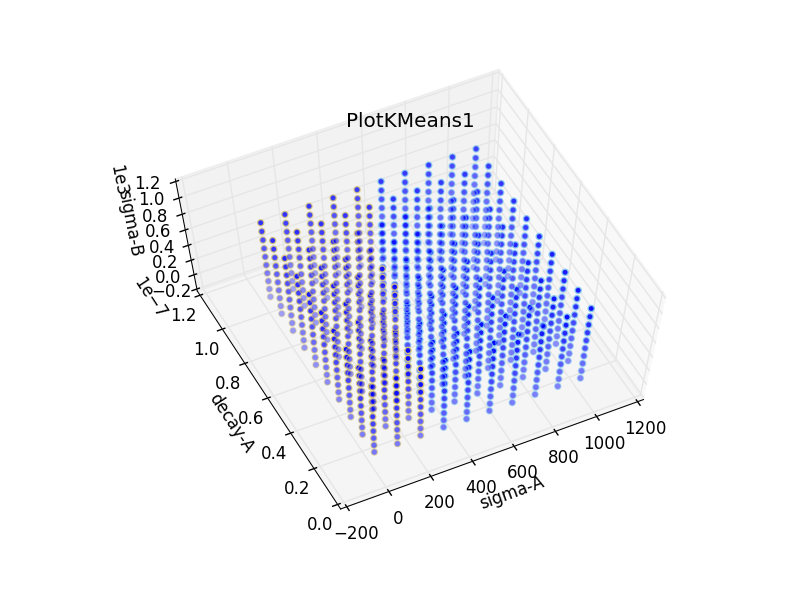
\includegraphics[scale=0.7]{pics/dataminingK-means.png}
  \caption{K-means clustering on original dataset.}
  \label{fig:KmeanOrigData}
 \end{figure}
   \item \textbf{\textit{Steps}}:   
\begin{lstlisting}[style=XML,morekeywords={arg,extension,pauseAtEnd,overwrite}]
  <Steps>
    <MultiRun name="sampleMC">
      <Input   class="Files"       type="input">referenceInput.xml</Input>
      <Model   class="Models"      type="Code">testModel</Model>
      <Sampler class="Samplers"    type="Grid">grid</Sampler>
      <Output  class="DataObjects" type="PointSet">samplesMC</Output>
      <Output  class="DataObjects" type="HistorySet">histories</Output>
    </MultiRun>
    <PostProcess name="kmeans" pauseAtEnd="True">
      <Input class="DataObjects" type="PointSet">samplesMC</Input>
      <Model class="Models" type="PostProcessor">KMeans1</Model>
      <Output class="DataObjects" type="PointSet">samplesMC</Output>
      <Output class="OutStreamManager" type="Plot">PlotKMeans1</Output>
      <Output class="OutStreamManager" type="Plot">PlotAll</Output>
      <Output class="OutStreamManager" type="Print">samplesMCdump</Output>
    </PostProcess>
    <PostProcess name="pca" pauseAtEnd="True">
      <Input class="DataObjects" type="PointSet">samplesMC</Input>
      <Model class="Models" type="PostProcessor">PCA1</Model>
      <Output class="DataObjects" type="PointSet">samplesMC</Output>
      <Output class="OutStreamManager" type="Plot">PlotPCA1</Output>
    </PostProcess>
  </Steps>
\end{lstlisting}

 %%%%%%%%%%%%%%%%%%%%%%%%%%%%%%%%%%%%%%%%%%%%%%%%%%%%%%%%%%
 %%%%%%%%%%%%%%%%%%%%%%%%%%%%%%%%%%%%%%%%%%%%%%%%%%%%%%%%%%
   Finally, all the previously defined \textbf{Entities} can be combined in 
   the \xmlNode{Steps} block; 
   3 \xmlNode{Steps} have been inputted:
   \begin{itemize}
     \item \xmlNode{MultiRun} named ``sampleMC'', used to run the 
     multiple  
     instances of the driven code and 
     collect the outputs in the two \textit{DataObjects}.The \xmlNode{Sampler} is inputted to communicate to the 
     \textit{Step} that the driven code needs to
     be perturbed through the Grid sampling strategy;
     \item \xmlNode{PostProcess} named ``kmeans'', used
     to analyze the data obtained through the sampling strategy. In
     this step, a K-Means algorithm is going to be employed, plotting
     the clustering results;
     \textit{Step} that the driven code needs to
     be perturbed through the Grid sampling strategy;
     \item \xmlNode{PostProcess} named ``pca'', used
     to analyze the data obtained through the sampling strategy. In
     this Step, a PCA algorithm is going to be employed, plotting
     the decomposition results.
   \end{itemize}
\end{enumerate} 
Figure~\ref{fig:KmeanOrigData} shows the clustering on the original
input space. 
\\Figure~\ref{fig:KmeanProjected} shows the clustering on the projected
input space. It can be noticed, that the algorithm fully capture the fact
that the parameter $sigma-B$ does not impact the response $A$ (being completely independent).
\\Figure~\ref{fig:PCAplot} shows the PCA decomposition on the data set.
%%%%%%%%%%%%%%%%%%%%%%%%%%%%%%%%%%%%%%%%%%%%%%%%%%%%%%%%%%
 %figure samples
 \begin{figure}[h!]
  \centering
  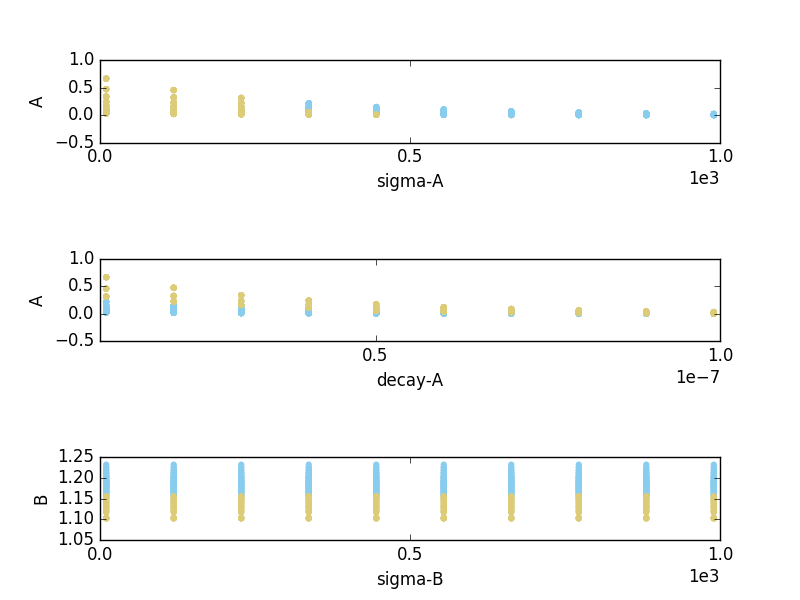
\includegraphics[scale=0.7]{pics/dataminingPlotallK-means.png}
  \caption{K-means clustering on projected parameters.}
  \label{fig:KmeanProjected}
 \end{figure}
 %%%%%%%%%%%%%%%%%%%%%%%%
 %%%%%%%%%%%%%%%%%%%%%%%%%%%%%%%%%%%%%%%%%%%%%%%%%%%%%%%%%%

 %%%%%%%%%%%%%%%%%%%%%%%%
  %%%%%%%%%%%%%%%%%%%%%%%%%%%%%%%%%%%%%%%%%%%%%%%%%%%%%%%%%%
 %figure samples
 \begin{figure}[h!]
  \centering
  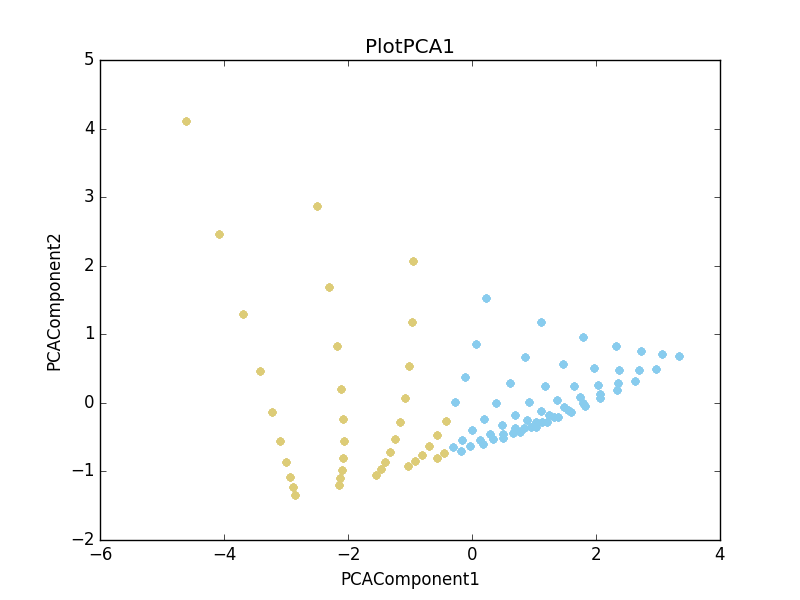
\includegraphics[scale=0.7]{pics/dataminingPCA.png}
  \caption{Principal Component Analysis.}
  \label{fig:PCAplot}
 \end{figure}
 %%%%%%%%%%%%%%%%%%%%%%%%
 
\clearpage
\begin{appendices}
 \section{Running RAVEN}

% I don't think this is mentioned earlier? Andrea answers :D It mentioned in the Introduction
%As already mentioned, 
The RAVEN code is a mixture of C++, C, and Python software. The entry point 
resides on the Python side and is accessible via a command line interface.
%
After following the instructions in the previous Section, RAVEN is ready to be
used. 
%
The RAVEN driver is contained in the folder ``\texttt{raven/framework}.''
%
To run RAVEN, open a terminal and use the following command (replace \texttt{<inputFileName.xml>} with your RAVEN input file):

\begin{lstlisting}[language=bash]
python raven/framework/Driver.py <inputFileName.xml>
\end{lstlisting}

\end{appendices}
%\appendix
\section{Appendix: Example Primer}
\label{sec:examplePrimer}
In this Appendix, a set of examples are reported. In order to be as general as possible, the \textit{Model} type ``ExternalModel'' has been used.
%%%% EXAMPLE 1 
\subsection{Example 1.}
\label{subsec:ex1}
This simple example is about the construction of a ``Lorentz attractor'', sampling the relative input space. The parameters that are sampled represent the initial coordinate (x0,y0,z0) of the attractor origin. 

\begin{lstlisting}[style=XML,morekeywords={debug,re,seeding,class,subType,limit}]
<?xml version="1.0" encoding="UTF-8"?>
<Simulation verbosity="debug">
<!-- RUNINFO -->
<RunInfo>
    <WorkingDir>externalModel</WorkingDir>
    <Sequence>FirstMRun</Sequence>
    <batchSize>3</batchSize>
</RunInfo>
<!-- Files -->
<Files>
    <Input name='lorentzAttractor.py' type=''>lorentzAttractor</Input>
</Files>
<!-- STEPS -->
<Steps>
    <MultiRun name='FirstMRun'  re-seeding='25061978'>
        <Input   class='Files'     type=''               >lorentzAttractor.py</Input>
        <Model   class='Models'    type='ExternalModel'  >PythonModule</Model>
        <Sampler class='Samplers'  type='MonteCarlo'     >MC_external</Sampler>
        <Output  class='DataObjects'     type='HistorySet'      >testPrintHistorySet</Output>
        <Output  class='Databases' type='HDF5'           >test_external_db</Output>
        <Output  class='OutStreamManager' type='Print'   >testPrintHistorySet_dump</Output>
    </MultiRun >
</Steps>
<!-- MODELS -->
<Models>
    <ExternalModel name='PythonModule' subType='' ModuleToLoad='externalModel/lorentzAttractor'>  
       <variable>sigma</variable>
       <variable>rho</variable>
       <variable>beta</variable>
       <variable>x</variable>
       <variable>y</variable>
       <variable>z</variable>
       <variable>time</variable>
       <variable>x0</variable>
       <variable>y0</variable>
       <variable>z0</variable>
    </ExternalModel>
</Models>
<!-- DISTRIBUTIONS -->
<Distributions>
    <Normal name='x0_distrib'>
        <mean>4</mean>
        <sigma>1</sigma>
    </Normal>
    <Normal name='y0_distrib'>
        <mean>4</mean>
        <sigma>1</sigma>
    </Normal>
    <Normal name='z0_distrib'>
        <mean>4</mean>
        <sigma>1</sigma>
    </Normal>
</Distributions>
<!-- SAMPLERS -->
<Samplers>
    <MonteCarlo name='MC_external'>
      <sampler_init>
        <limit>3</limit>
      </sampler_init>
      <variable name='x0' >
        <distribution  >x0_distrib</distribution>
      </variable>
      <variable name='y0' >
        <distribution  >y0_distrib</distribution>
      </variable>
      <variable name='z0' >
        <distribution  >z0_distrib</distribution>
      </variable>
    </MonteCarlo>
</Samplers>
<!-- DATABASES -->
<Databases>
  <HDF5 name="test_external_db"/>
</Databases>
<!-- OUTSTREAMS -->
<OutStreamManager>
  <Print name='testPrintHistorySet_dump'>
    <type>csv</type>
    <source>testPrintHistorySet</source>
  </Print>
</OutStreamManager>
<!-- DATA OBJECTS -->
<DataObjects>
    <HistorySet name='testPrintHistorySet'>
        <Input>x0,y0,z0</Input>
        <Output>time,x,y,z</Output>
   </HistorySet>
</DataObjects>
</Simulation>
\end{lstlisting}
The Python \textit{ExternalModel} is reported below:
\begin{lstlisting}[language=python]
import numpy as np

def run(self,Input):
  max_time = 0.03
  t_step = 0.01

  numberTimeSteps = int(max_time/t_step)

  self.x = np.zeros(numberTimeSteps)
  self.y = np.zeros(numberTimeSteps)
  self.z = np.zeros(numberTimeSteps)
  self.time = np.zeros(numberTimeSteps)

  self.x0 = Input['x0']
  self.y0 = Input['y0']
  self.z0 = Input['z0']

  self.x[0] = Input['x0']
  self.y[0] = Input['y0']
  self.z[0] = Input['z0']
  self.time[0]= 0

  for t in range (numberTimeSteps-1):
    self.time[t+1] = self.time[t] + t_step
    self.x[t+1]    = self.x[t] +  self.sigma*
                      (self.y[t]-self.x[t]) * t_step
    self.y[t+1]    = self.y[t] + (self.x[t]*
                      (self.rho-self.z[t])-self.y[t]) * t_step
    self.z[t+1]    = self.z[t] + (self.x[t]*
                          self.y[t]-self.beta*self.z[t]) * t_step
\end{lstlisting}
%%%% EXAMPLE 2 
\subsection{Example 2.}
\label{subsec:ex1}
This example shows a slightly more complicated example, that employs the usage of:
\begin{itemize}
    \item \textit{Samplers:} Grid and Adaptive;
    \item \textit{Models:} External, Reduce Order Models and Post-Processors;
    \item \textit{OutStreams:} Prints and Plots;
    \item \textit{Data Objects:} PointSets;
    \item \textit{Functions:} ExternalFunctions.
\end{itemize}
The goal of this input is to compute the ``SafestPoint''.
It provides the coordinates of the farthest
point from the limit surface that is given as an input.
%
The safest point coordinates are expected values of the coordinates of the
farthest points from the limit surface in the space of the ``controllable''
variables based on the probability distributions of the ``non-controllable''
variables.

The term ``controllable'' identifies those variables that are under control
during the system operation, while the ``non-controllable'' variables are
stochastic parameters affecting the system behaviour randomly.

The ``SafestPoint'' post-processor requires the set of points belonging to the
limit surface, which must be given as an input.

\begin{lstlisting}[style=XML,morekeywords={debug,re,seeding,class,subType,limit}]
<Simulation verbosity='debug'>

<!-- RUNINFO -->
<RunInfo>
  <WorkingDir>SafestPointPP</WorkingDir>
  <Sequence>pth1,pth2,pth3,pth4</Sequence>
  <batchSize>50</batchSize>
</RunInfo>

<!-- STEPS -->
<Steps>  
  <MultiRun name = 'pth1' pauseAtEnd = 'False'>
    <Sampler  class = 'Samplers'  type = 'Grid'           >grd_vl_ql_smp_dpt</Sampler>
    <Input    class = 'DataObjects'     type = 'PointSet'   >grd_vl_ql_smp_dpt_dt</Input>
    <Model    class = 'Models'    type = 'ExternalModel'  >xtr_mdl</Model>
    <Output   class = 'DataObjects'     type = 'PointSet'   >nt_phy_dpt_dt</Output>    
  </MultiRun >
  
  <MultiRun name = 'pth2' pauseAtEnd = 'True'>
    <Sampler          class = 'Samplers'  type = 'Adaptive'      >dpt_smp</Sampler>
    <Input            class = 'DataObjects'     type = 'PointSet'  >bln_smp_dt</Input>   
    <Model            class = 'Models'    type = 'ExternalModel' >xtr_mdl</Model>
    <Output           class = 'DataObjects'     type = 'PointSet'  >nt_phy_dpt_dt</Output>            
    <SolutionExport   class = 'DataObjects'     type = 'PointSet'  >lmt_srf_dt</SolutionExport>
  </MultiRun>
  
  <PostProcess name='pth3' pauseAtEnd = 'False'>
    <Input    class = 'DataObjects'          type = 'PointSet'       >lmt_srf_dt</Input>
    <Model    class = 'Models'         type = 'PostProcessor'  >SP</Model>
    <Output   class = 'DataObjects'          type = 'PointSet'     >sfs_pnt_dt</Output>
  </PostProcess>  
  
  <OutStreamStep name = 'pth4' pauseAtEnd = 'True'>
  	<Input  class = 'DataObjects'            type = 'PointSet'  >lmt_srf_dt</Input>
  	<Output class = 'OutStreamManager' type = 'Print'         >lmt_srf_dmp</Output>
    <Input  class = 'DataObjects'            type = 'PointSet'  >sfs_pnt_dt</Input>
  	<Output class = 'OutStreamManager' type = 'Print'         >sfs_pnt_dmp</Output>
  </OutStreamStep>
</Steps>

<!-- DATA OBJECTS -->
<DataObjects> 
  <PointSet name = 'grd_vl_ql_smp_dpt_dt'>
    <Input>x1,x2,gammay</Input>
    <Output>OutputPlaceHolder</Output>
  </PointSet>
  
  <PointSet name = 'nt_phy_dpt_dt'>
    <Input>x1,x2,gammay</Input>
    <Output>g</Output>
  </PointSet>
    
  <PointSet name = 'bln_smp_dt'>
    <Input>x1,x2,gammay</Input>
    <Output>OutputPlaceHolder</Output>
  </PointSet>
    
  <PointSet name = 'lmt_srf_dt'>
    <Input>x1,x2,gammay</Input>
    <Output>g_zr</Output>
  </PointSet>
  
  <PointSet name = 'sfs_pnt_dt'>
    <Input>x1,x2,gammay</Input>
    <Output>p</Output>
  </PointSet>
</DataObjects>

<!-- DISTRIBUTIONS -->
<Distributions>
  <Normal name = 'x1_dst'>
    <upperBound>10</upperBound>
    <lowerBound>-10</lowerBound>
  	<mean>0.5</mean>
    <sigma>0.1</sigma>
  </Normal>
  
  <Normal name = 'x2_dst'>
    <upperBound>10</upperBound>
    <lowerBound>-10</lowerBound>
    <mean>-0.15</mean>
    <sigma>0.05</sigma>
  </Normal>
  
  <Normal name = 'gammay_dst'>
    <upperBound>20</upperBound>
    <lowerBound>-20</lowerBound>
    <mean>0</mean>
    <sigma>15</sigma>
  </Normal>
</Distributions>

<!-- SAMPLERS -->
<Samplers>  
  <Grid name = 'grd_vl_ql_smp_dpt'>
    <variable name = 'x1' >
      <distribution>x1_dst</distribution>
      <grid type = 'value' construction = 'equal' steps = '10' upperBound = '10'>2</grid>
    </variable>  
    <variable name='x2' >
      <distribution>x2_dst</distribution>
      <grid type = 'value' construction = 'equal' steps = '10' upperBound = '10'>2</grid>
    </variable>
    <variable name='gammay' >
      <distribution>gammay_dst</distribution>
      <grid type = 'value' construction = 'equal' steps = '10' lowerBound = '-20'>4</grid>
    </variable>
  </Grid>
  
  <Adaptive name = 'dpt_smp' verbosity='debug'>
    <ROM              class = 'Models'    type = 'ROM'           >accelerated_ROM</ROM>
    <Function         class = 'Functions' type = 'External'      >g_zr</Function>
    <TargetEvaluation class = 'DataObjects'     type = 'PointSet'  >nt_phy_dpt_dt</TargetEvaluation>
    <Convergence limit = '3000' forceIteration = 'False' weight = 'none' persistence = '5'>1e-2</Convergence>
      <variable name = 'x1'>
        <distribution>x1_dst</distribution>
      </variable>
      <variable name = 'x2'>
        <distribution>x2_dst</distribution>
      </variable>
      <variable name = 'gammay'>
        <distribution>gammay_dst</distribution>
      </variable>
  </Adaptive>
</Samplers>

<!-- MODELS -->
<Models>  
  <ExternalModel name = 'xtr_mdl' subType = '' ModuleToLoad = 'SafestPointPP/safest_point_test_xtr_mdl'>
    <variable>x1</variable>
    <variable>x2</variable>
    <variable>gammay</variable>
    <variable>g</variable>
  </ExternalModel>
  
  <ROM name = 'accelerated_ROM' subType = 'SciKitLearn'>
    <Features>x1,x2,gammay</Features>
    <Target>g_zr</Target>
    <SKLtype>svm|SVC</SKLtype>
    <kernel>rbf</kernel>
    <gamma>10</gamma>
    <tol>1e-5</tol>
    <C>50</C>
  </ROM>

  <PostProcessor name='SP' subType='SafestPoint'>
    <!-- List of Objects (external with respect to this PP) needed by this post-processor -->
    <Distribution     class = 'Distributions'  type = 'Normal'>x1_dst</Distribution>
    <Distribution     class = 'Distributions'  type = 'Normal'>x2_dst</Distribution>
    <Distribution     class = 'Distributions'  type = 'Normal'>gammay_dst</Distribution>
    <!- end of the list -->
    <controllable>
    	<variable name = 'x1'>
    		<distribution>x1_dst</distribution>
    		<grid type = 'value' steps = '20'>1</grid>   		
    	</variable>
    	<variable name = 'x2'>
    		<distribution>x2_dst</distribution>
    		<grid type = 'value' steps = '20'>1</grid>   		
    	</variable>
    </controllable>
    <non-controllable>
    	<variable name = 'gammay'>
    		<distribution>gammay_dst</distribution>
    		<grid type = 'value' steps = '20'>2</grid>
    	</variable> 	
    </non-controllable>
  </PostProcessor>
</Models>

<!-- FUNCTIONS -->
<Functions>
  <External name='g_zr' file='SafestPointPP/safest_point_test_g_zr.py'>
    <variable>g</variable>
  </External>
</Functions>

<!-- OUT-STREAMS -->
<OutStreamManager> 
  <Print name = 'lmt_srf_dmp'>
  	<type>csv</type>
  	<source>lmt_srf_dt</source>
  </Print>
  
  <Print name = 'sfs_pnt_dmp'>
  	<type>csv</type>
  	<source>sfs_pnt_dt</source>
  </Print>
</OutStreamManager>

</Simulation>
\end{lstlisting}
The Python \textit{ExternalModel} is reported below:
\begin{lstlisting}[language=python]
def run(self,Input): 
  self.g = self.x1+4*self.x2-self.gammay
\end{lstlisting}
The ``Goal Function'',the function that defines the transitions with respect the input space coordinates, is as follows:
\begin{lstlisting}[language=python]
def __residuumSign(self):
  if self.g<0 : return  1
  else        : return -1
\end{lstlisting}

%%%%% EXAMPLE 3
%\subsection{Example3}
%\label{subsec:ex1}
%example 3



    % ---------------------------------------------------------------------- %
    % References
    %
    \clearpage
    % If hyperref is included, then \phantomsection is already defined.
    % If not, we need to define it.
    \providecommand*{\phantomsection}{}
    \phantomsection
    \addcontentsline{toc}{section}{References}
    \bibliographystyle{ieeetr}
    \bibliography{raven_user_guide}


    % ---------------------------------------------------------------------- %
    %

    % \printindex

    %\include{distribution}

\end{document}
